\chapter{Complex Networks Experiments}
\label{chap:Four}

\section{Introduction}
In this chapter, experiments with more complex networks have been performed.
An introduction to these networks and the reasons behind their selection has been
covered in the begging of the chapter. The experiments structure, for each topology,
have also been analyzed and illustrated with pseudo code. Finally, an analysis on
the data produced for these experiments, has been performed.

The issues raised in~\ref{chap:Three}, have been address in the current chapter,
altering various approaches. For example, a measure of similarity between the
strategies has been used. The measure used, is based on the average cooperating
ratio of the strategies. Furthermore, median ranking of each strategy has been
looked into, for it is believed to be a more appropriate measure of performance,
compared to winning ratio. Regression models for the median rank have been build
and Kruskal Wallis analysis has been held. Furthermore, round robin in treated as
a spatial tournament of a complete topology.

\subsection{Networks}

A complex network is a graph with non-trivial topological features;
features that can not occur in networks such as the ones studied in ~\ref{chap:Three}.
Such features include, a heavy tail in the degree distribution, a high
clustering coefficient, and hierarchical structure. Complex networks are commonly
used to study computer network, technological networks and social networks.

They will also be used in the experiment conducted in this dissertation. Small
world and random graphs, and more specifically, the following networks are
studied :

\begin{itemize}
	\item Watts-Strogatz, a model for generating graphs with small-world properties
	\item Erdős–Rényi, a model for generating random graphs
	\item Complete Graph, a graph with the properties of a round robin topology
\end{itemize}

Each of the experiment has a different set of parameters, thus the size of
data produced by each experiment is different. The structure of each experiment
is analyzed on the following subsection.

\subsection{Experiments Structure}
\label{sub:experiments-structure}
\subsubsection{Small-world}

Watts Strogatz, is the small world graph generator model used in this experiment.
The Watts Strogatz model, was proposed by D. Watss and S. Strogatz,
(whose name was used), in their work in 1998~\cite{Watts1998}.
Their works was aimed to reproduce a network/graph, which was somewhere between
a regular and a random network. To interpolate between regular and random
networks, they considered a random rewiring procedure. Starting from a ring
lattice with \(n\) vertices and \(k\) edges per vertex, each edge is being
rewired, at random, with a probability of \(p\).

Networkx, provides a function for the given model. The documentation for the
Watts Strogatz function, can be found here
\url{https://networkx.github.io/documentation/development/reference/generated/networkx.generators.random_graphs.watts_strogatz_graph.html#networkx.generators.random_graphs.watts_strogatz_graph}
, and the given arguments are \(n\), \(k\) and \(p\). Moreover,
the tournament size is not going to be deterministic, it will
range from 2 to 50. Similarly for the initial size, it will range from 2
to tournament size minus one. The chosen players are also shuffled and re placed
on the graph. A pseudo code illustrating the structure of the experiment is shown
in~\ref{small-world-experiment}:


\begin{algorithm}
	\caption{Small world Experiment}\label{small-world-experiment}
	\begin{algorithmic}
		\Procedure{Small World}{}
		\BState \emph{loop}:
		\For {$\textit{tournament.size} \gets \textit{ 2 to 50}$}
		\For {$\textit{initial.neighborhood.size} \gets \textit{1 to tournament.size-1}$}
		\For {$\textit{i} \gets \textit{ 0 to 10}$}
		\State $player \gets \textit{random.strategies}$.
		\For {$p \gets \textit{0 to 10}$}
		\State $G \gets \textit{create.watts.strogatz.graph}$.
		\State $edges \gets \textit{G.egdes}$
		\State $results \gets \textit{play.tournament}$.
		\emph{loop}.
		\EndFor
		\EndFor
		\EndFor
		\EndFor
		\EndProcedure
	\end{algorithmic}
\end{algorithm}

\subsubsection{Random}

For recreating a random network experiment, Erd\"{o}s–R\'{e}nyi model was used.
The model is named after P. Erd\"{o}s and A. R\'{e}nyi, who introduced
the model in 1959~\cite{Erdos1959}. It generates a random graph of \(n\)
vertices and chooses each of the possible edges with probability \(p\).

Once again, networkx provide a function to easily generate such graph
\url{https://networkx.github.io/documentation/development/reference/generated/networkx.generators.random_graphs.binomial_graph.html#networkx.generators.random_graphs.binomial_graph}.
The arguments taken but the function are \(n\)  and \(p\) as the probability for
edge creation. Similarly, the tournament size is not going to be deterministic.
The tournament size will range from 2 to 50. The chosen players are also shuffled
and re placed on the graph. A pseudo code illustrating the structure of the
experiment is shown in~\ref{random-experiment}:

\begin{algorithm}
	\caption{Random Experiment}\label{random-experiment}
	\begin{algorithmic}
		\Procedure{Random}{}
		\BState \emph{loop}:
		\For {$\textit{tournament.size} \gets \textit{2 to 50}$}
		\For {$\textit{i} \gets \textit{ 0 to 100}$}
		\State $player \gets \textit{random.strategies}$.
		\For {$p \gets \textit{0 to 10}$}
		\State $G \gets \textit{create.erdos.renyi.graph}$.
		\State $edges \gets \textit{G.egdes}$
		\State $results \gets \textit{play.tournament}$.
		\emph{loop}.
		\EndFor
		\EndFor
		\EndFor
		\EndProcedure
	\end{algorithmic}
\end{algorithm}

\subsubsection{Complete}

In the previous chapter, ~\ref{ch:Three}, the round robin experiment was
conducted by the \texttt{RoundRobinTournament} class, in this experiment the
\texttt{SpatialTournament} class is used.
The following networx function is used(\url{https://networkx.github.io/documentation/development/reference/generated/networkx.generators.classic.complete_graph.html#networkx.generators.classic.complete_graph}).
, to generate a complete graph. The following pseudo-code explain the structure
of the experiment ~\ref{complete-experiment}.

\begin{algorithm}
	\caption{Complex Experiments Rules}\label{complete-experiment}
	\begin{algorithmic}
		\Procedure{Complete}{}
		\BState \emph{loop}:
		\For {$\textit{tournament.size} \gets \textit{2 to 50}$}
		\For {$\textit{i} \gets \textit{ 0 to 100}$}
		\State $player \gets \textit{random.strategies}$.
		\State $G \gets \textit{create.complete.graph}$.
		\State $edges \gets \textit{G.egdes}$
		\State $results \gets \textit{play.tournament}$.
		\emph{loop}.
		\EndFor
		\EndFor
		\EndProcedure
	\end{algorithmic}
\end{algorithm}

\section{Preliminary Analysis}
In this section the analysis for the complex networks experiments is described.
Starting with an analysis on the networks for all three topologies, following
a preliminary analysis on the results of the experiments. The next subsection is
focused on the classification of the strategies based on the cooperation rate.

\subsection{Network Analysis}
\label{sub:network-analysis}
The networks of each experiment are studied. As introduced in ~\ref{chap:Two}, the
connectivity and clustering concepts are summarized and reviewed. Due to the
size of experiments and the time in hands, not all experiments managed to
maximize their tournament sizes, as they have been described in~\ref{sub:experiments-structure}.

More specifically, for the small world experiment, a total of 59051 graphs have
been created. The maximum number of nodes achieved is 13. Moreover, the
median degree, has been 4.75. Thus indicating that
in most tournaments, the average number of neighbors per strategy was 4.
The maximum median degree is equal to 12. Further, the mean connectivity of the
Watts Strogatz network is 3.40. Minimum value is 0 and maximum 9. Lastly,
clustering coefficient ranges from 0 to 1, with a mean of 0.48.

\begin{table}[!hbtp]
	\centering
	\begin{adjustbox}{width=0.6\textwidth}
		\small
		\begin{tabular}{|l|l|l|l|l|}
			\hline
			\multicolumn{5}{|c|}{Small world Networks Summary Table}                  \\ \hline
			     & connectivity & clustering & degree & nodes                  \\ \hline
			mean & 3.40         & 0.48       & 4.75   & 10.00                  \\ \hline
			std  & 2.37         & 0.33       & 2.65   & \multicolumn{1}{c|}{-} \\ \hline
			min  & 0.00         & 0.00       & 1.00   & 3.00                   \\ \hline
			max  & 9.00         & 1.00       & 12.00  & 13.00                  \\ \hline
		\end{tabular}
	\end{adjustbox}
	\caption{Small world Summary Table}
	\label{small-world-summary-table}
\end{table}

Illustrating 59051 graphs for understanding the networks of the experiment, is
an impossible task. For this reason, the summary table~\ref{small-world-summary-table}
has been used. A mean of 0.48, for the clustering coefficients, indicates
that strategies have a neutral trend towards creating cliques (complete graphs).
Eight networks have been randomly selected and
displayer here~\ref{small_networks_illustration}. Mainly to get an ideal of the
look of the networks in this experiment.

\begin{figure}[htp!]
	\centering
	\begin{subfigure}[t]{0.30\textwidth}
		\centering
		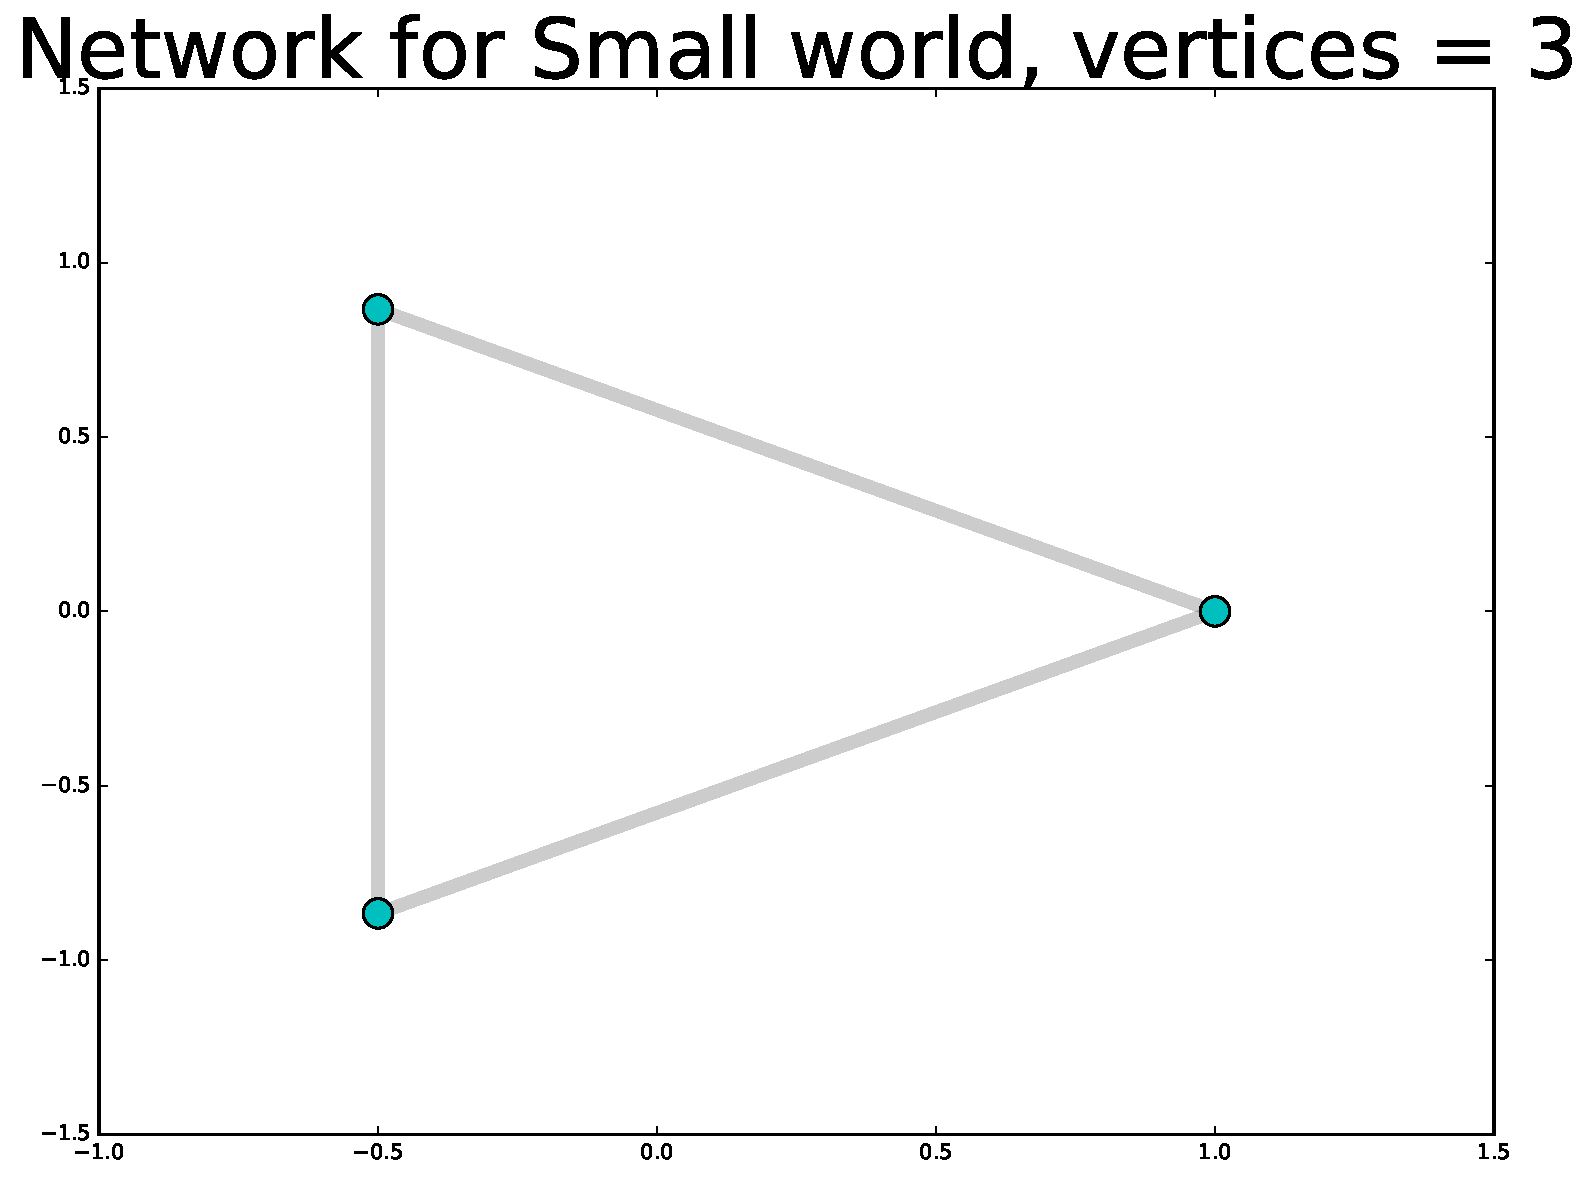
\includegraphics[width=\linewidth]{chapter-four/small__networks_3.pdf}
		\caption{Three nodes.}
	\end{subfigure}
	\hfill
	\begin{subfigure}[t]{0.30\textwidth}\centering
		\centering
		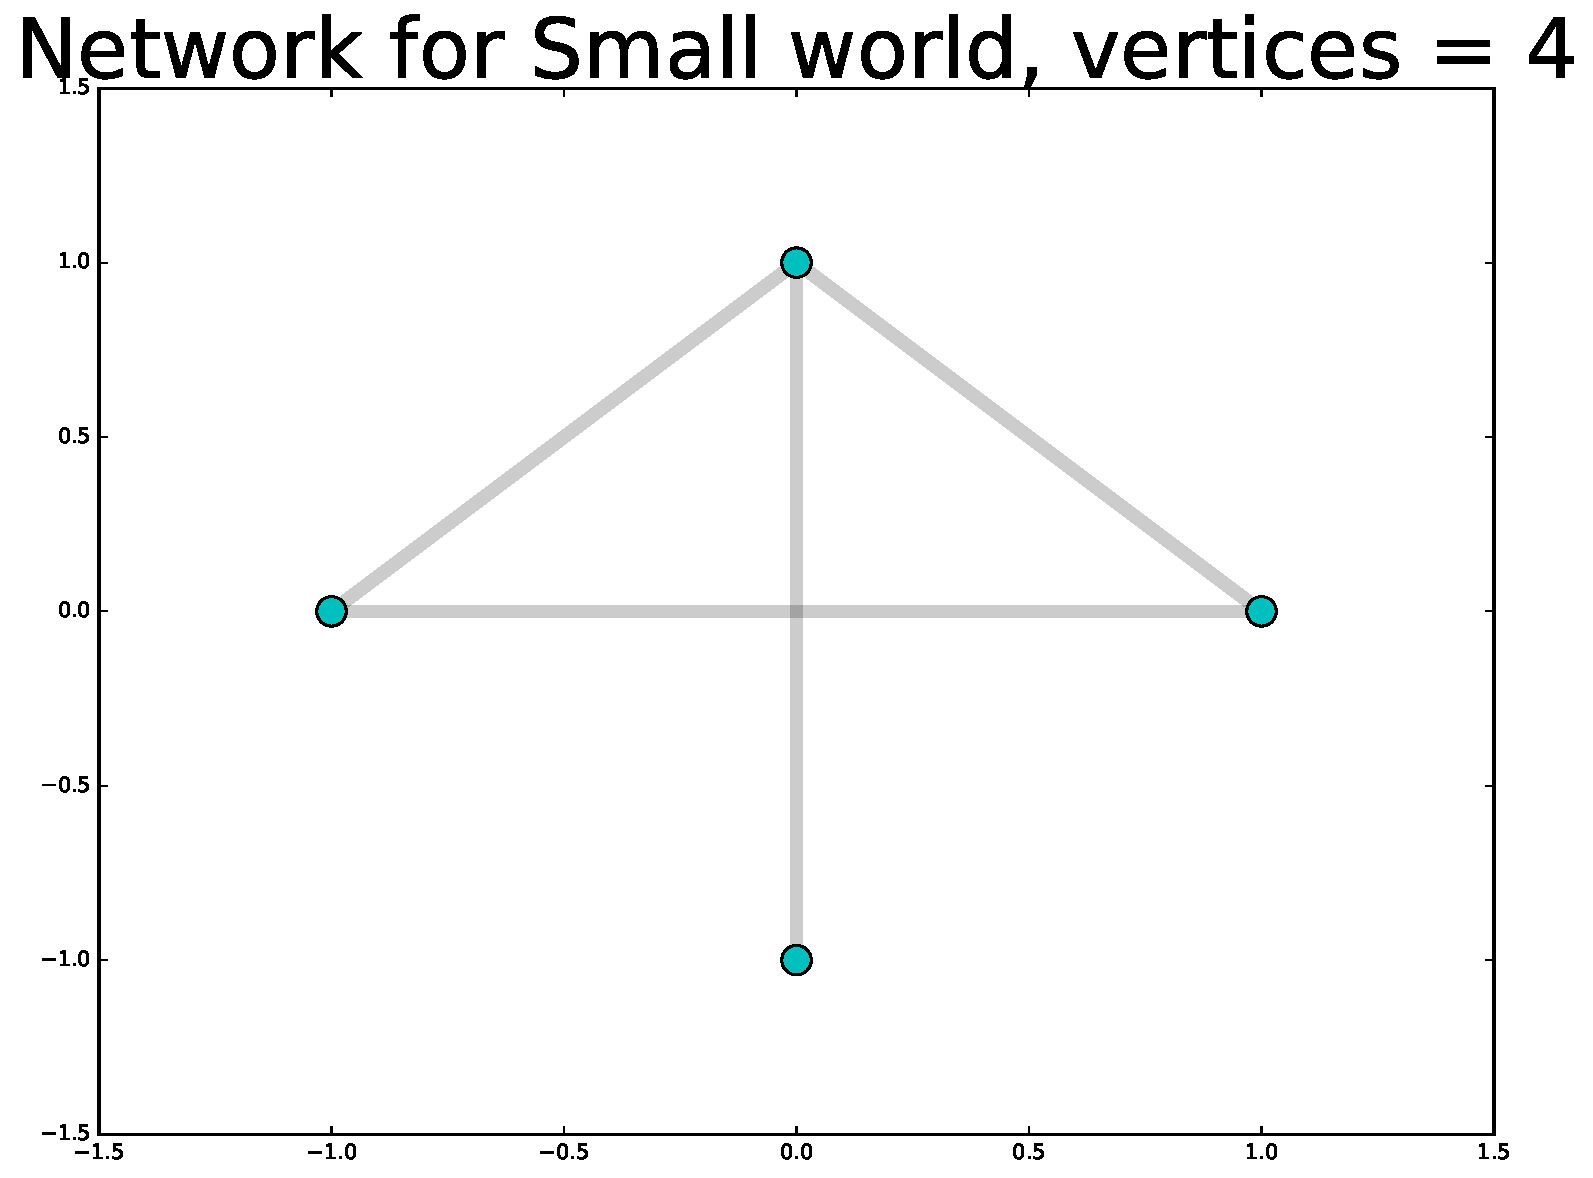
\includegraphics[width=\linewidth]{chapter-four/small__networks_4.pdf}
		\caption{Four nodes.}
	\end{subfigure}
	\hfill
	\begin{subfigure}[t]{0.30\textwidth}\centering
		\centering
		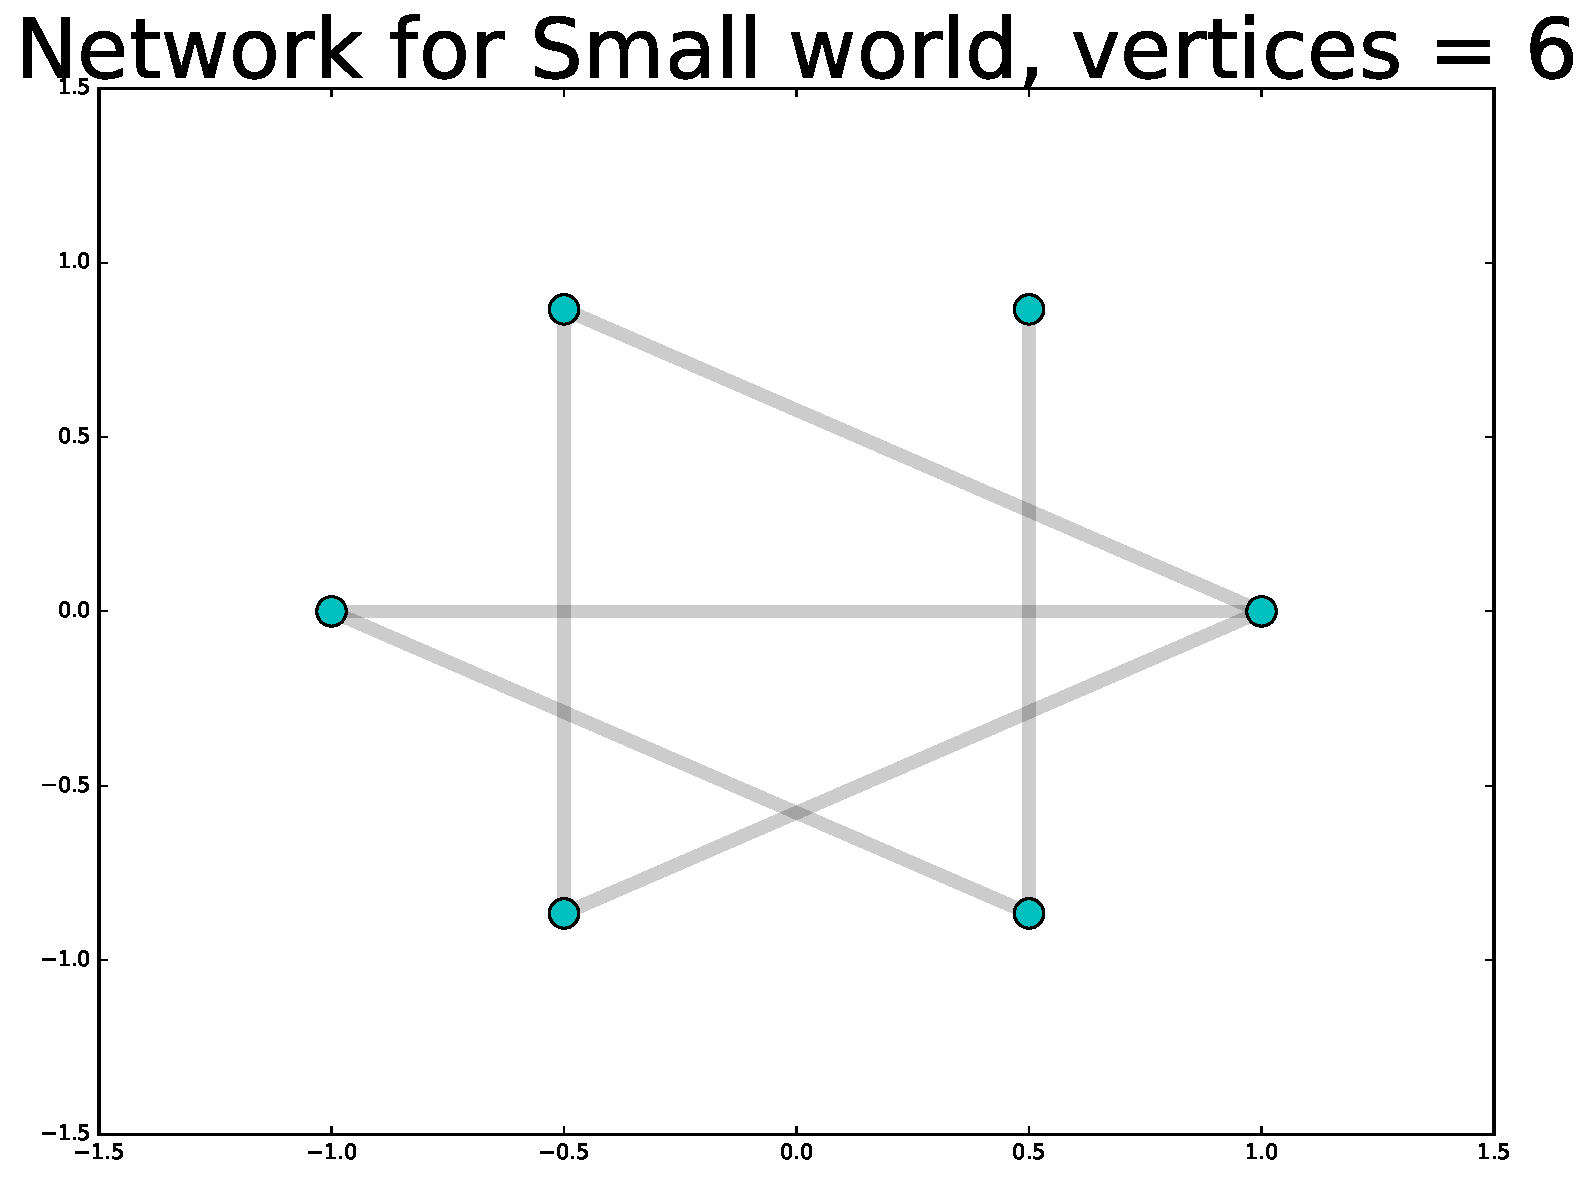
\includegraphics[width=\linewidth]{chapter-four/small__networks_6.pdf}
		\caption{Six nodes.}
	\end{subfigure}
	\hfill
	\begin{subfigure}[t]{0.30\textwidth}\centering
		\centering
		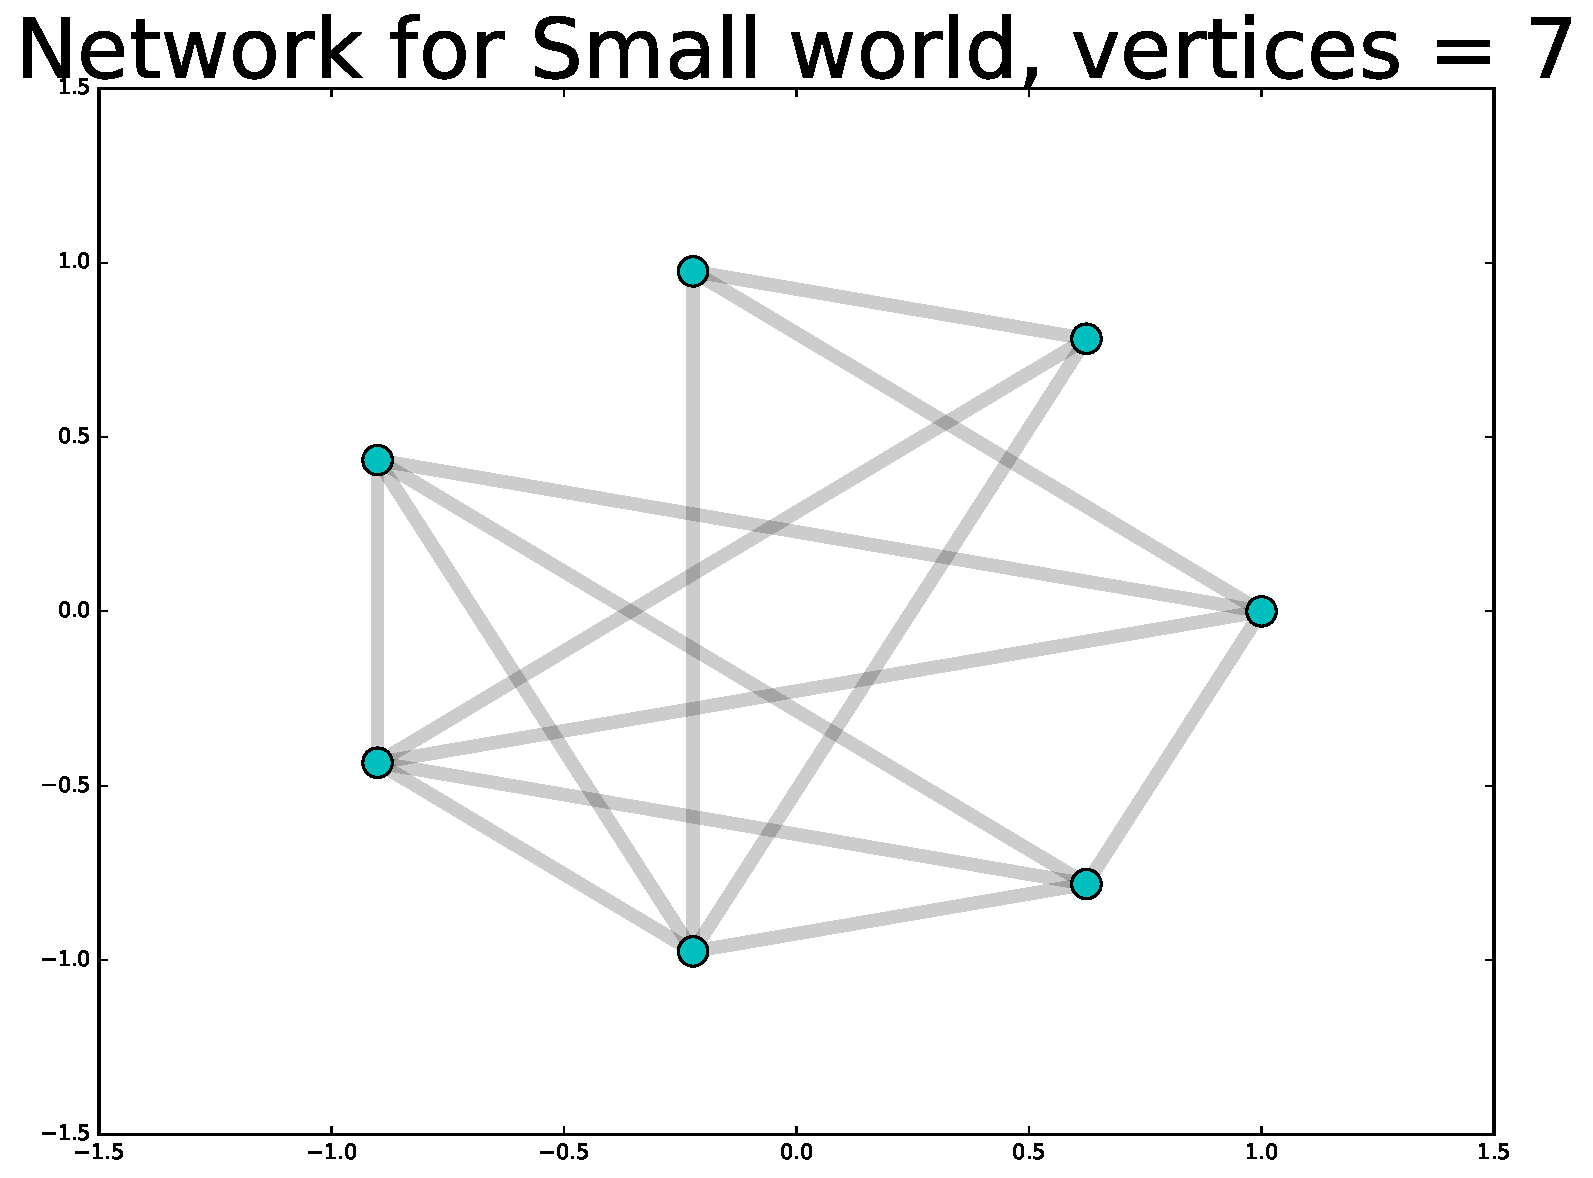
\includegraphics[width=\linewidth]{chapter-four/small__networks_7.pdf}
		\caption{Seven nodes.}
	\end{subfigure}
	\hfill
	\begin{subfigure}[t]{0.30\textwidth}\centering
		\centering
		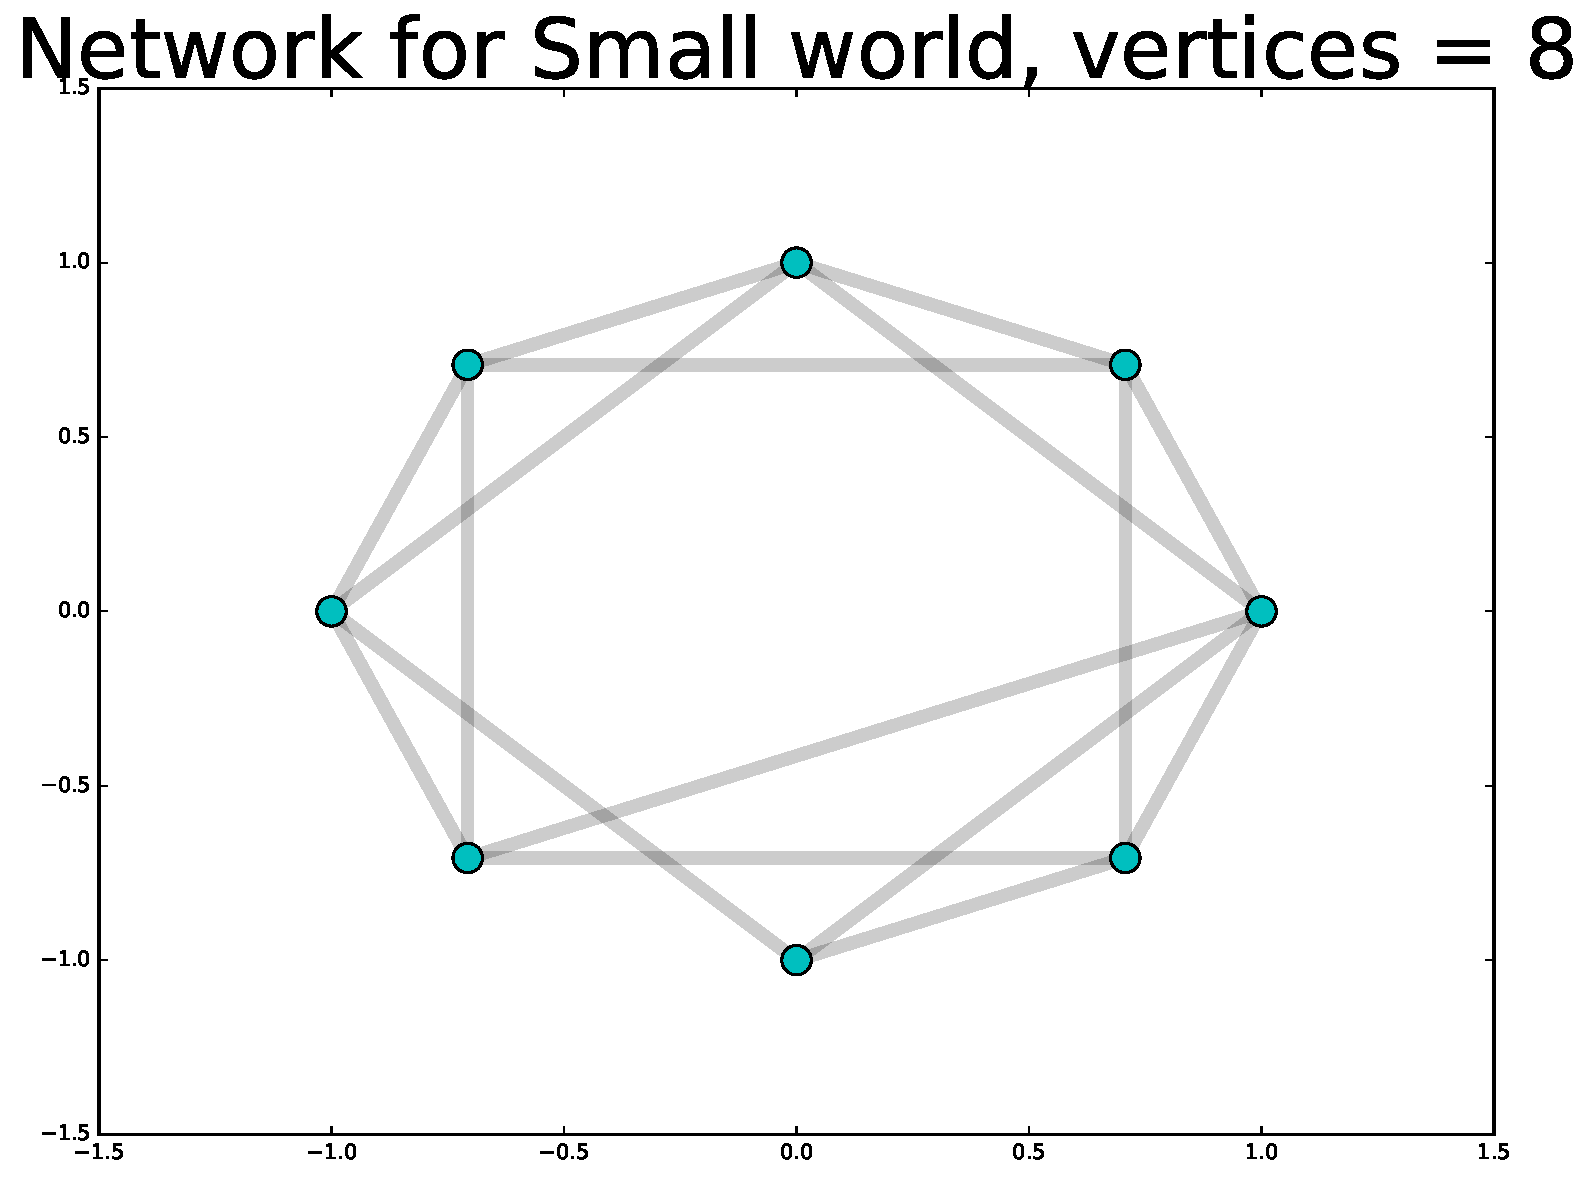
\includegraphics[width=\linewidth]{chapter-four/small__networks_8.pdf}
		\caption{Eight nodes.}
	\end{subfigure}
	\hfill
	\begin{subfigure}[t]{0.30\textwidth}\centering
		\centering
		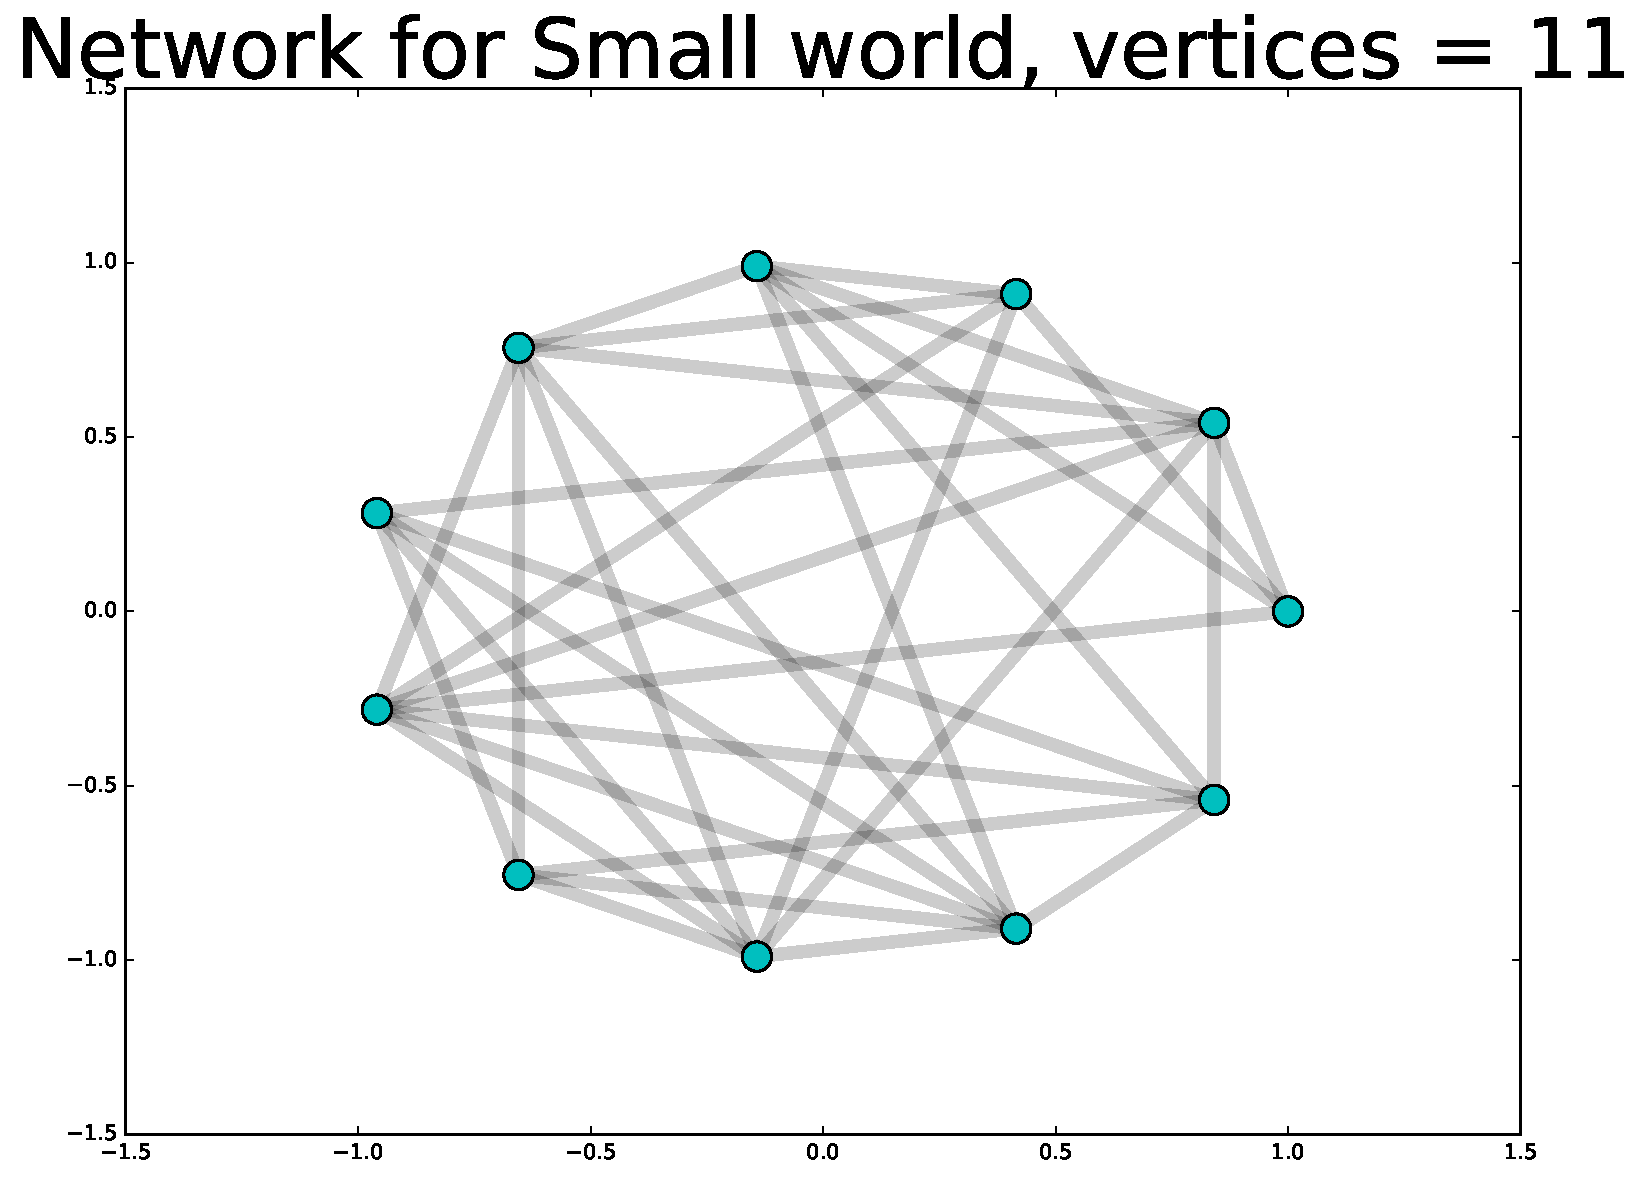
\includegraphics[width=\linewidth]{chapter-four/small__networks_11.pdf}
		\caption{Eleven nodes.}
	\end{subfigure}
	\caption{Various Watss Strogatz networks.}
	\label{small_networks_illustration}
\end{figure}

Likewise for the Erd\"{o}s R\'{e}nyi network. The experiment did not manage to
achieve the maximum tournament size that had been set. Instead, 21924 have been
created and the maximum nodes number is equal to 29. As shown in table~\ref{binomial-summary-table},
the mean number of nodes of the experiments has been 20 and the minimum 2. The
minimum number of nodes differs to these of the small world experiment, where
tournaments of two have not been able to be played. Probably, because a node
was disconnected. Binomial seems to have handled that. This can been shown
also by the connectivity, where the mean connectivity, of a random network, is
approximately 8.26. Compared to the small world that has been fairly lower,
approximately 3.

\begin{table}[!hbtp]
	\centering
	\begin{adjustbox}{width=0.6\textwidth}
		\small
		\begin{tabular}{|l|l|l|l|l|}
			\hline
			\multicolumn{5}{|c|}{Random Networks Summary Table}                       \\ \hline
			     & connectivity & clustering & degree & nodes                  \\ \hline
			mean & 8.26         & 0.60       & 11.22  & 19.80                  \\ \hline
			std  & 6.46         & 0.30       & 6.50   & \multicolumn{1}{c|}{-} \\ \hline
			min  & 0.00         & 0.00       & 1.00   & 2.00                   \\ \hline
			max  & 28.00        & 1.00       & 28.00  & 29.00                  \\ \hline
		\end{tabular}
	\end{adjustbox}
	\caption{Random Summary Table}
	\label{binomial-summary-table}
\end{table}

Another differs between the two network experiments, have occurred in the
clustering coefficient. The clustering coefficient, of the random networks has a
mean value of 0.60. Thus, the strategies tend to form groups, more in this
experiment. The mean node number is equal to 20 with a mean degree 11. Thus, in
most of the tournaments that occurred, the strategy had to compete with 11 of it's
neighbors. Once again, six random have been picked and are illustrated
in ~\ref{random_networks_illustration}.

\begin{figure}[H]
	\centering
	\begin{subfigure}[t]{0.30\textwidth}
		\centering
		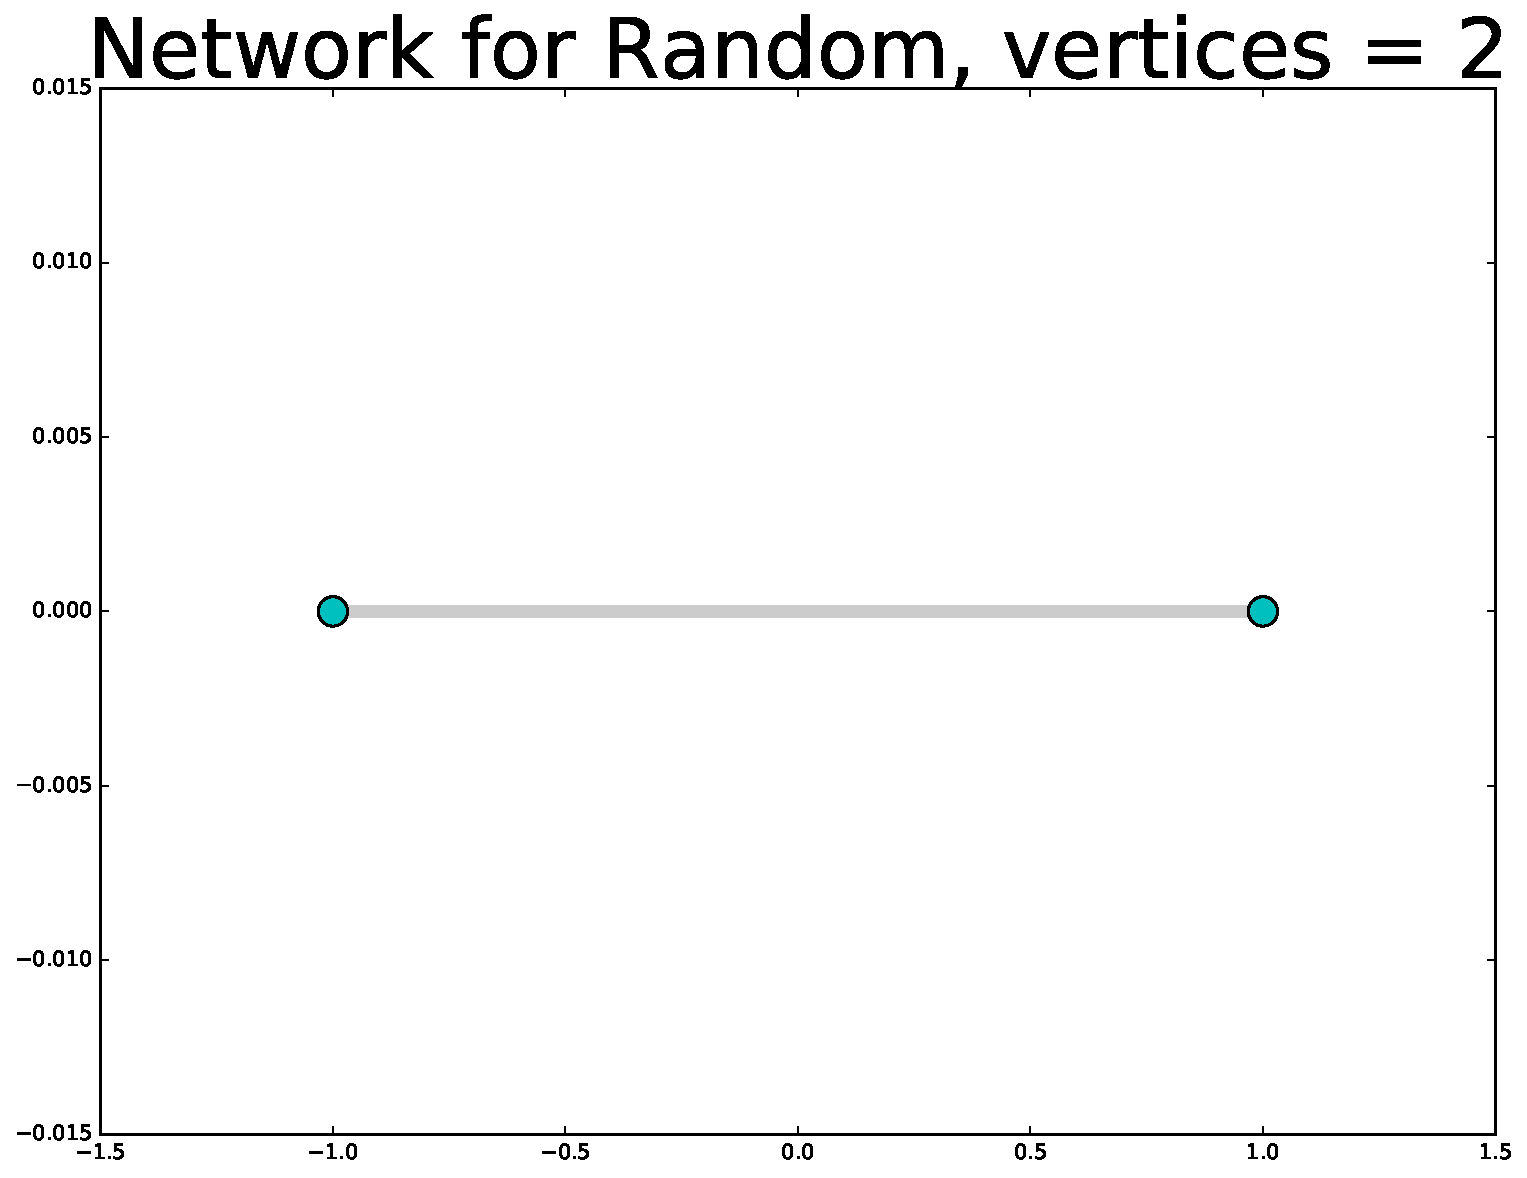
\includegraphics[width=\linewidth]{chapter-four/random_2.pdf}
		\caption{Two nodes.}
	\end{subfigure}
	\hfill
	\begin{subfigure}[t]{0.30\textwidth}\centering
		\centering
		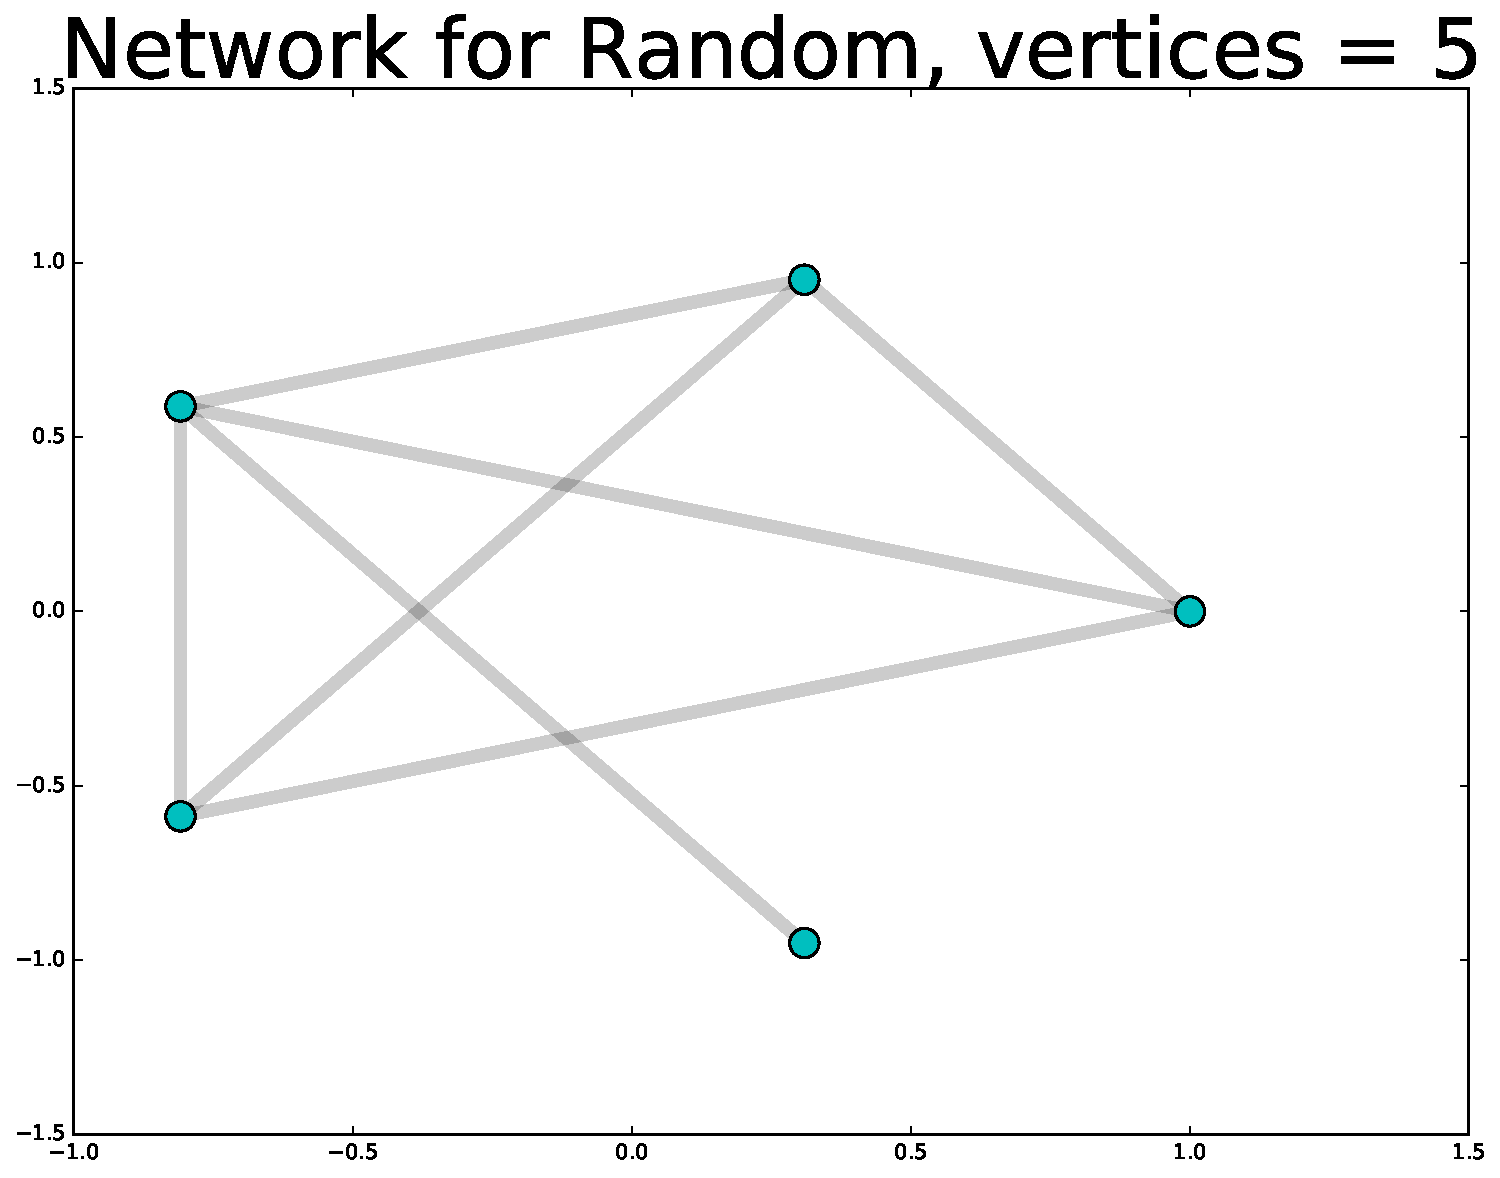
\includegraphics[width=\linewidth]{chapter-four/random_5.pdf}
		\caption{Five nodes.}
	\end{subfigure}
	\hfill
	\begin{subfigure}[t]{0.30\textwidth}\centering
		\centering
		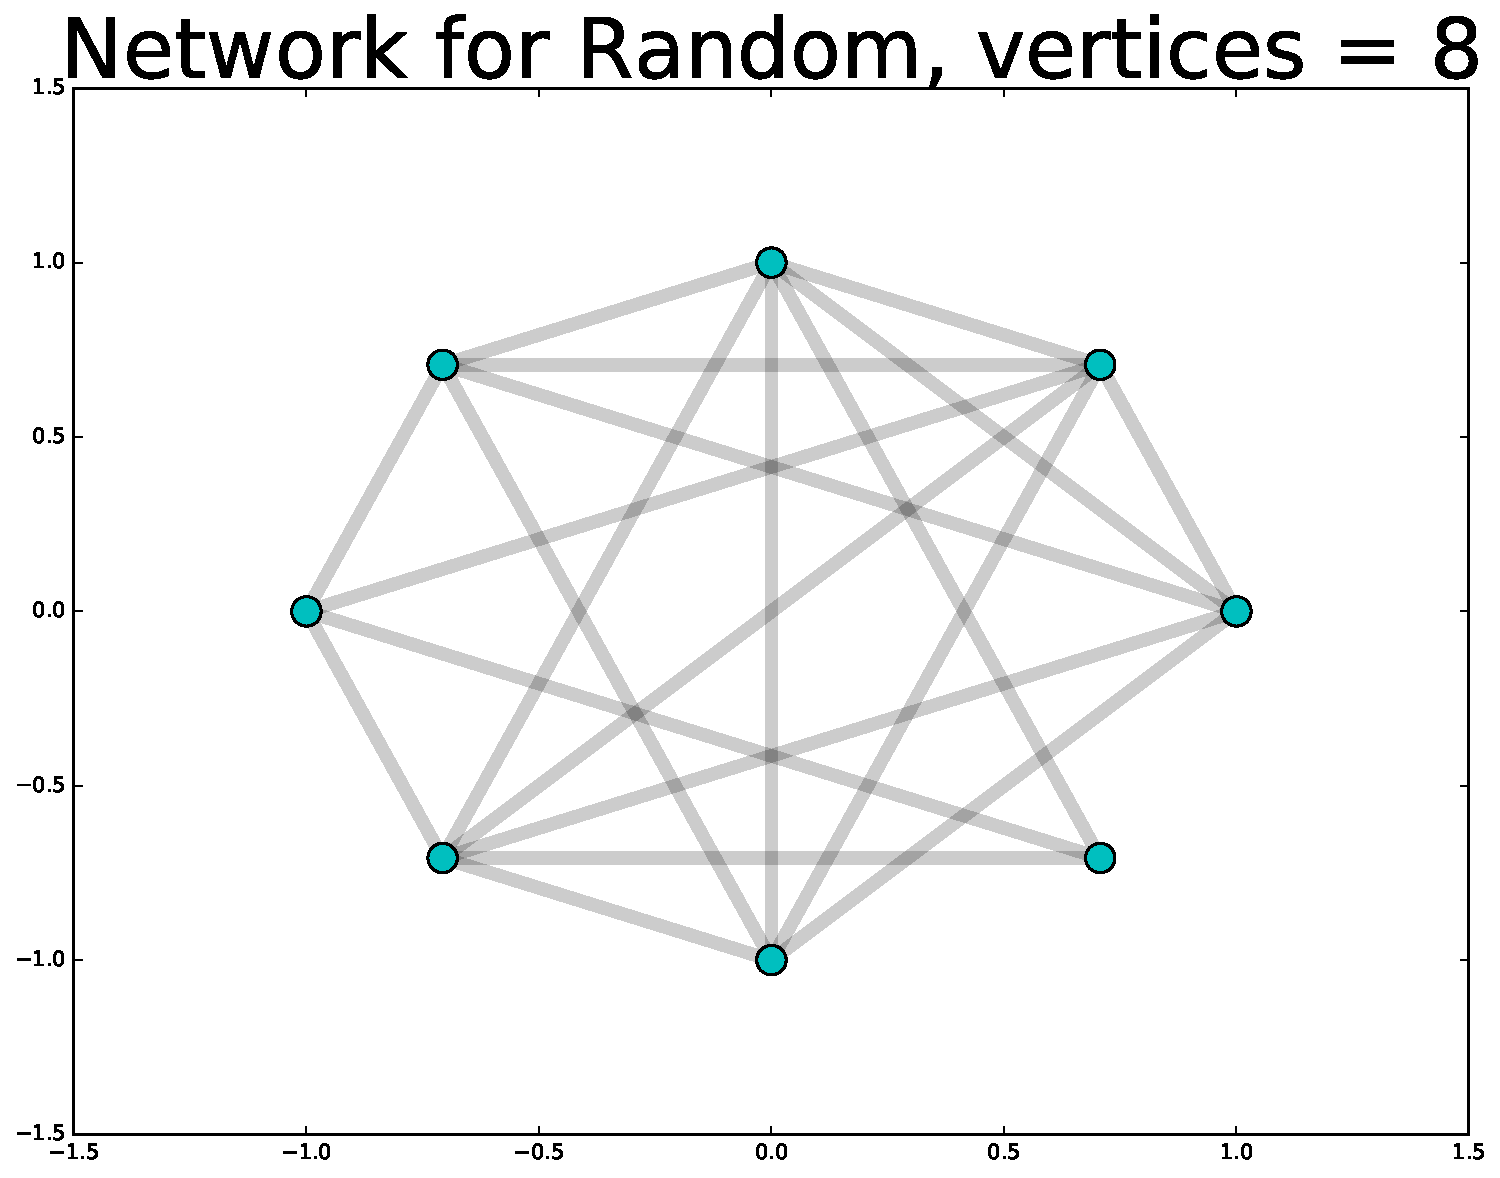
\includegraphics[width=\linewidth]{chapter-four/random_8.pdf}
		\caption{Eight nodes.}
	\end{subfigure}
	\hfill
	\begin{subfigure}[t]{0.30\textwidth}\centering
		\centering
		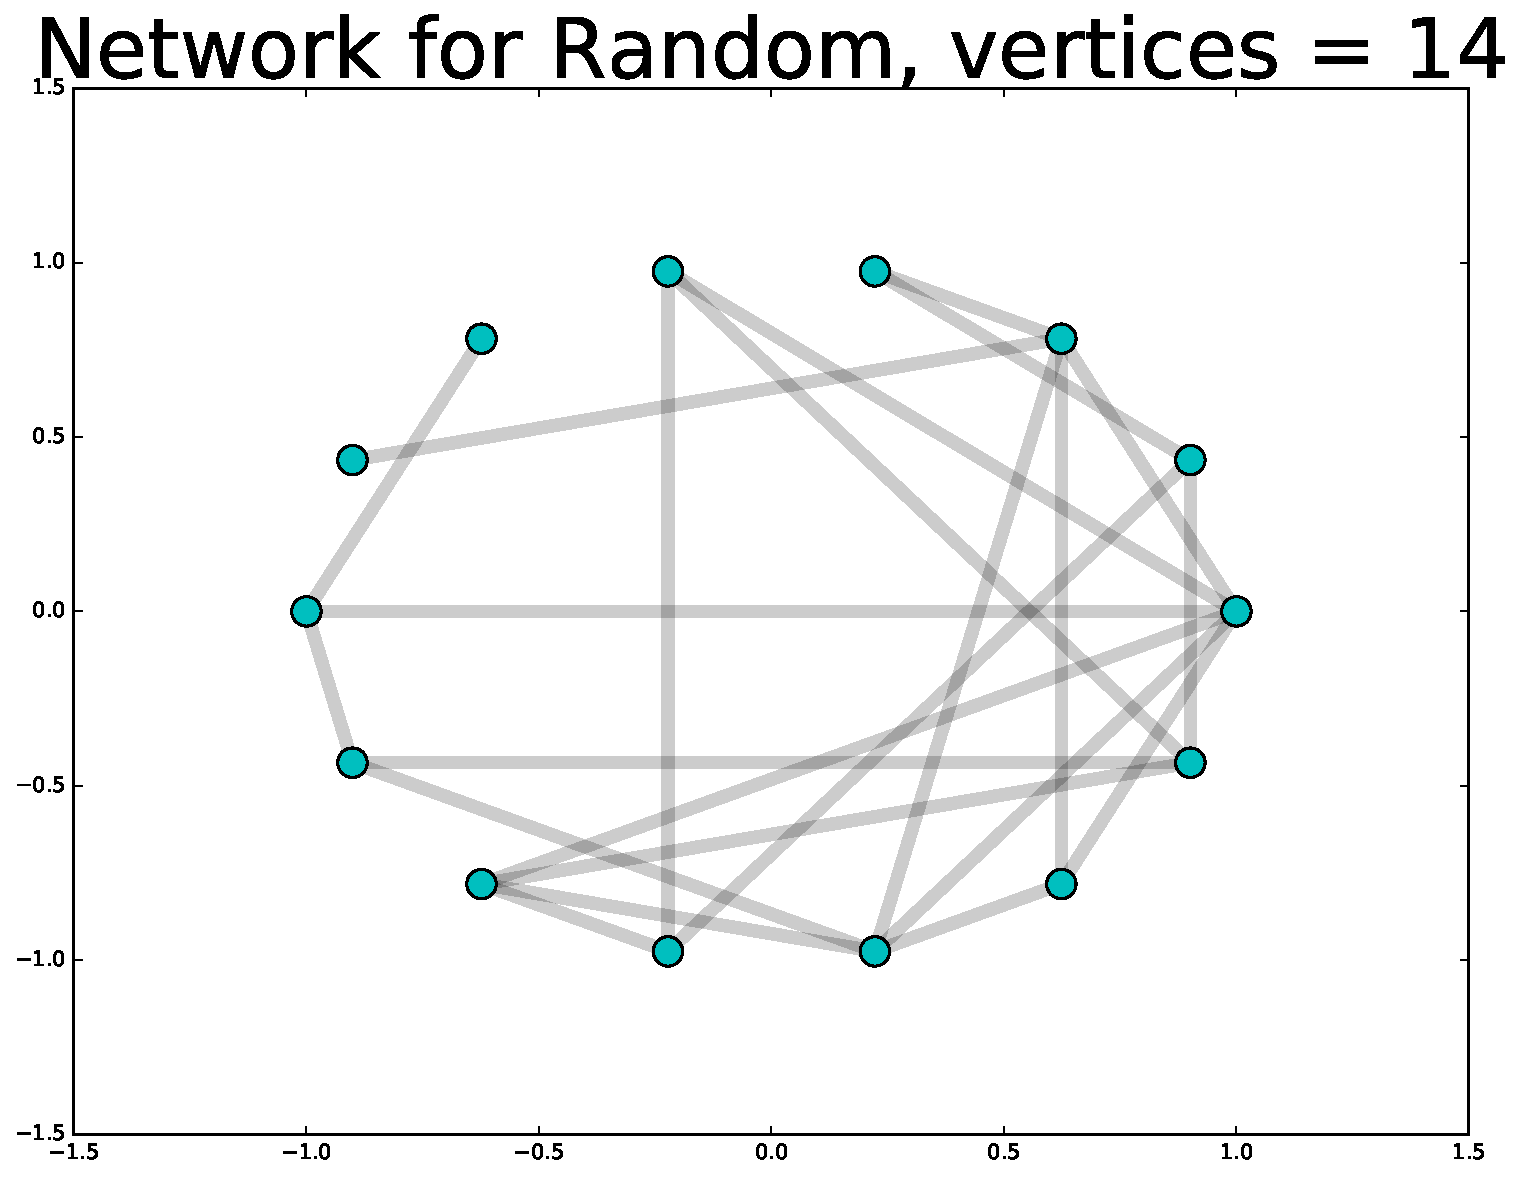
\includegraphics[width=\linewidth]{chapter-four/random_14.pdf}
		\caption{Fourteen nodes.}
	\end{subfigure}
	\hfill
	\begin{subfigure}[t]{0.30\textwidth}\centering
		\centering
		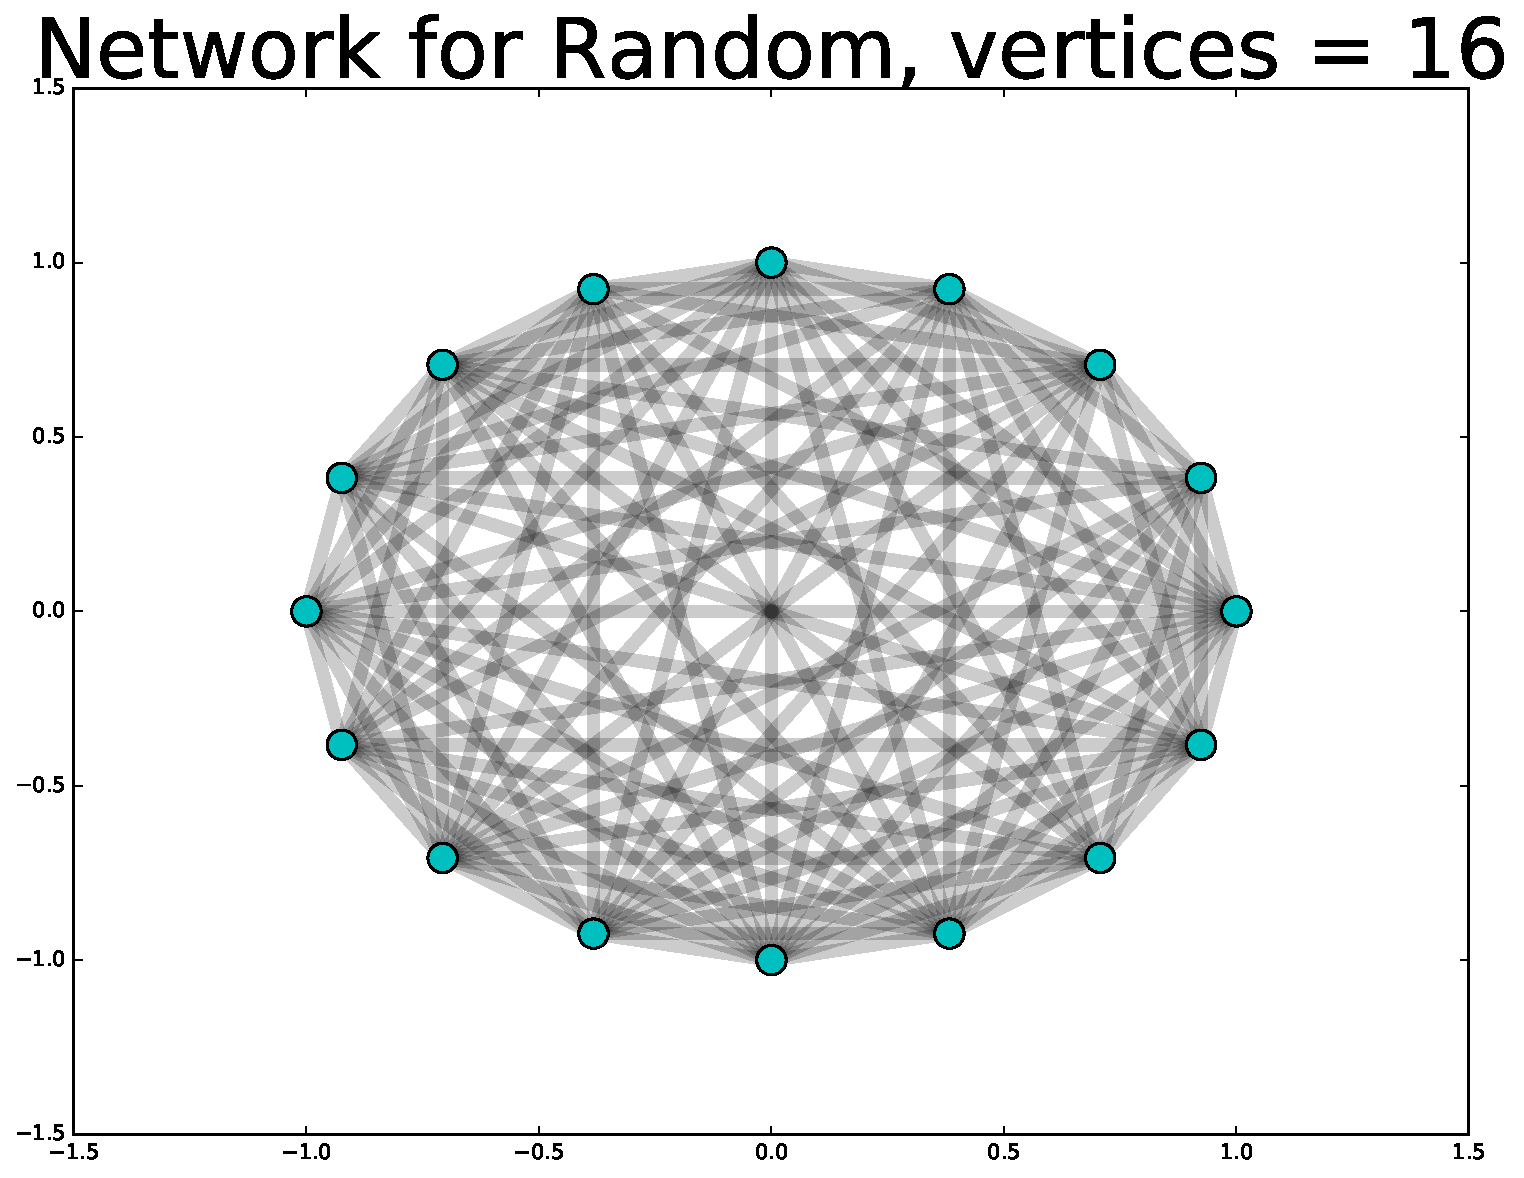
\includegraphics[width=\linewidth]{chapter-four/random_16.pdf}
		\caption{Sixteen nodes.}
	\end{subfigure}
	\hfill
	\begin{subfigure}[t]{0.30\textwidth}\centering
		\centering
		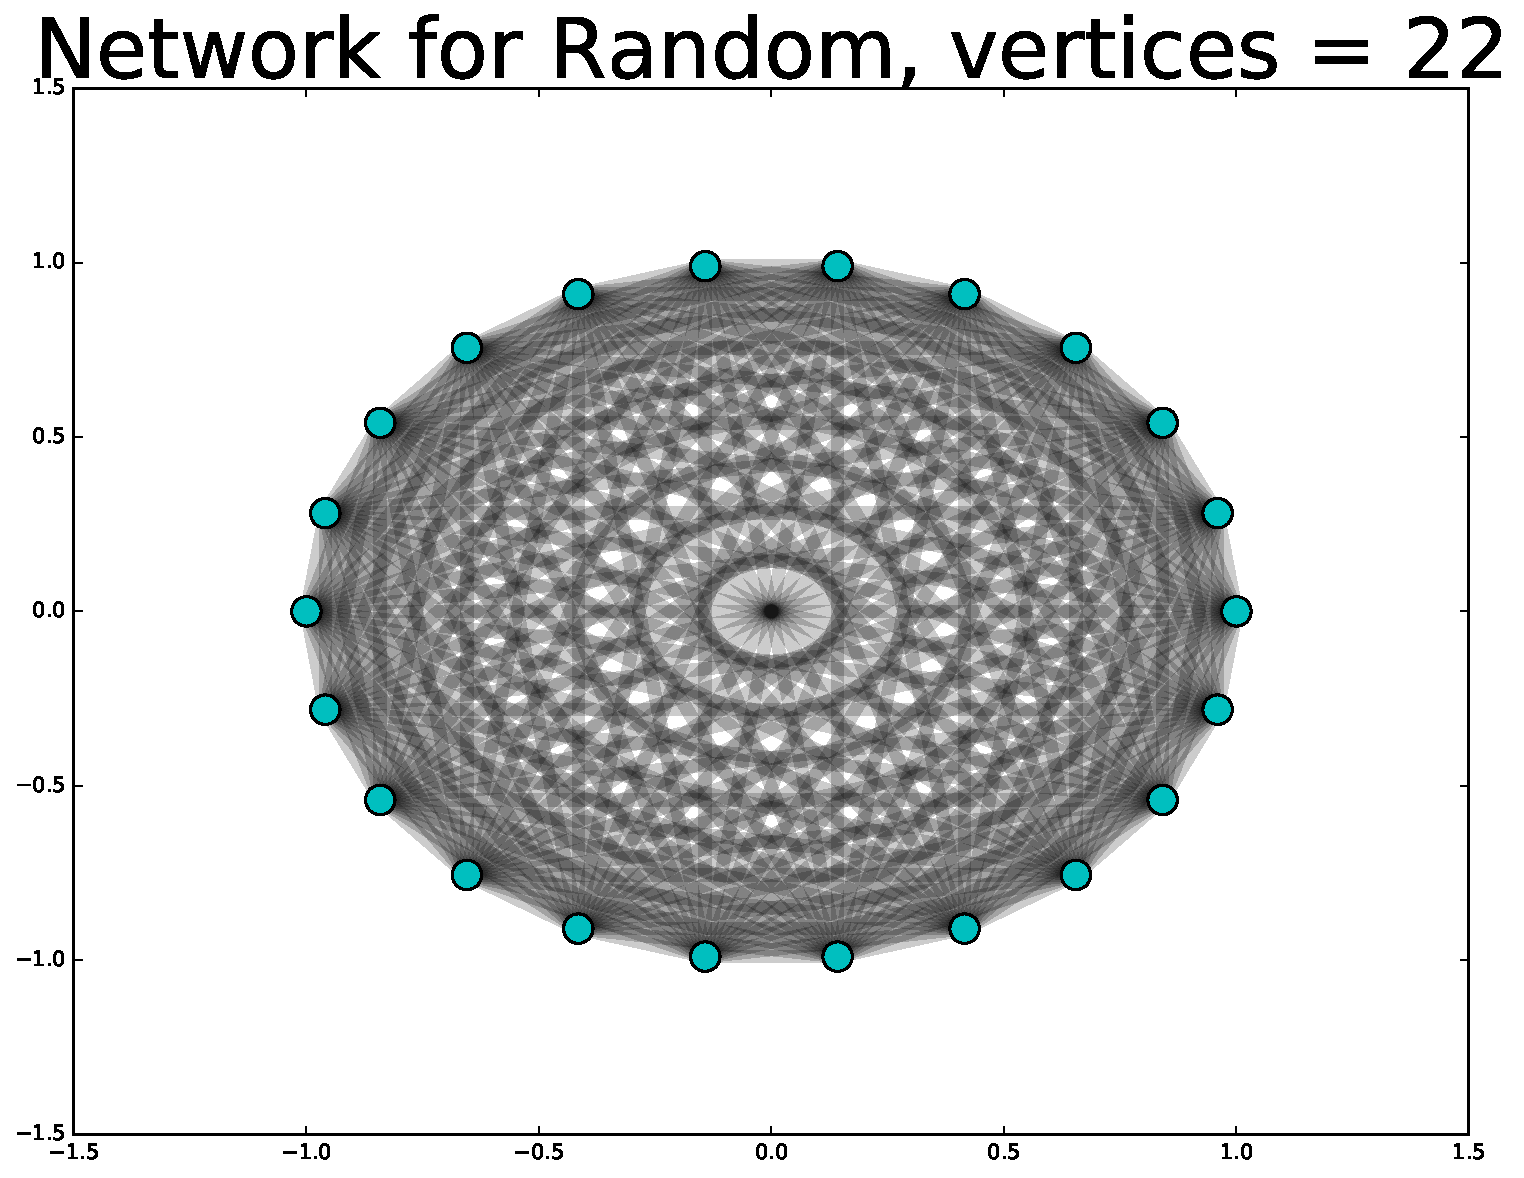
\includegraphics[width=\linewidth]{chapter-four/random_22.pdf}
		\caption{Twenty-two nodes.}
	\end{subfigure}
	\caption{Various Erd\"{o}s R\'{e}nyi networks.}
	\label{random_networks_illustration}
\end{figure}

Lastly, the complete networks experiment, was the only experiment where the
tournament size ranges from 2 to 50. A total of 500 networks, with complete topology,
have been constructed and played through. Table ~\ref{complete-summary-table}
summarizes, a few of the networks measures. For the complete networks, the measures
could have been predicted, due to the 'all connected rule'. The connectivity
coefficient it is equal to the degree. They vary from 1 to 49. One degree value
corresponds to the first network, with a minimum number of nodes 2, and 49 to
the last networks, with a maximum number of 50 nodes.

\begin{table}[!hbtp]
	\centering
	\begin{adjustbox}{width=0.6\textwidth}
		\small
		\begin{tabular}{|l|l|l|l|l|}
			\hline
			\multicolumn{5}{|c|}{Complete Networks Summary Table}                     \\ \hline
			     & connectivity & clustering & degree & nodes                  \\ \hline
			mean & 32.70        & 0.99       & 32.70  & 33.70                  \\ \hline
			std  & 11.87        & 0.03       & 11.87  & \multicolumn{1}{c|}{-} \\ \hline
			min  & 1.00         & 0.00       & 1.00   & 2.00                   \\ \hline
			max  & 49.00        & 1.00       & 49.00  & 50.00                  \\ \hline
		\end{tabular}
	\end{adjustbox}
	\caption{Complete Summary Table}
	\label{complete-summary-table}
\end{table}

The mean clustering coefficients is set at 0.99 Indicating strong clusters
throughout the experiment, an anticipated result. Furthermore, eight random
graphs are displayed in~\ref{complete_networks_illustration}.

\begin{figure}[!hbtp]
	\centering
	\begin{subfigure}[t]{0.30\textwidth}
		\centering
		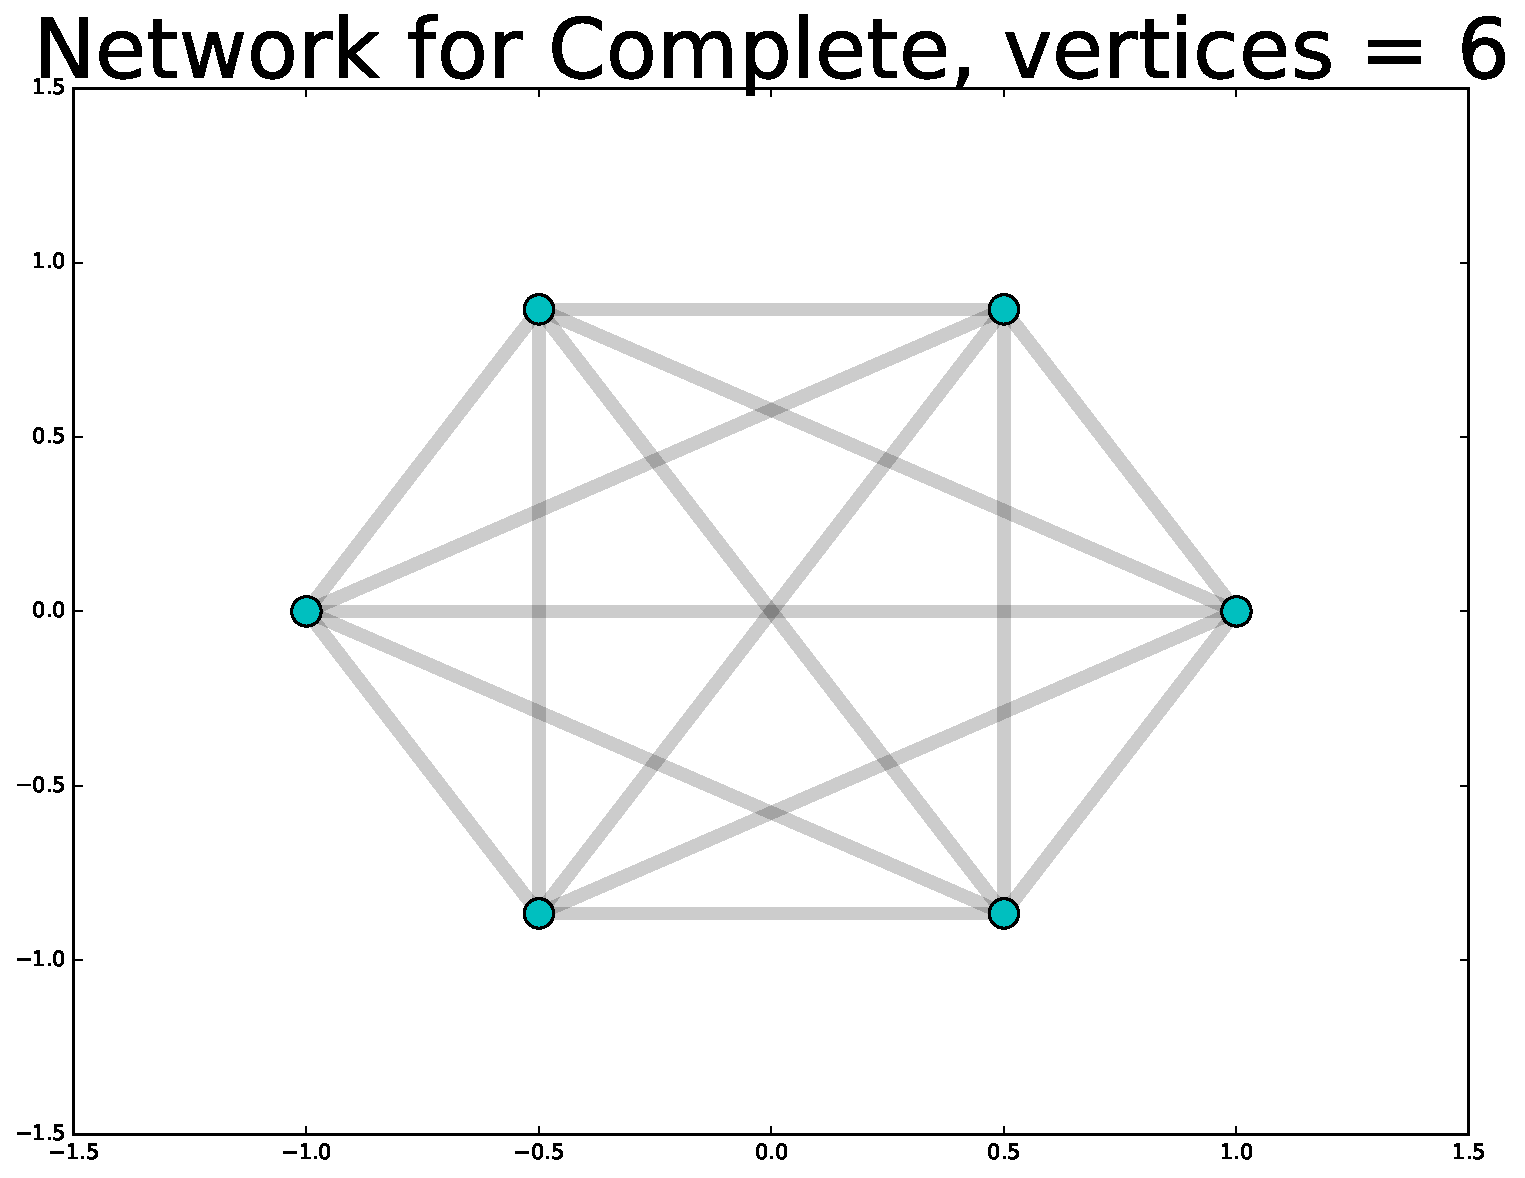
\includegraphics[width=\linewidth]{chapter-four/complete_6.pdf}
		\caption{Six nodes.}
	\end{subfigure}
	\hfill
	\begin{subfigure}[t]{0.30\textwidth}\centering
		\centering
		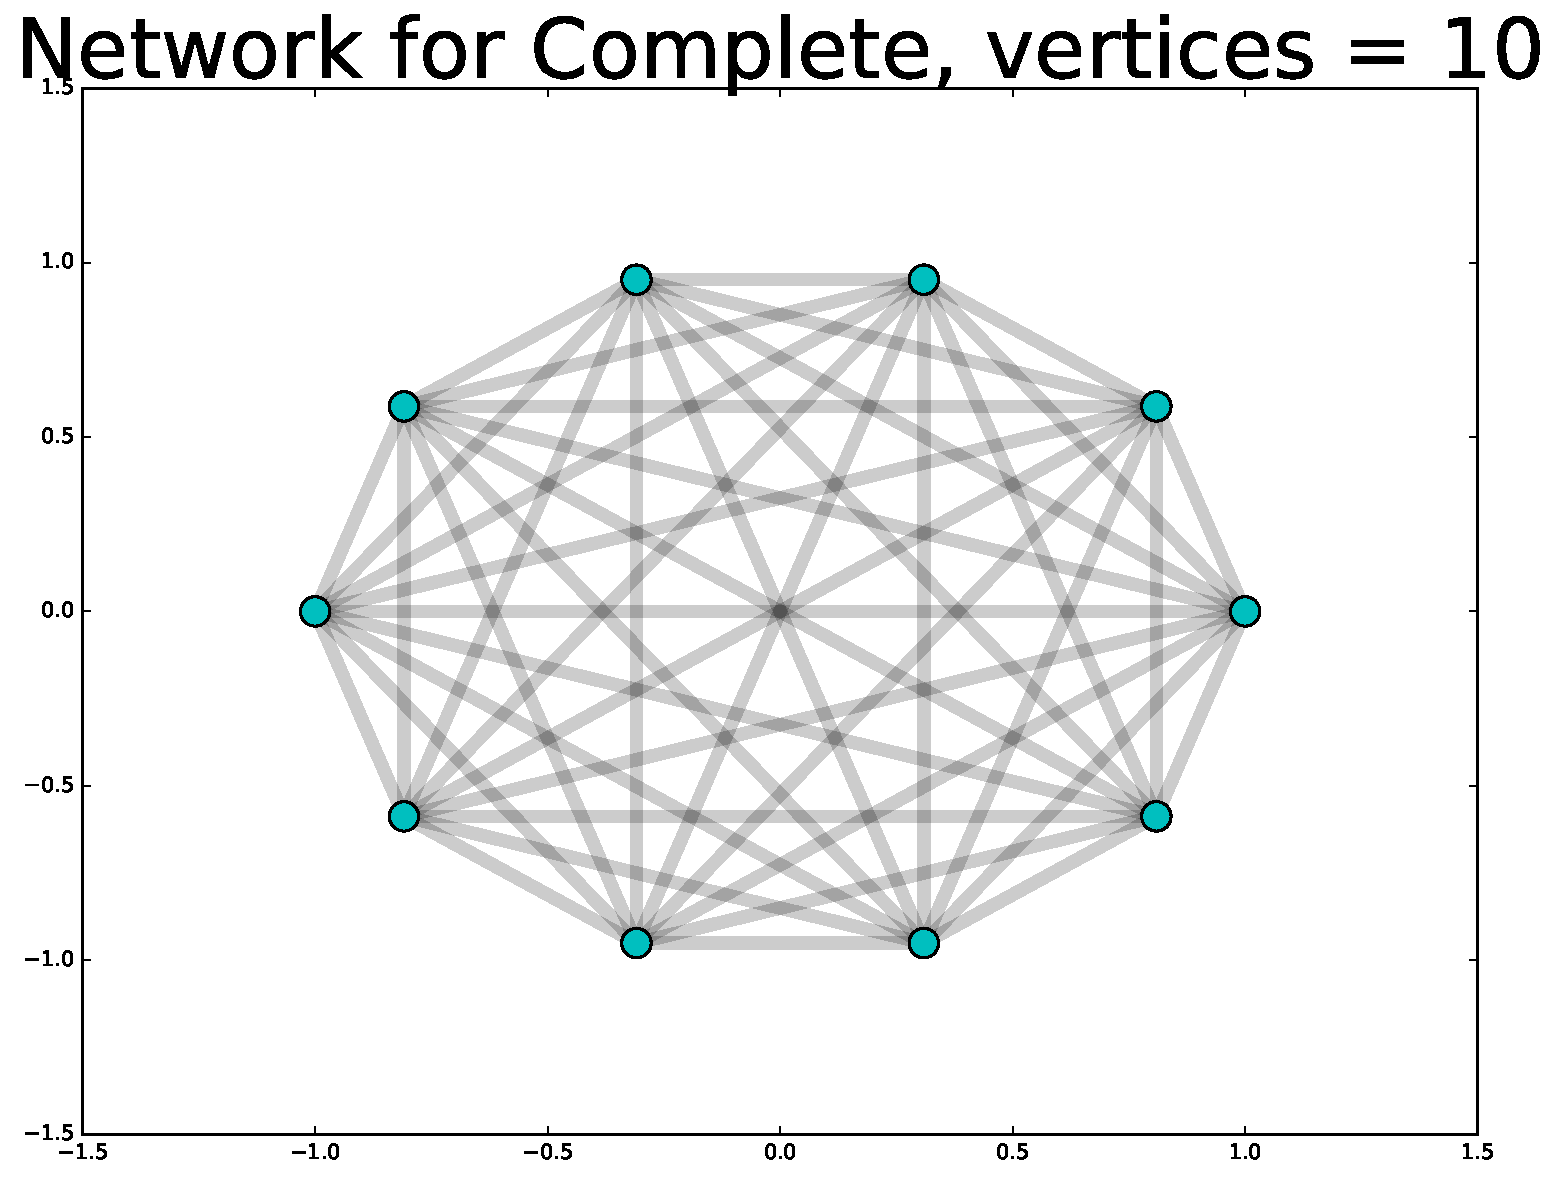
\includegraphics[width=\linewidth]{chapter-four/complete_10.pdf}
		\caption{Ten nodes.}
	\end{subfigure}
	\hfill
	\begin{subfigure}[t]{0.30\textwidth}\centering
		\centering
		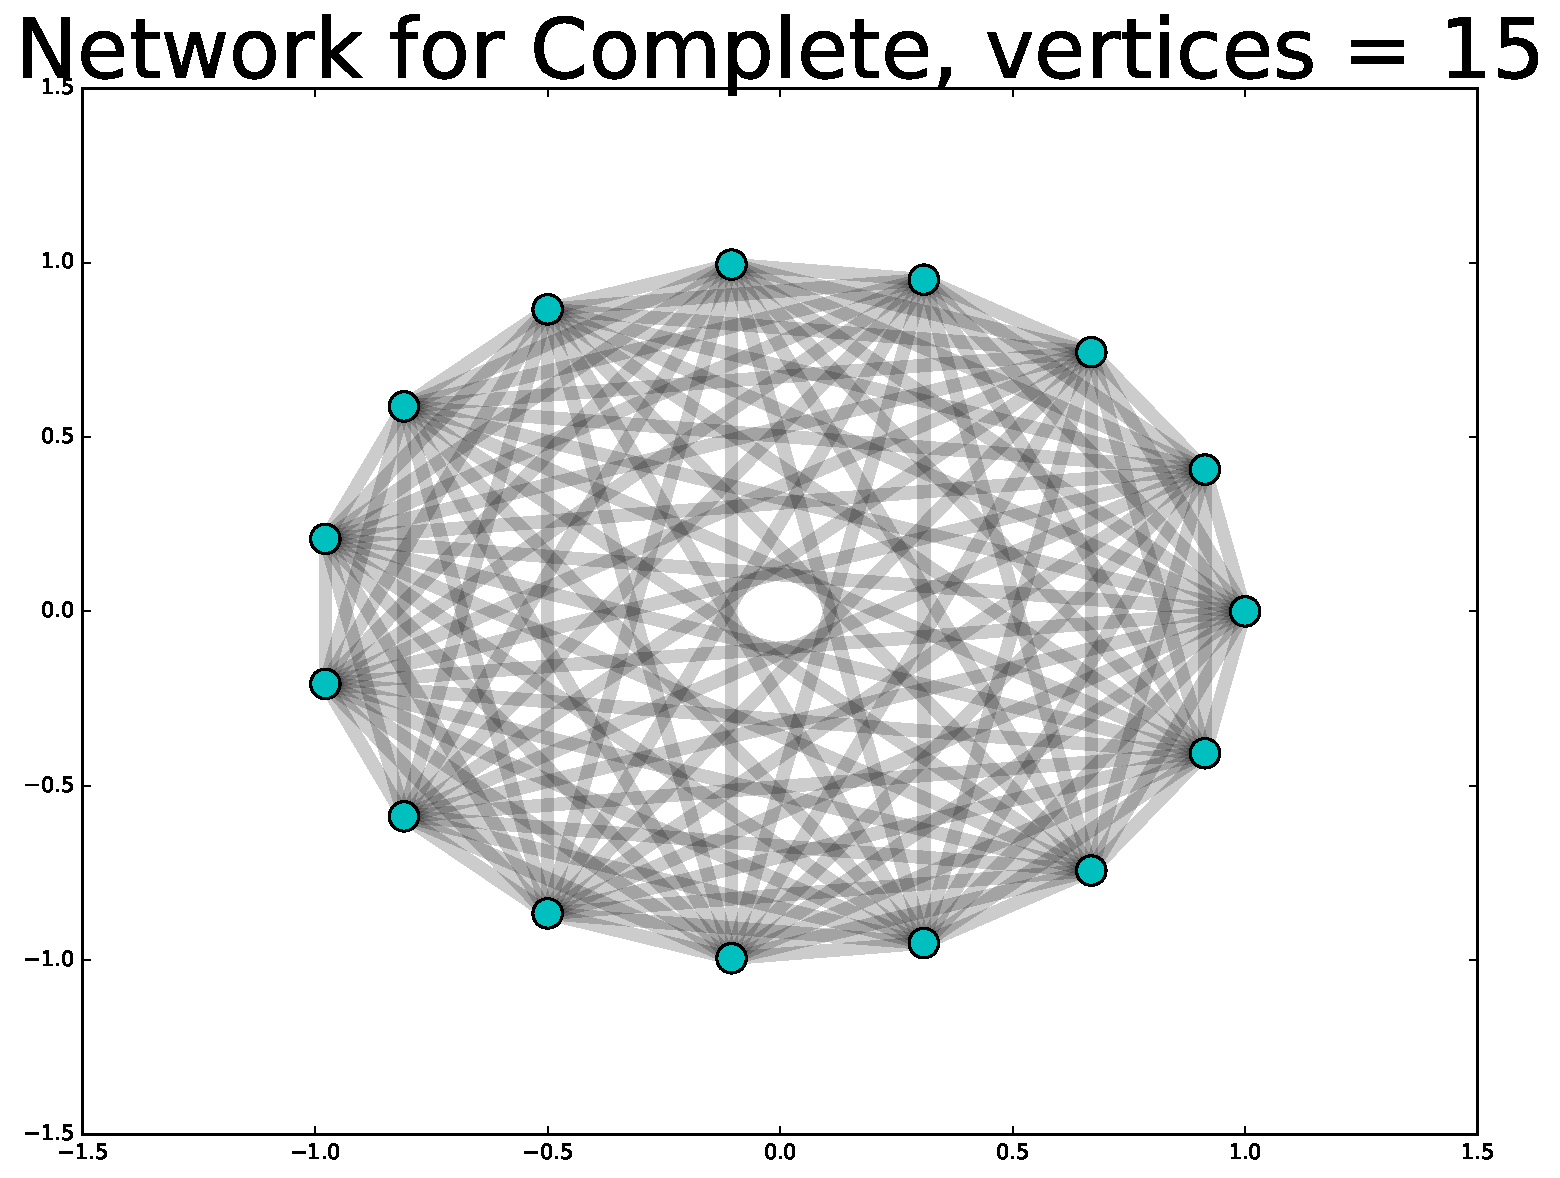
\includegraphics[width=\linewidth]{chapter-four/complete_15.pdf}
		\caption{Fifteen nodes.}
	\end{subfigure}
	\hfill
	\begin{subfigure}[t]{0.30\textwidth}\centering
		\centering
		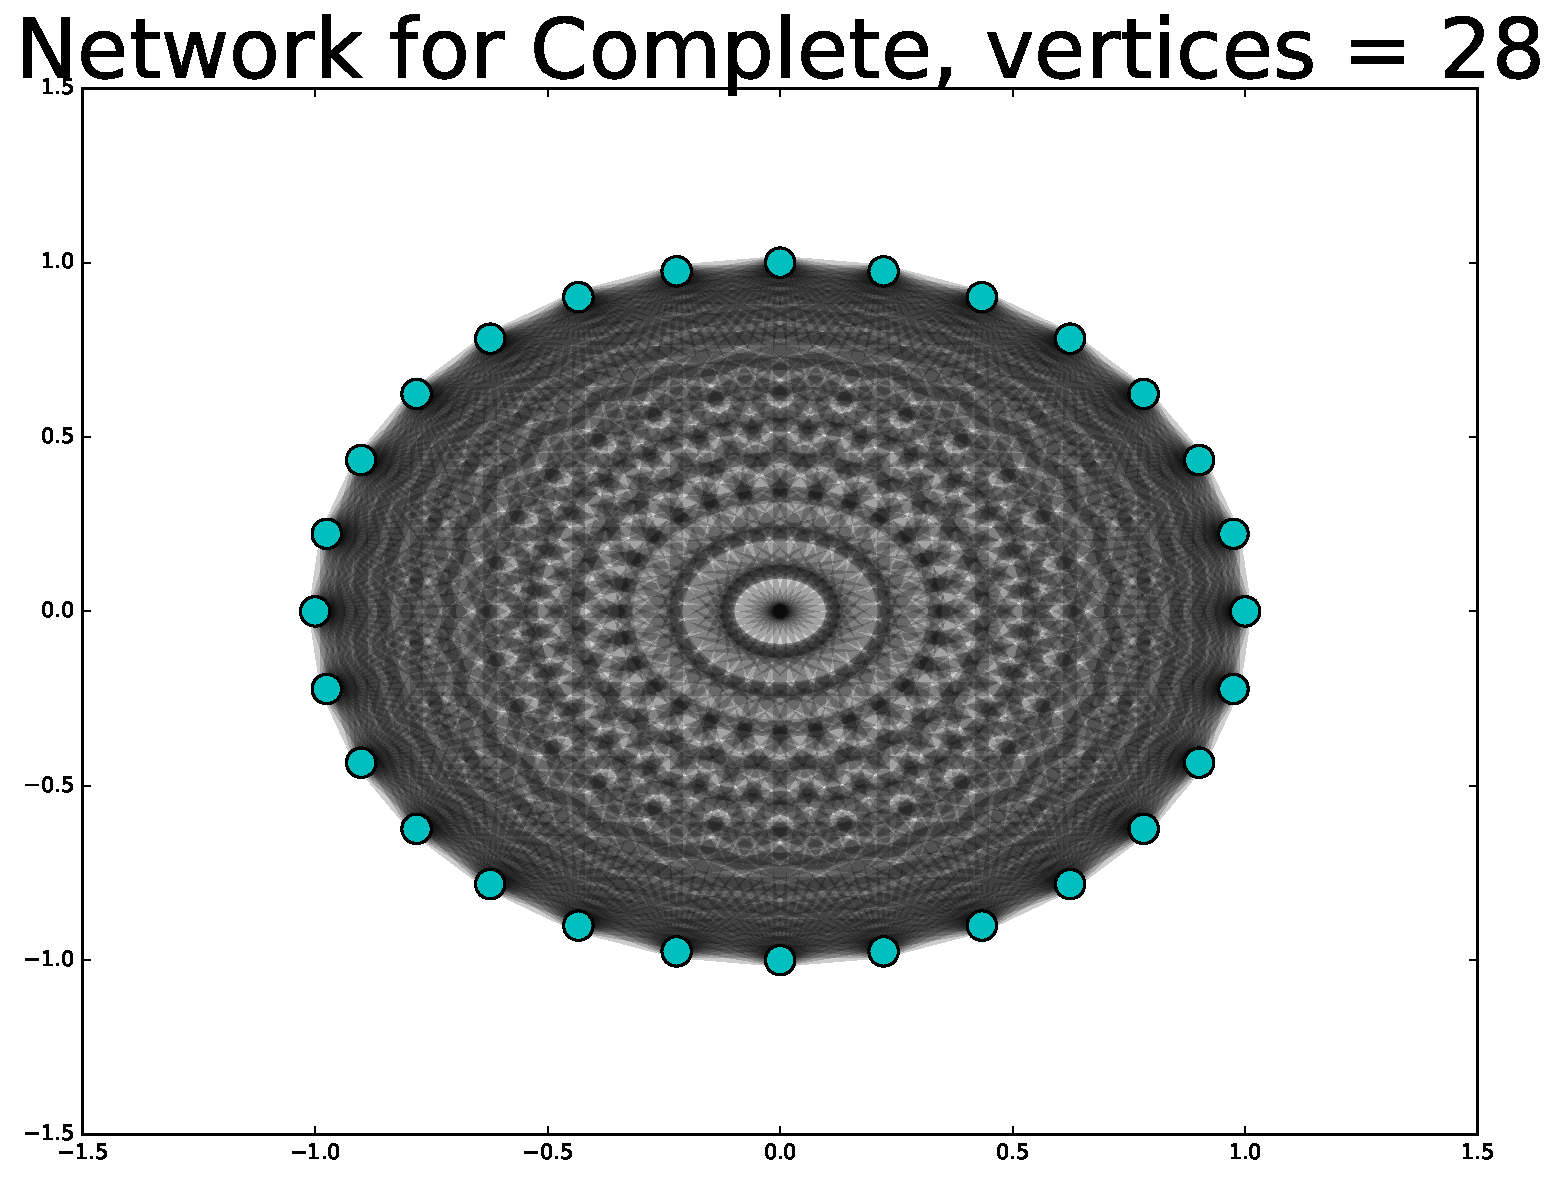
\includegraphics[width=\linewidth]{chapter-four/complete_28.pdf}
		\caption{Twenty-eight nodes.}
	\end{subfigure}
	\hfill
	\begin{subfigure}[t]{0.30\textwidth}\centering
		\centering
		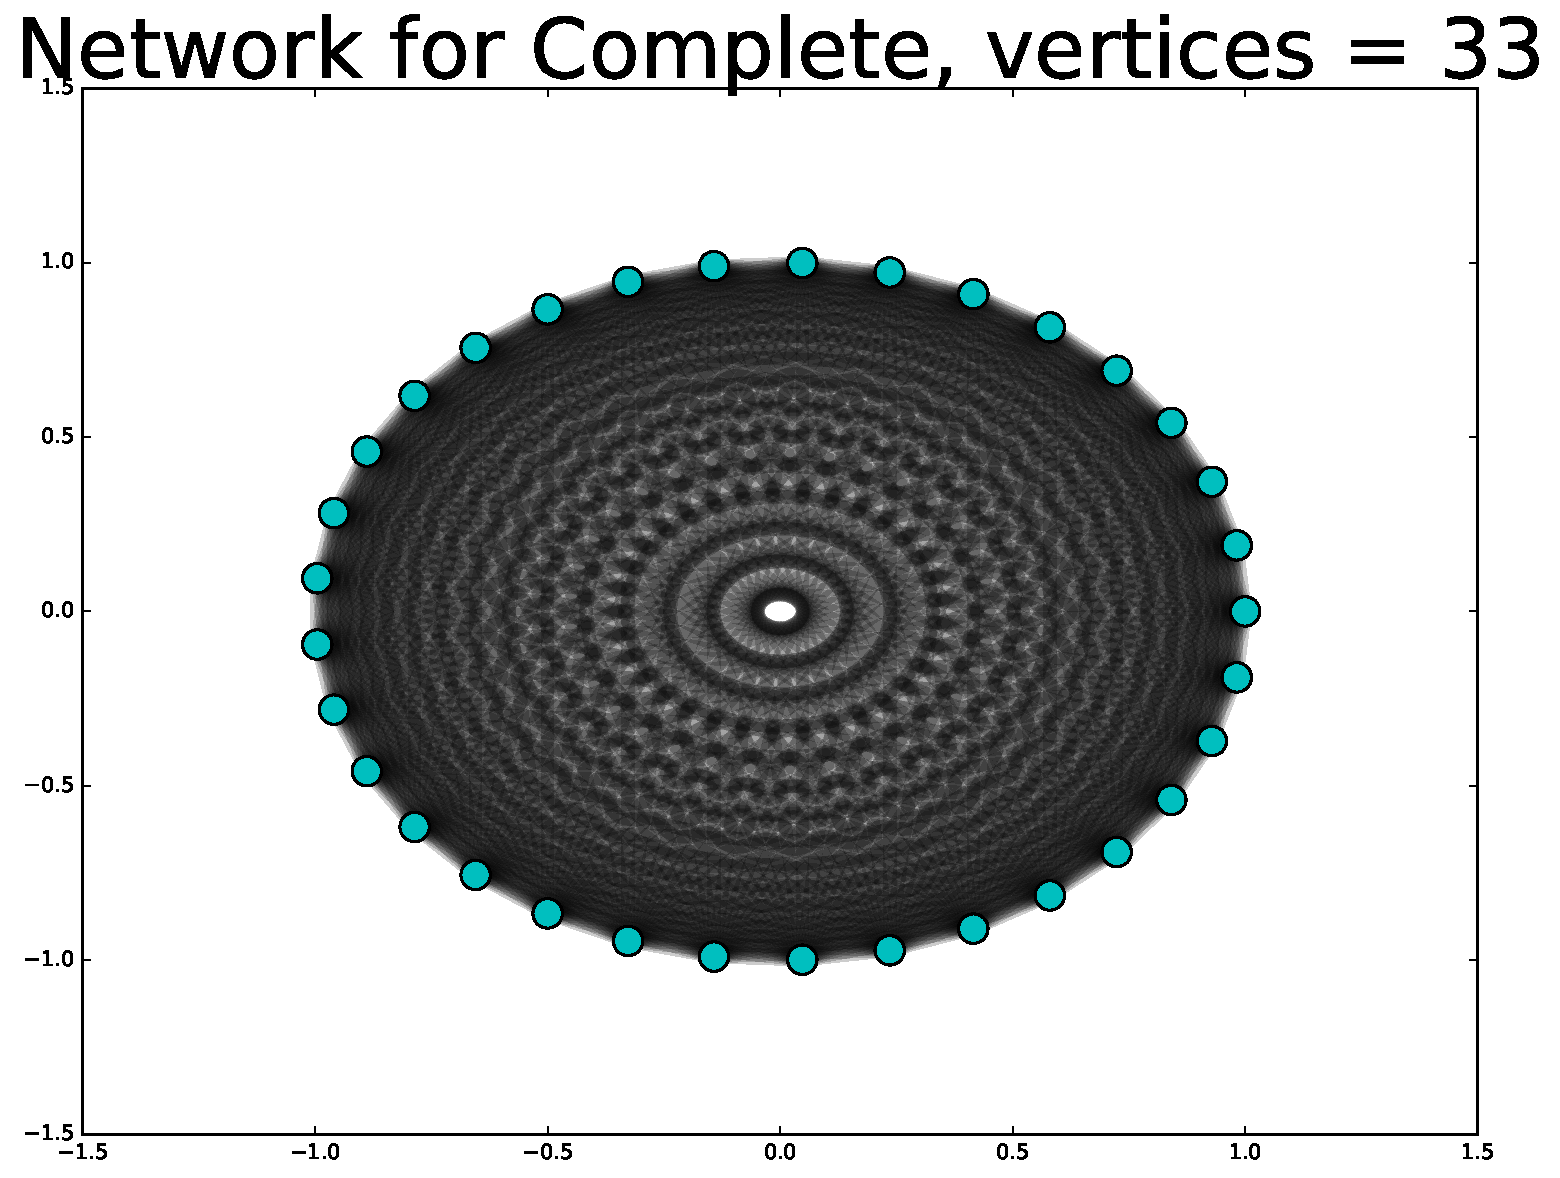
\includegraphics[width=\linewidth]{chapter-four/complete_33.pdf}
		\caption{Thirty-three nodes.}
	\end{subfigure}
	\hfill
	\begin{subfigure}[t]{0.30\textwidth}\centering
		\centering
		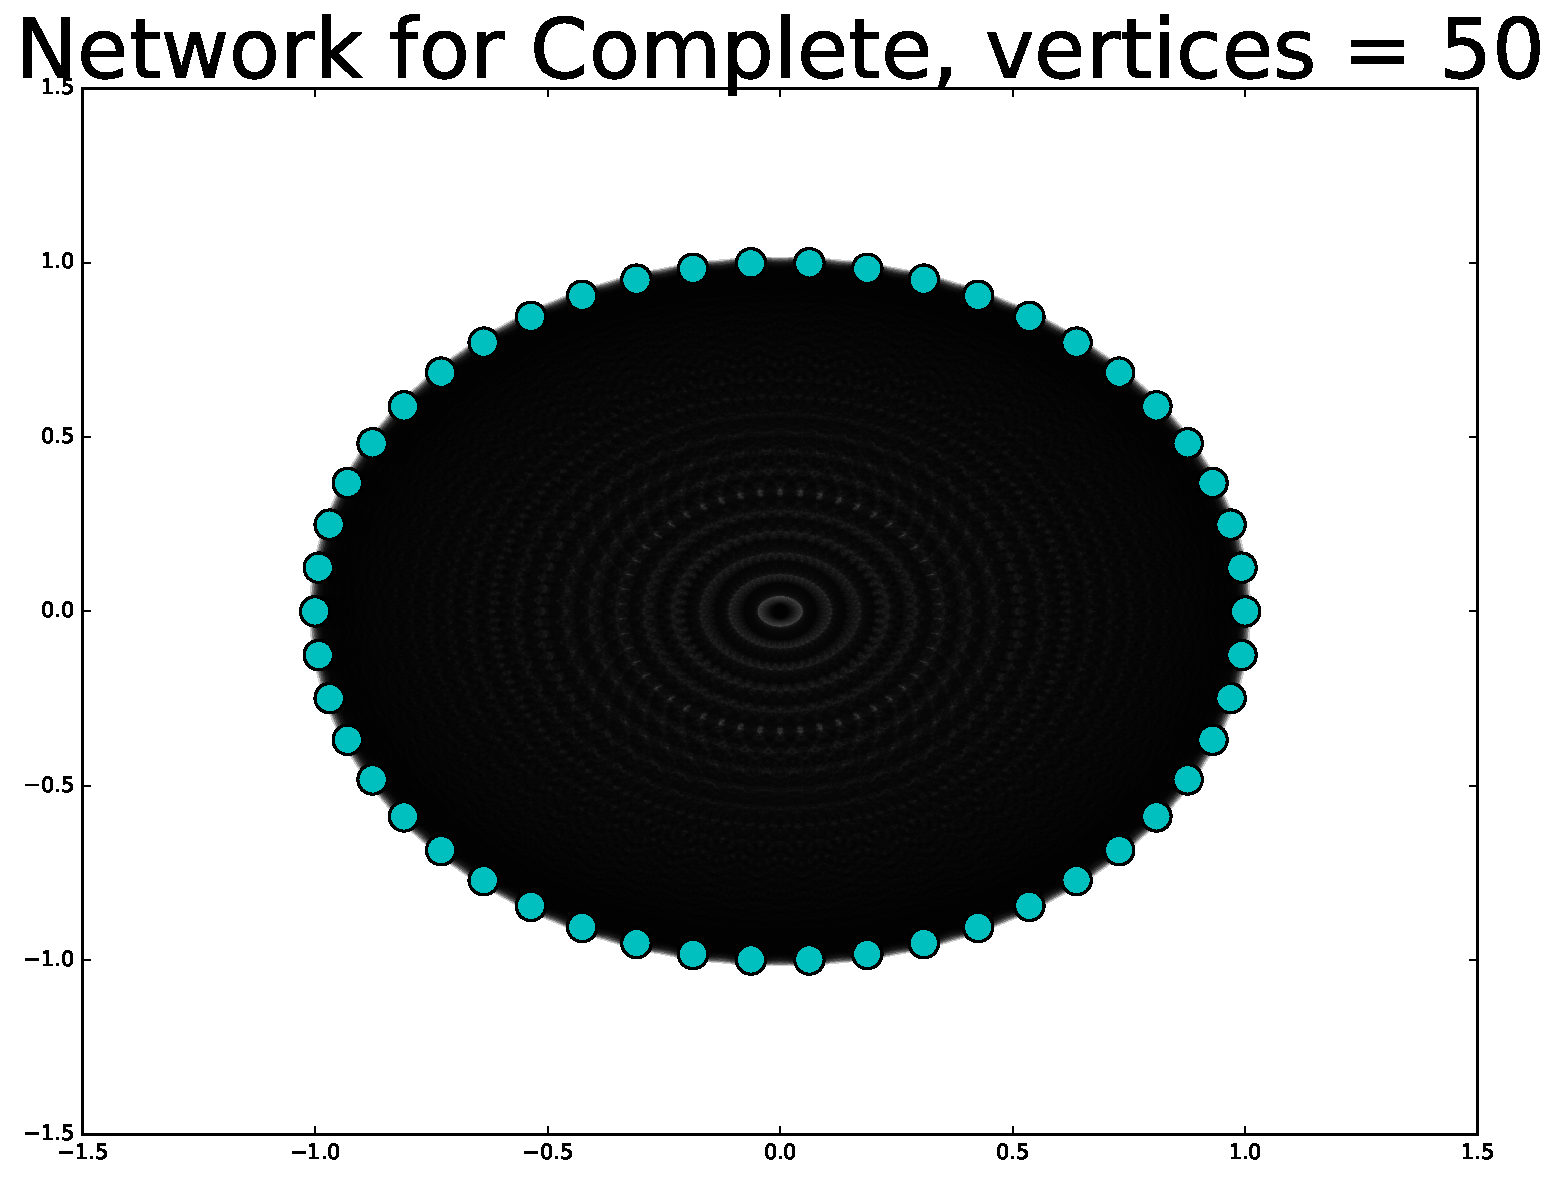
\includegraphics[width=\linewidth]{chapter-four/complete_50.pdf}
		\caption{FIfty nodes.}
	\end{subfigure}
	\caption{Various Complete networks.}
	\label{complete_networks_illustration}
\end{figure}

In this subsection, an initial summary of the overall graphs conducted, in
each of the experiment has been held. The number of tournaments, as well as the
tournament size differ. That is not a negative fact, what has been tried to
achieved in the complex networks experiments, is more complex and random
networks. In the following subsection, an initial analysis on the data produced
by these experiments in held.

\subsection{Data Analysis}

This subsection summarizes the data that have been extracted for the experiments.
Individual tables have been managed for each topology. The payoff matrix, for
the game of the prisoners dilemmas, follows the payoffs as explained in~\ref{sub:prisoner-dilemma}.
Thus, punishment payoff is equal to 1 temptation to 5, reward is equal to 3 and
the sucker's payoff is set to 0.

For the small word, Watts Strogratx, experiment the description of the
average score, average neighborhood score, cooperating ratio and neighborhood
size are shown in~\ref{summary-small-data}. The average score and average
neighborhood score, are fairly equal, both ranging form 0 to 5 with an average of
2.4. This could indicate that all strategies performed similarly. The mean
cooperation rating, is equal to 0.64. Thus, strategies behave mostly cooperative.
Mean neighborhood size is 4, agrees with~\ref{sub:network-analysis}.
Maximum neighbors is 9, so even if the maximum players has been 11, non strategy
compete against 10 strategies.

\begin{table}[!hbtp]
	\centering
	\begin{adjustbox}{width=0.8\textwidth}
		\small
		\begin{tabular}{|l|l|l|l|l|}
			\hline
			\multicolumn{5}{|c|}{Small world Data Summary Table}                                \\ \hline
			     & average score & average neighborhood & cooperating ratio & neighborhood size \\ \hline
			mean & 2.40          & 2.40                 & 0.64              & 4.74              \\ \hline
			std  & 0.63          & 0.40                 & 0.30              & 2.65              \\ \hline
			min  & 0.00          & 0.00                 & 0.00              & 1.00              \\ \hline
			max  & 5.00          & 5.00                 & 1.00              & 12.00             \\ \hline
		\end{tabular}
	\end{adjustbox}
	\caption{Small world Data Summary Table}
	\label{summary-small-data}
\end{table}

For the random, Erd\"{o}s R\'{e}nyi, Table ~\ref{summary-random-data}, is
an initial summary, for basic measure of the experiment. Similarly, the average score and average
neighborhood score, are fairly equal. This time, the average neighborhood score,
is slightly lower, 2.38, and the maximum average score achieved by a strategy
is 4.99. Instead of the maximum of a 5. The mean cooperating ration, is higher
than 0.50 again. Thus, strategies tend to cooperate and the neighborhood size,
verifies the results of ~\ref{sub:network-analysis}.

\begin{table}[!hbtp]
	\centering
	\begin{adjustbox}{width=0.8\textwidth}
		\small
		\begin{tabular}{|l|l|l|l|l|}
			\hline
			\multicolumn{5}{|c|}{Random Data Summary Table}                                      \\ \hline
			     & average score & average neighborhood & cooperating ratio & neighborhood size \\ \hline
			mean & 2.38          & 2.38                 & 0.63              & 11.00             \\ \hline
			std  & 0.48          & 0.24                 & 0.25              & 6.57              \\ \hline
			min  & 0.00          & 0.00                 & 0.00              & 1.00              \\ \hline
			max  & 5.00          & 4.99                 & 1.00              & 28.00             \\ \hline
		\end{tabular}
	\end{adjustbox}
	\caption{Random Data Summary Table}
	\label{summary-random-data}
\end{table}

Finally, for the complete experiment, Table ~\ref{summary-complete-data}. The
average scores, are lower for this experiment. Both mean average scores are
equal to 2.38. But the maximum average scores, strategies and neighbors, are
below 4. On the other hand, the minimum score are non zero. The behavior of the
scores can be explained by the topology. Complete experiment, is the experiment
with highest number of games played. Considering that for each tournament
\(n-1\) games take place. Thus, scoring zero is less possible, because the games
you play are increased by far, and the overall score falls, because of the number
of the opponents.
Cooperating ratio, is similarly once again and the neighborhood size
verify what was discussed in ~\ref{sub:network-analysis}.

\begin{table}[!hbtp]
	\centering
	\begin{adjustbox}{width=0.8\textwidth}
		\small
		\begin{tabular}{|l|l|l|l|l|}
			\hline
			\multicolumn{5}{|c|}{Complete Data Summary Table}                                      \\ \hline
			     & average score & average neighborhood & cooperating ratio & neighborhood size \\ \hline
			mean & 2.38          & 2.38                 & 0.63              & 32.70             \\ \hline
			std  & 0.13          & 0.35                 & 0.23              & 11.90             \\ \hline
			min  & 0.54          & 0.55                 & 0.00              & 1.00              \\ \hline
			max  & 3.58          & 3.89                 & 1.00              & 49.00             \\ \hline
		\end{tabular}
	\end{adjustbox}
	\caption{Complete Data Summary Table}
	\label{summary-complete-data}
\end{table}

In this subsection, a very brief summary was done to the data. In the section
to follow, more important topics will be raised and an analysis of the best
ranking strategies will take place.

\subsection{Classification}
\label{sub:four-classification}
As stated in [], the Axelrod-Python library (version 1.16.00), consists of 132.
Reading though the documentation for each strategy, enough to be able to
understand and distinguish, any similarities between their player, would be an
unbearable task. Even so, another concept provided by the Axelrod- Python library
is the cooperating ratio. The cooperating ratio, is the ratio of times
a strategy cooperated, divided by the number of turns in a single tournament.

Initially the data of all experiments have been combined, and afterwards have been
grouped by each strategy. The average cooperating ratio for each strategy is then
computed. Furthermore, by using the \(k\)-means algorithm, the boundaries for
any given number of categories can be found. For the cooperation, five individual
categories have been chosen. The lowest category representing the non - cooperative
strategies, the middle category, the medium cooperatives and the highest
the cooperative ones. The two remaining categories, represent the
moderate and weak cooperation strategies respectively.

The results, for performing the algorithm, in each experiment can seen in Tables,
~\ref{class} and a more detailed table, with the respective category of each
strategy can be found in the Appendix~\ref{append:class-categories}.

Overall six strategies are in the low category. Their average cooperating ration
ranges between 0.00 and 0.20. In the weak category, the ratio is between
0.23 and 0.40, and is consisted by 17 strategies. Twenty-eight strategies are
in the mid category, with upper bound of ratio 0.57 and lower bound a 0.42.
The moderate category, is for strategies which ratio is between 0.58 and 0.75.
Lastly, the high category, with 48 strategies and a mean ratio of 0.87.

\begin{table}[!hbtp]
	\centering
	\begin{adjustbox}{width=0.5\textwidth}
		\small
		\begin{tabular}{|l|l|l|l|l|}
			\hline
			\multicolumn{5}{|c|}{Classification Table}              \\ \hline
			Categories & count & \multicolumn{3}{l|}{cooperating ratio}        \\ \hline
			         &    & min  & mean & max  \\ \hline
			low      & 6  & 0.00 & 0.10 & 0.20 \\ \hline
			weak     & 17 & 0.23 & 0.32 & 0.40 \\ \hline
			mid      & 28 & 0.42 & 0.50 & 0.57 \\ \hline
			moderate & 33 & 0.58 & 0.65 & 0.75 \\ \hline
			high     & 48 & 0.76 & 0.87 & 1.00 \\ \hline
		\end{tabular}
	\end{adjustbox}
	\caption{Classification Table}
	\label{class}
\end{table}

The classification of the strategies will be a useful tool in the following
subsection. For now the categories have been introduced and more details, for
each strategy, can be found in the Appendix. This section have been for the
preliminarily analysis. Where an overview of the networks and data have been
conducted. In the section that follows, the analysis on performance is
undertaken.

\section{Performance Analysis}

In this section, three measure will be scrutinized, to assess performance of the
strategies. These measures are the winning ratio, the normalized average score
and the median rank. Various regression models have been constructed, for
the median rank and lastly, the findings are summarized.

As aforementioned, our experiments did not manage to achieve maximum capability.
Additionally, not all strategies participated in each of the experiments.
Even so, the goal of this chapter remains the observation of the strategies,
for any given topology. Thus, from here onwards the data that have been
used, are a combination of the data sets produced by each experiment. The
analysis is focused solidarily, on the overall performance of each strategy and
the identification of any network attributes, affecting the performance.

\subsection{Winning Ratio}

In this subsection, a ranking of the strategies has been carried out, based on
the winning ratio. Shown in Figure~\ref{wining-second-gen}, is a point plot illustrating the order
of the strategies based on this rank. The highest ranked strategies, are
Fool Me Forever, Grumpy, Ripoff, Cycler DDC and, with wining ratio
of 0.23 Calculator. Even though, Fool Me Forever, Grumpy, are overall cooperative
strategies Ripoff, Cycler DDC and Calcuter have a cooperative ratio around
0.35. It can be assumed that these strategies have been favored by their environment.

\begin{figure}[!hbtp]
	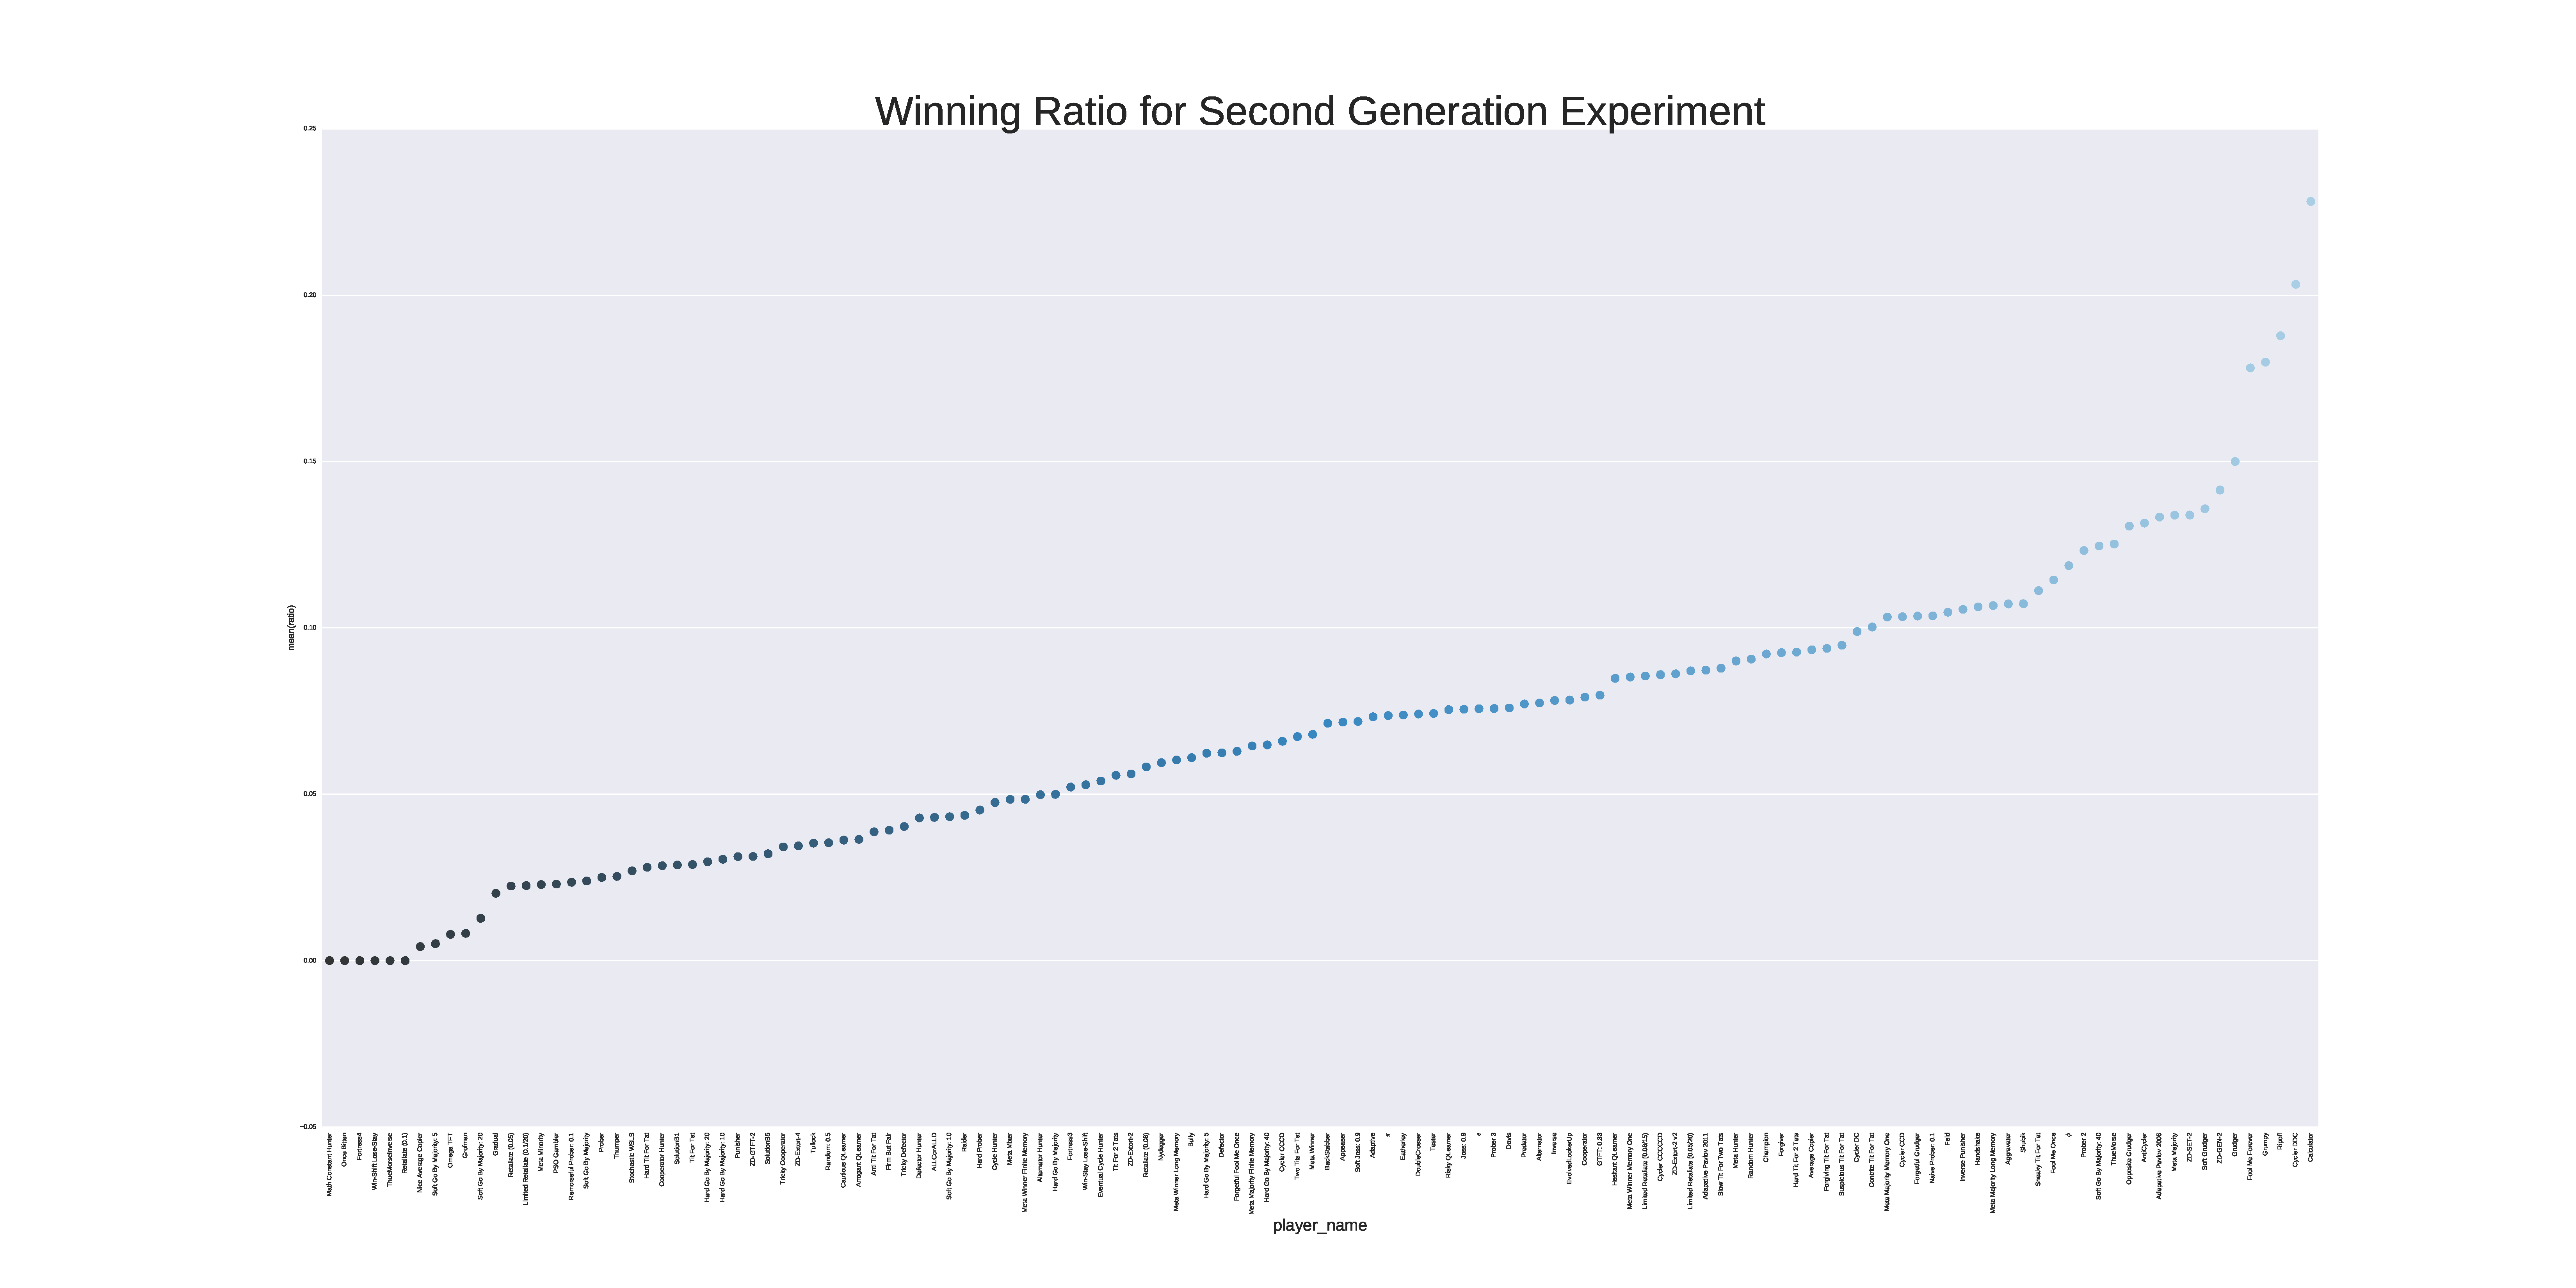
\includegraphics[width=1.2\linewidth,center]{chapter-four/winning-ratio.pdf}
	\caption{Winning Ratio Complex Networks Experiments}
	\label{wining-second-gen}
\end{figure}

Even so, by winning ratio it assumed that a well performed strategy, is a strategy
that have won. This raises questions as to, is the performance only based by that?
Is there any reassurance that this strategy did not stand 'lucky' in the small
number of tournaments that it had participated, because it was favored by
the circumstances and environment, and did not do poorly in the rest?
Thus, no more attention will be given to winning ratio, as it does not express
the overall well performance that is tried to be observed.

The following subsection, is focused on the normalized average score.

\subsection{Normalized Average Score}

In this subsection, an individual data frame for each strategy, with each of
their participations, is created.Thus, 132 frames. Therefore, by reading thought
these frames
the normalized average score is studied. To understand how the network topologies
affect the scoring of a strategy an Anova analysis has been executed.
To identify the effects of the topologies, the existence of a
statistically significant differences of the normalized score, between the
clustering and connectivity groups is being tested.

For the particular statistical analysis on this subsection, the scipy
python library is being used once again. Firstly, the normality of the average
score is being tested. By looping through the frames and using the scipy
command \texttt{scipy.stats.mstats.normaltest}, the tests are carried out quite simply.
The results indicate that for
each frame, all 132, the \(p\) value is lower than 0.05. Thus the average normalized
score is not normally distributed. For this reason, the Kruskal Wallis test, the
corresponding non parametric test, has been used.

For testing the difference between the connectivity groups, of each frame,
the following results have been returned. Most of the strategies, have a significant
difference in their scores. They returned a \(p\) value less than 0.05.
Thus, their scores have been affected by the connectivity  of the topology the
strategy played in. Even so, 45 strategies did not. These 45 strategies include,
Cycler DDC, Raider, Inverse Punisher, Hard Go By Majority and more. Randomly
chosen strategies, out of 132, have been chosen and the variation in their average
score is illustrated in the violin plots, in Figure~\ref{normalized-av-scr}:

\begin{figure}[!hbtp]
	\centering
	\begin{subfigure}[t]{0.70\textwidth}
		\centering
		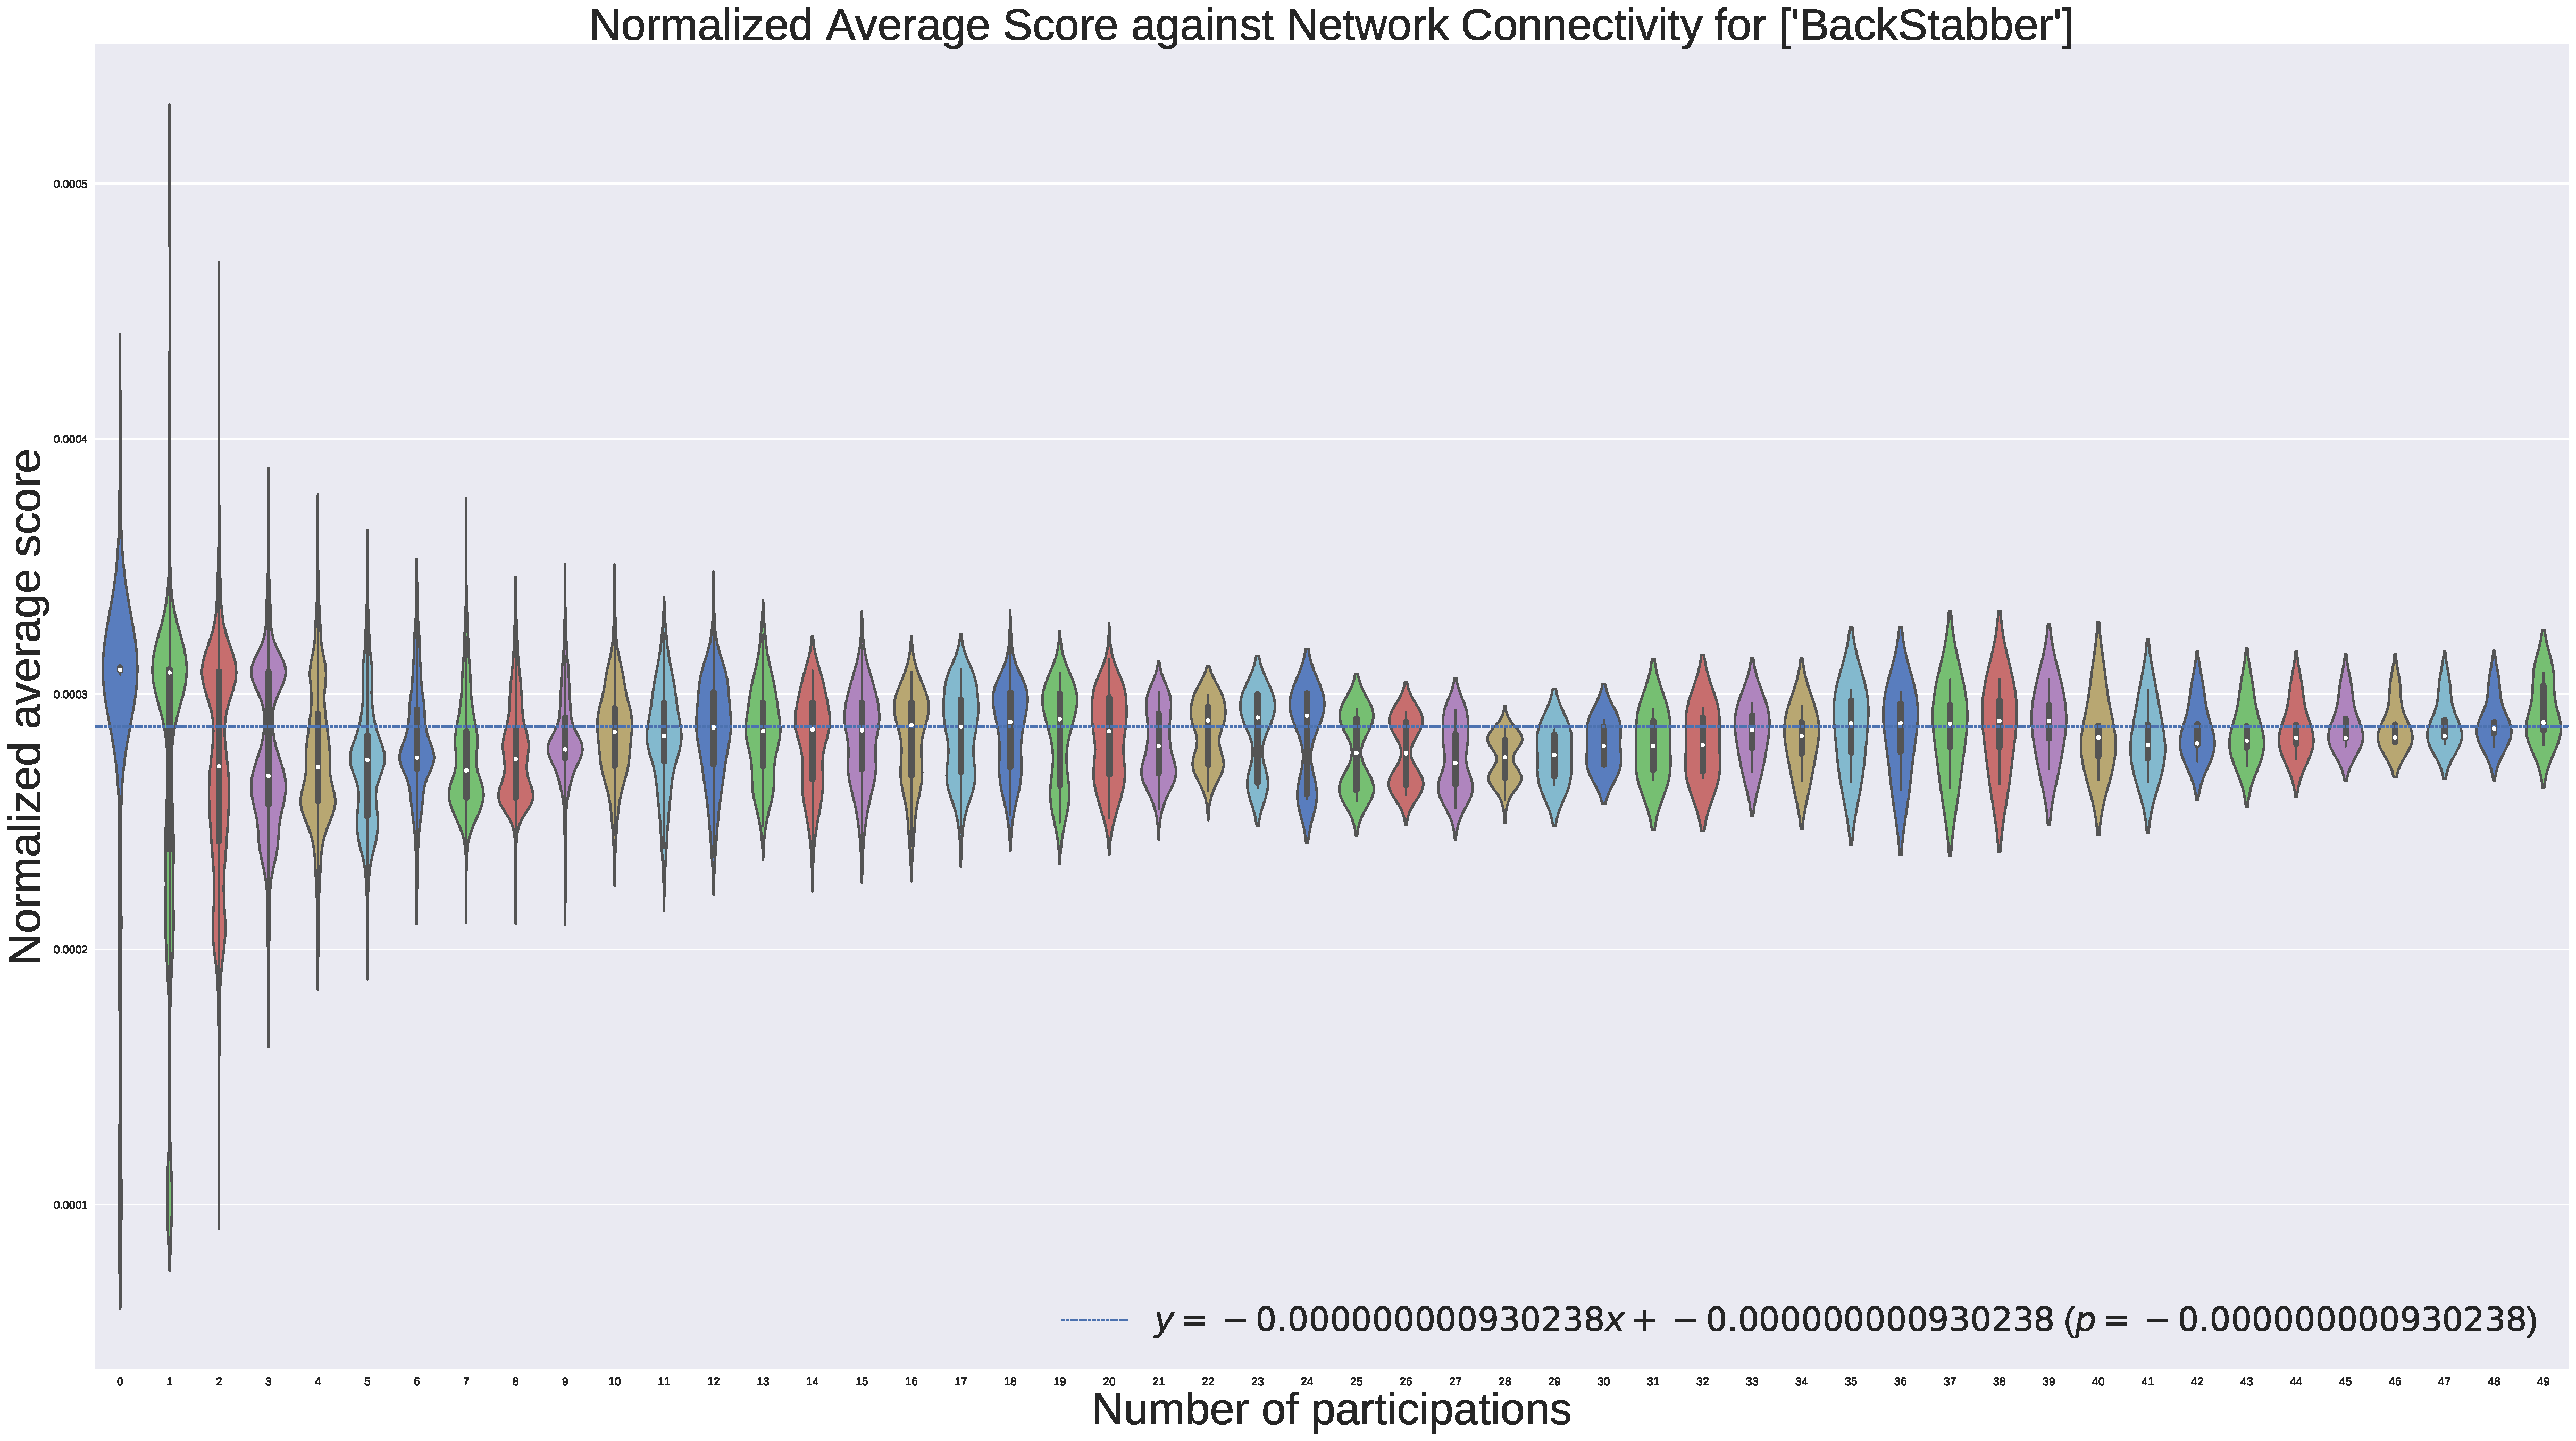
\includegraphics[width=\linewidth]{chapter-four/normalized-['BackStabber'].pdf}
		\caption{Normalized Average Score BackStabber}
	\end{subfigure}
	\hfill
	\begin{subfigure}[t]{0.70\textwidth}\centering
		\centering
		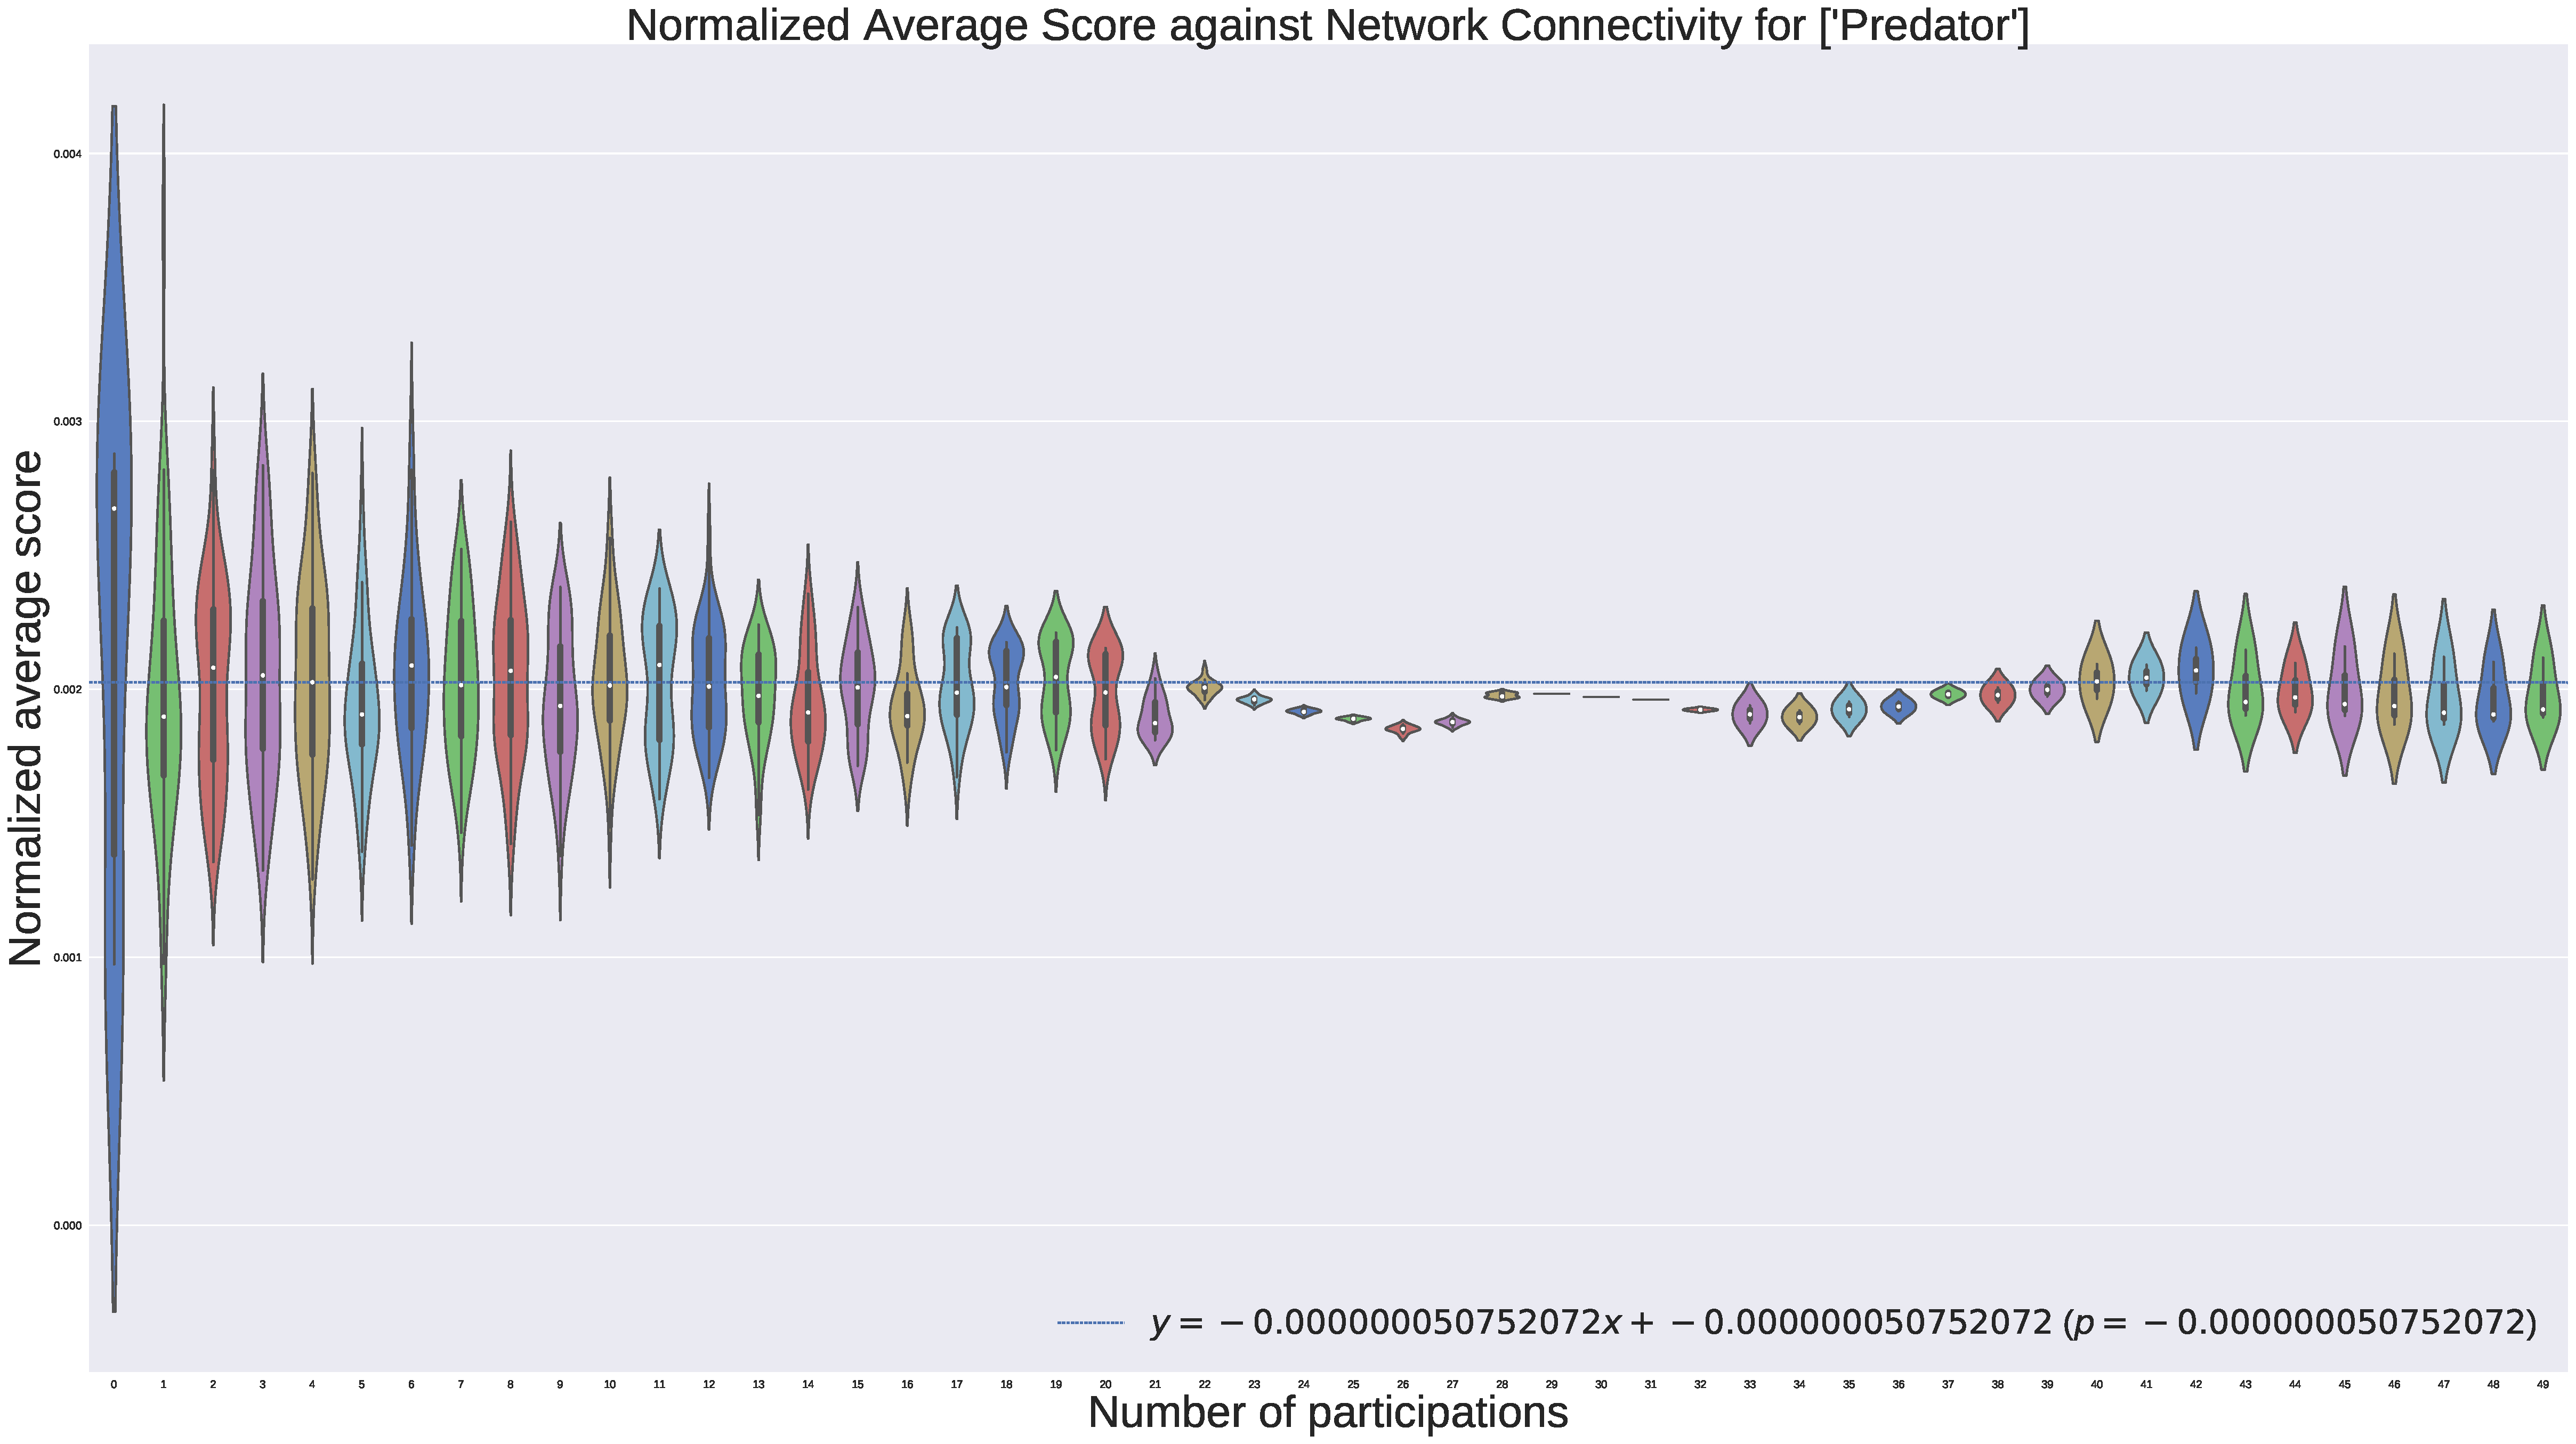
\includegraphics[width=\linewidth]{chapter-four/normalized-['Predator'].pdf}
		\caption{Normalized Average Score Predator}
	\end{subfigure}
	\hfill
	\begin{subfigure}[t]{0.70\textwidth}\centering
		\centering
		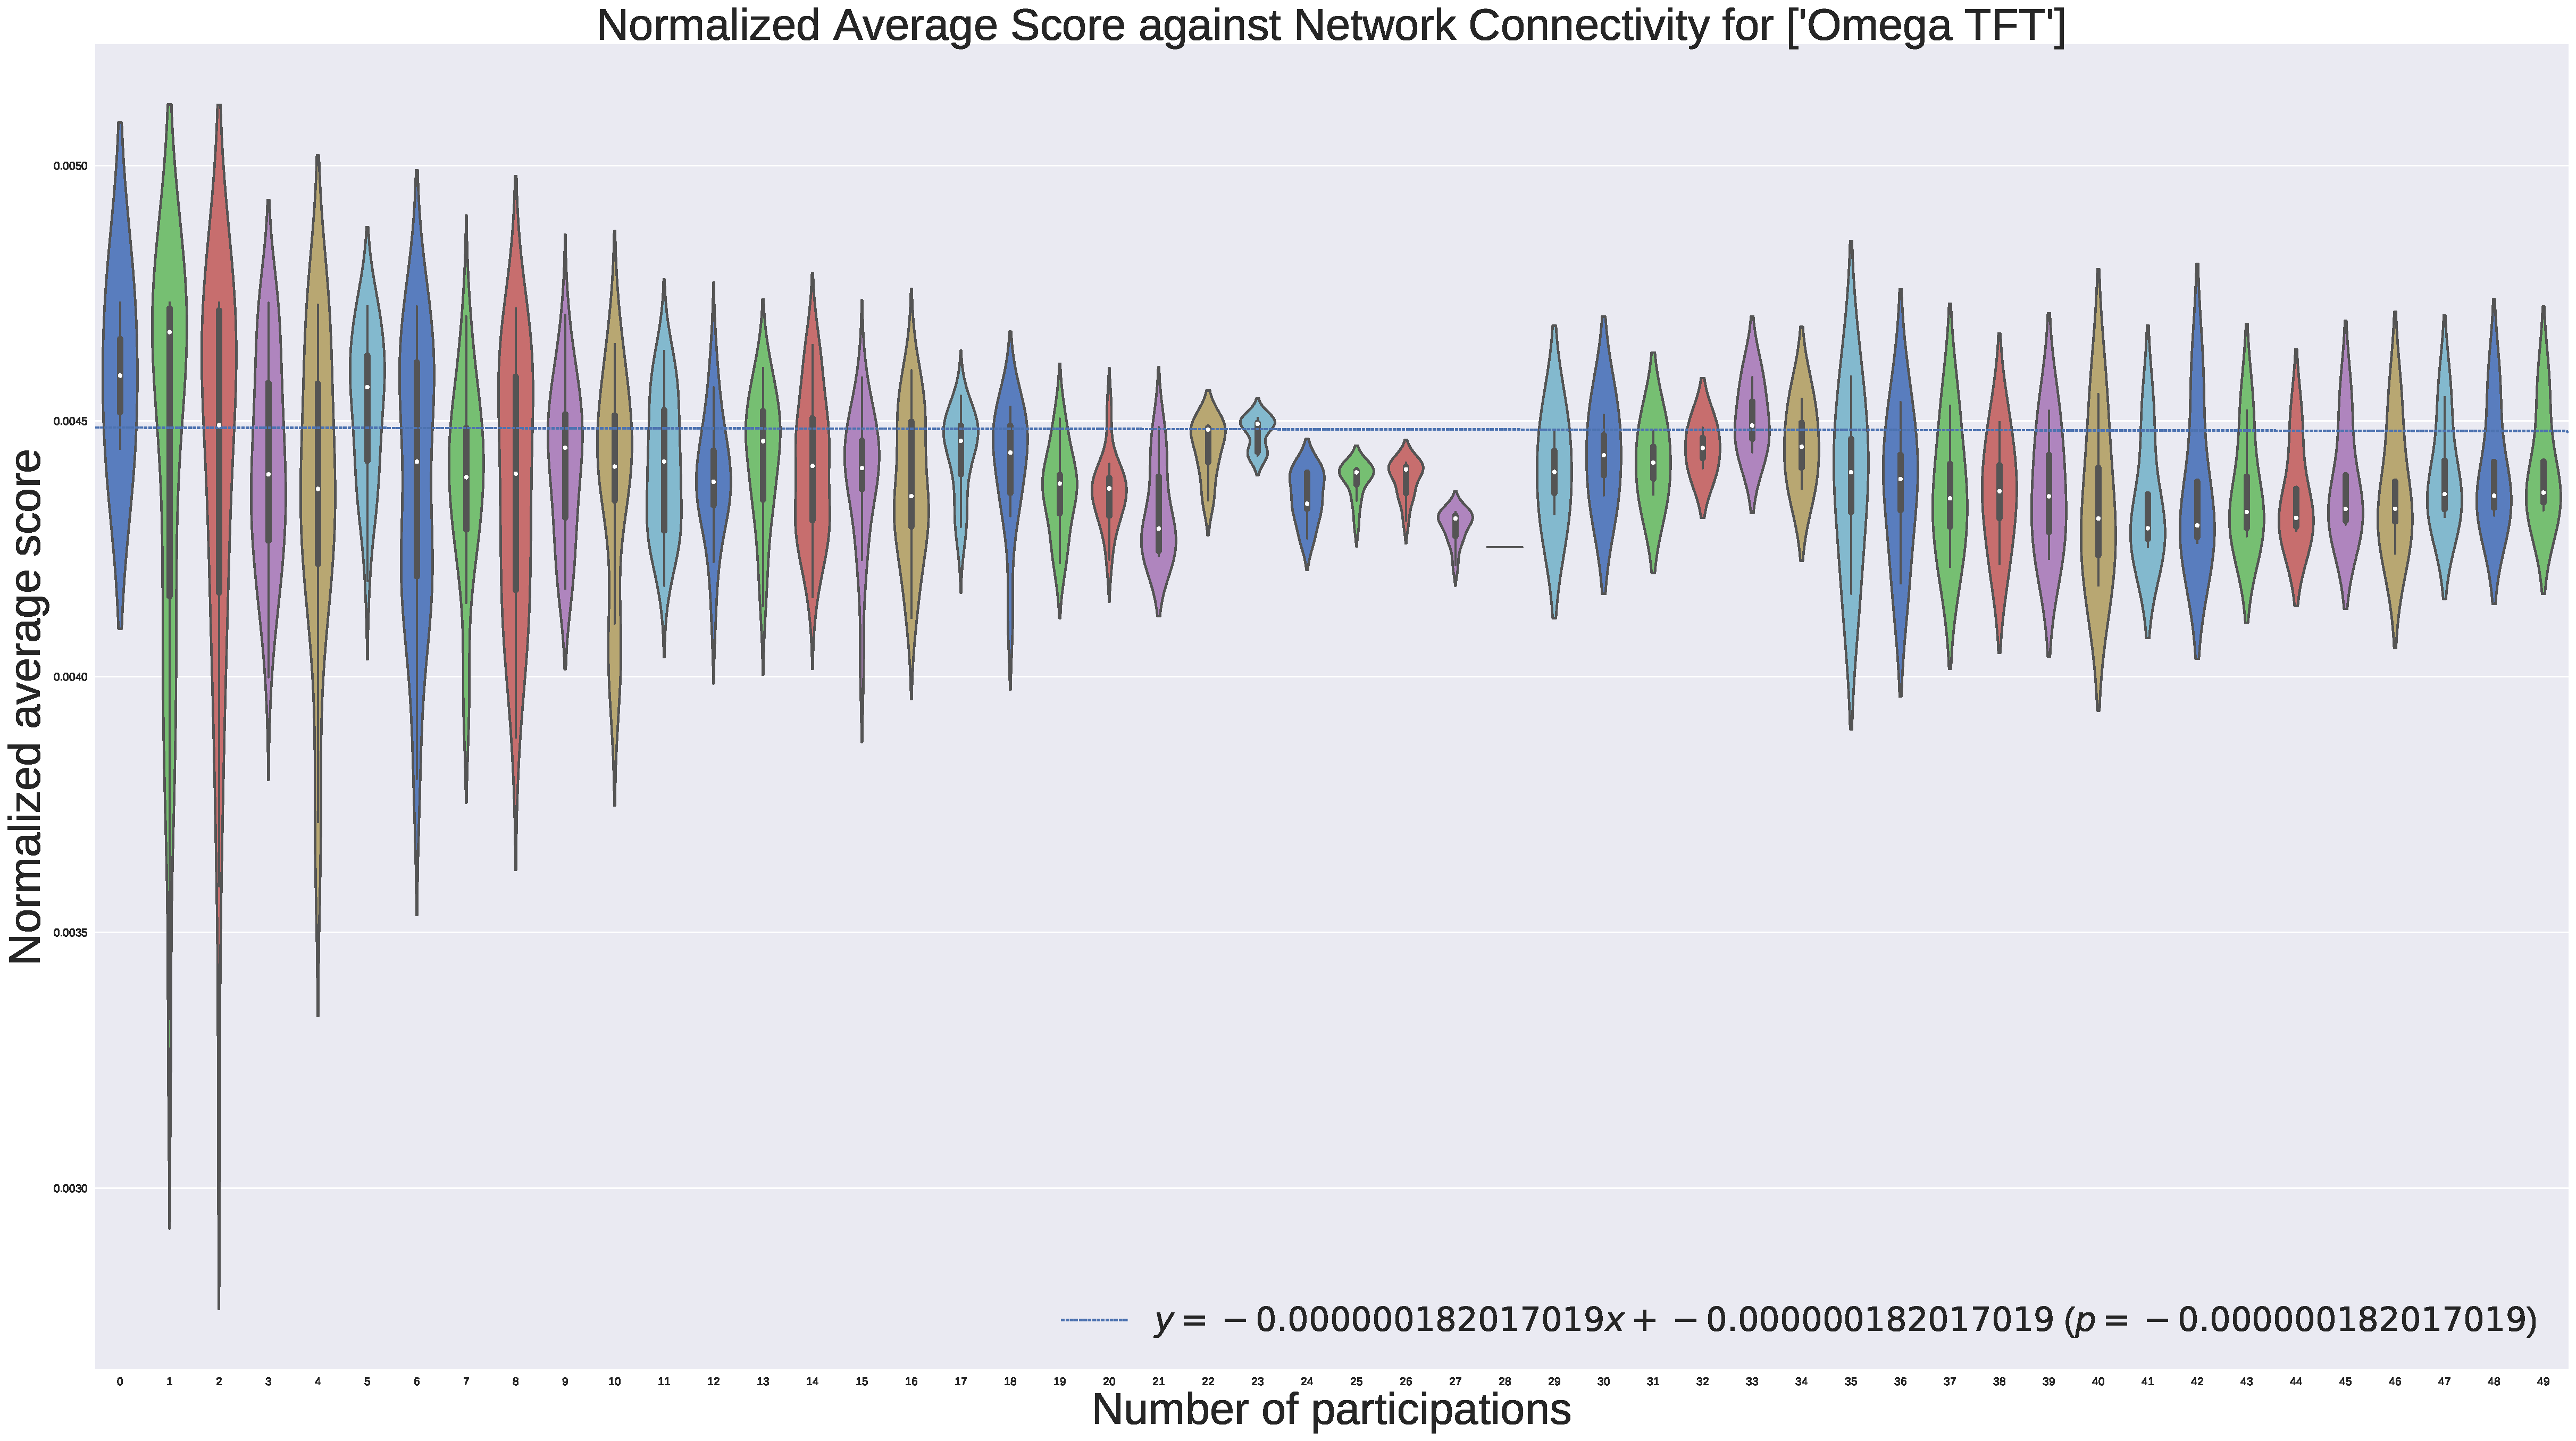
\includegraphics[width=\linewidth]{chapter-four/normalized-['OmegaTFT'].pdf}
		\caption{Normalized Average Score Omega TFT}
	\end{subfigure}
	\hfill
	\begin{subfigure}[t]{0.70\textwidth}\centering
		\centering
		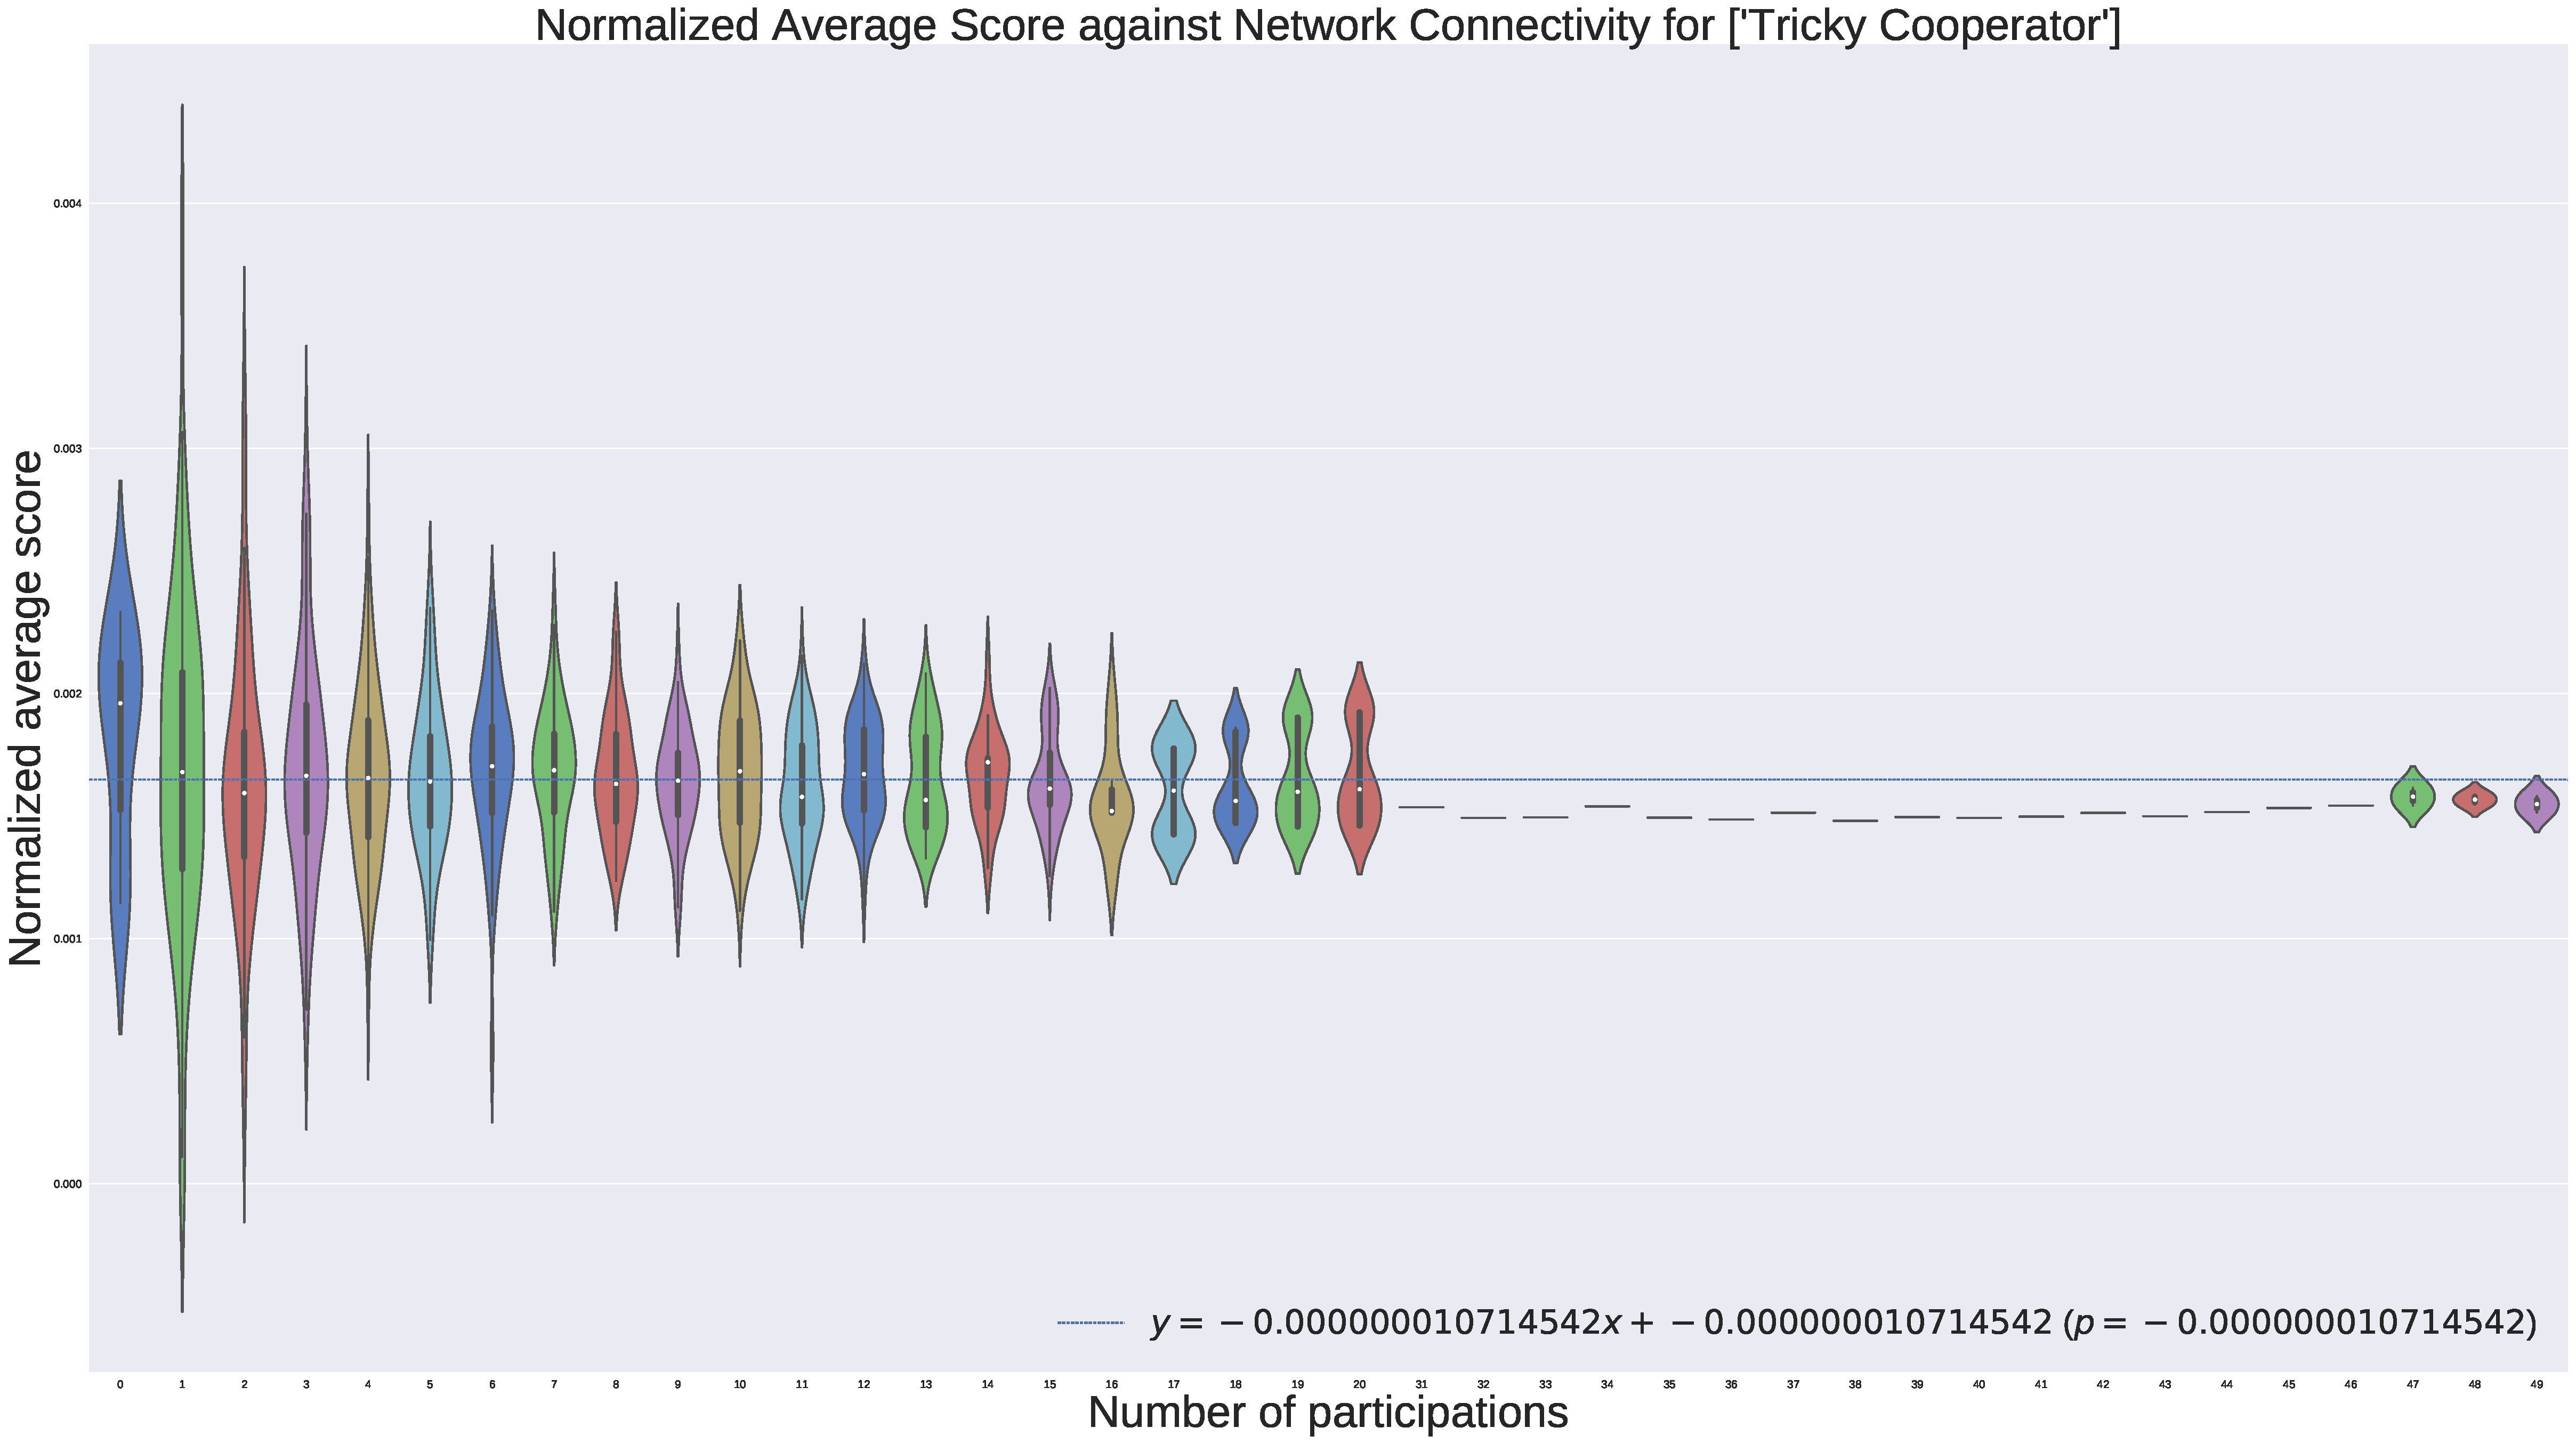
\includegraphics[width=\linewidth]{chapter-four/normalized-['TrickyCooperator'].pdf}
		\caption{Normalized Average Score Tricky Cooperator}
	\end{subfigure}
	\caption{Normalized Average Score}
	\label{normalized-av-scr}
\end{figure}

The fact that numerous, Kruskal Wallis tests return that there was no significant
difference between groups could indicate, that some strategies where not affected
by the topology, thus could have performed well in any given topology.
To further investigate this, a more appropriate measure of performance is
introduced in the following subsection. Where more Kruskal wallis tests and
other statistical analysis has been held.

\subsection{Normalized Median Rank}

This part of the chapter, focuses on a new measure of performance. The
normalized median rank of the strategies. To compute the normalized median rank,
the rank for each strategy, for each participation is, divided by the corresponding
size of tournament. The median rank is believe to be a more accurate measure,
compared to the winning ratio. It will reveal strategies, that did not necessarily
achieved the maximum wins, but had an overall satisfying and smoothly
performance throughout the experiments.

By once again, concreting the data set by each strategy and computing the median
of the normalized ranks of each strategy, a point plot can have been created.
As illustrated in Figure~\ref{ranking-second-gen}.~\footnote{A reminder,the
	lowest the rank the higher a strategy scored. 0 is the highest rank a strategy
can achieve in a tournament.}
The strategies with the worst ranking are Meta Majority Finite Memory, Meta
Minority and Limited Retaliate (0.1/20). On the other hand, the highest ranked
strategies are the following:

\begin{itemize}
	\item Third with a median ranking equal to 0.27, Nydegger
	\item Second with a median ranking equal to 0.25, Cautious QLearner
	\item First with a median ranking equal to 0.23, Gradual
\end{itemize}

Nydegger, is a strategy which begins by playing  tit for tat for the first
three moves. Except if it was the only one to cooperate on the first move and
the only one to defect on the second move, it defects on the third move.
After the third move,  its choice is determined from the 3 preceding outcomes.
More detail information about the 3 preceding outcomes can be found in Appendix[].

Cautious QLearner, is a strategy that learns the best strategies through the
q-learning algorithm. Lastly Gradual, is a player that punishes defections with
a growing number of defections but after punishing enters a calming state and
cooperates no matter what the opponent does for two rounds. All three strategies
are categorized as high cooperators and Gradual is a well performed strategy
in the actual Axelrod tournament as well.

\begin{figure}[!hbtp]
	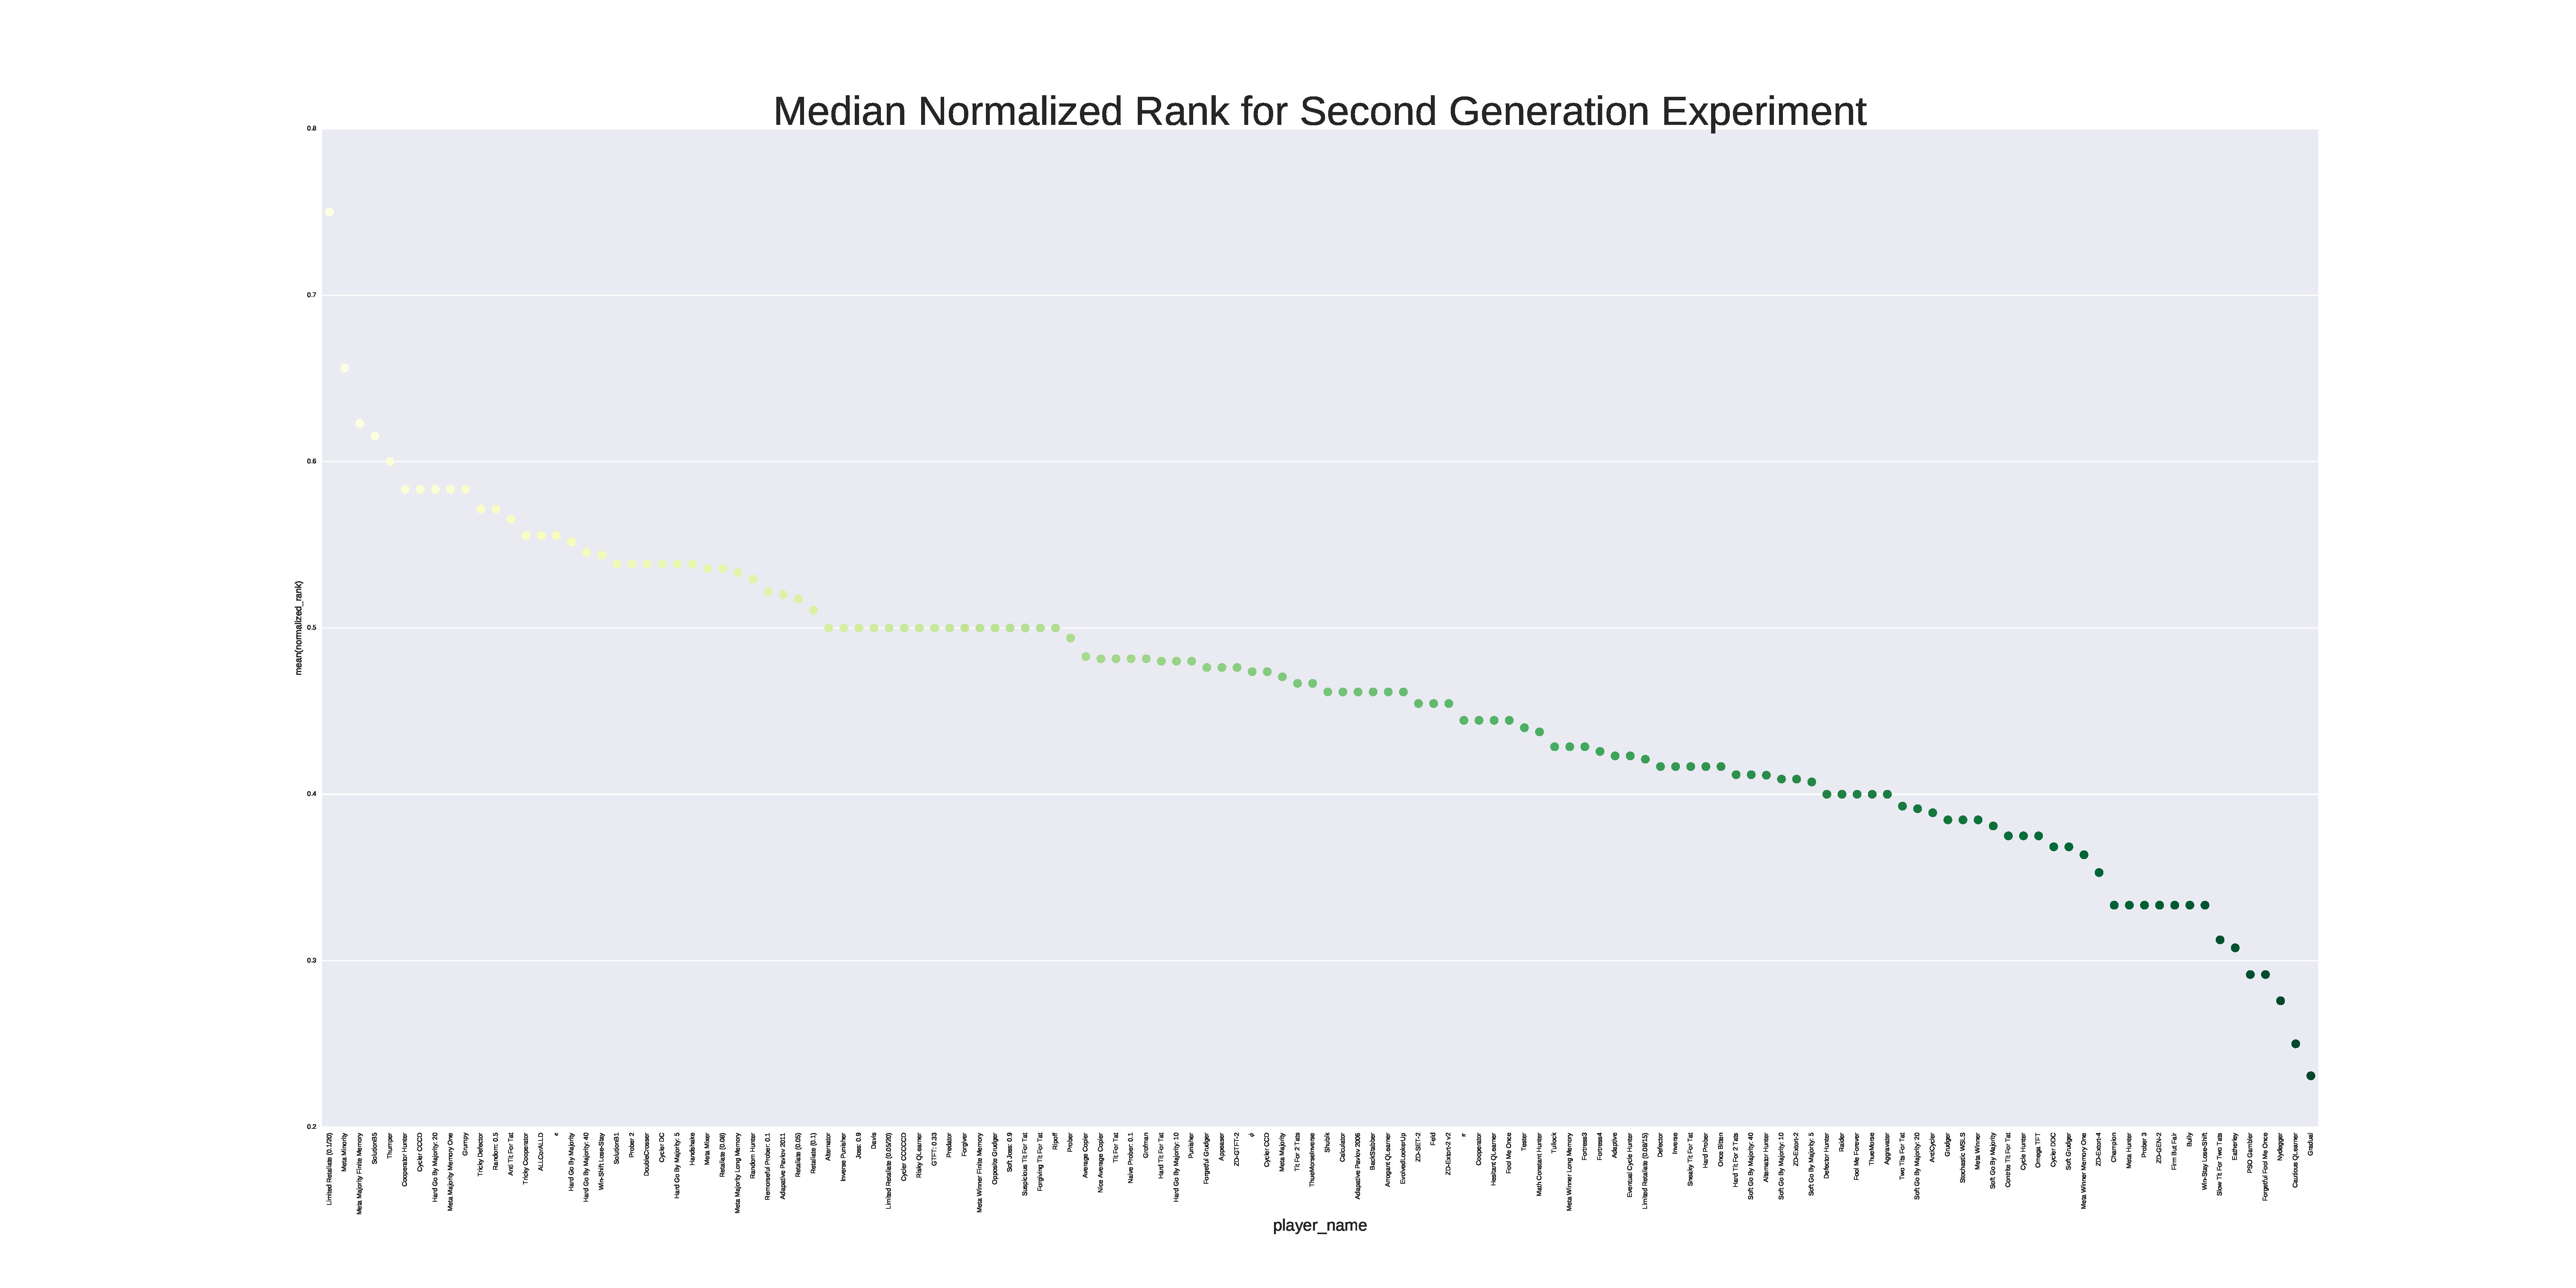
\includegraphics[width=1.2\linewidth,center]{chapter-four/median-ranking.pdf}
	\caption{Normalized Median Rank Complex Networks Experiments}
	\label{ranking-second-gen}
\end{figure}

For further research on these three strategies, a Kruskal Wallis test
has been performed for their normalized rankings. Whether there is a significant
difference on the rankings between groups of, networks connectivity, clustering
and cooperating ratio has been examined. A non parametric test is used, because
ranks are not a normally distributed measure.

For the clustering and cooperating ratio, a \(k\)-means algorithm has been used,
to create groups, 5 and 10 respectively. A table with the classification groups
can be found in the Appendix~\ref{append:class-top-strategies}.

The finding of the tests returned the following results. All \(p\) values, for
all three strategies, and all three
categories are lower that 0.05. Thus, there is significant difference between the
groups. The ranking of each three highest ranks strategies has been ranging, in
different topological environments. Violin plots for Cautious are shown
in Figure~\ref{cautious}, for in Nydegger in Figure~\ref{nydegger} and finally,
in Figure~\ref{gradual} Gradual.

\begin{figure}[!hbtp]
	\centering
	\begin{subfigure}[t]{0.70\textwidth}
		\centering
		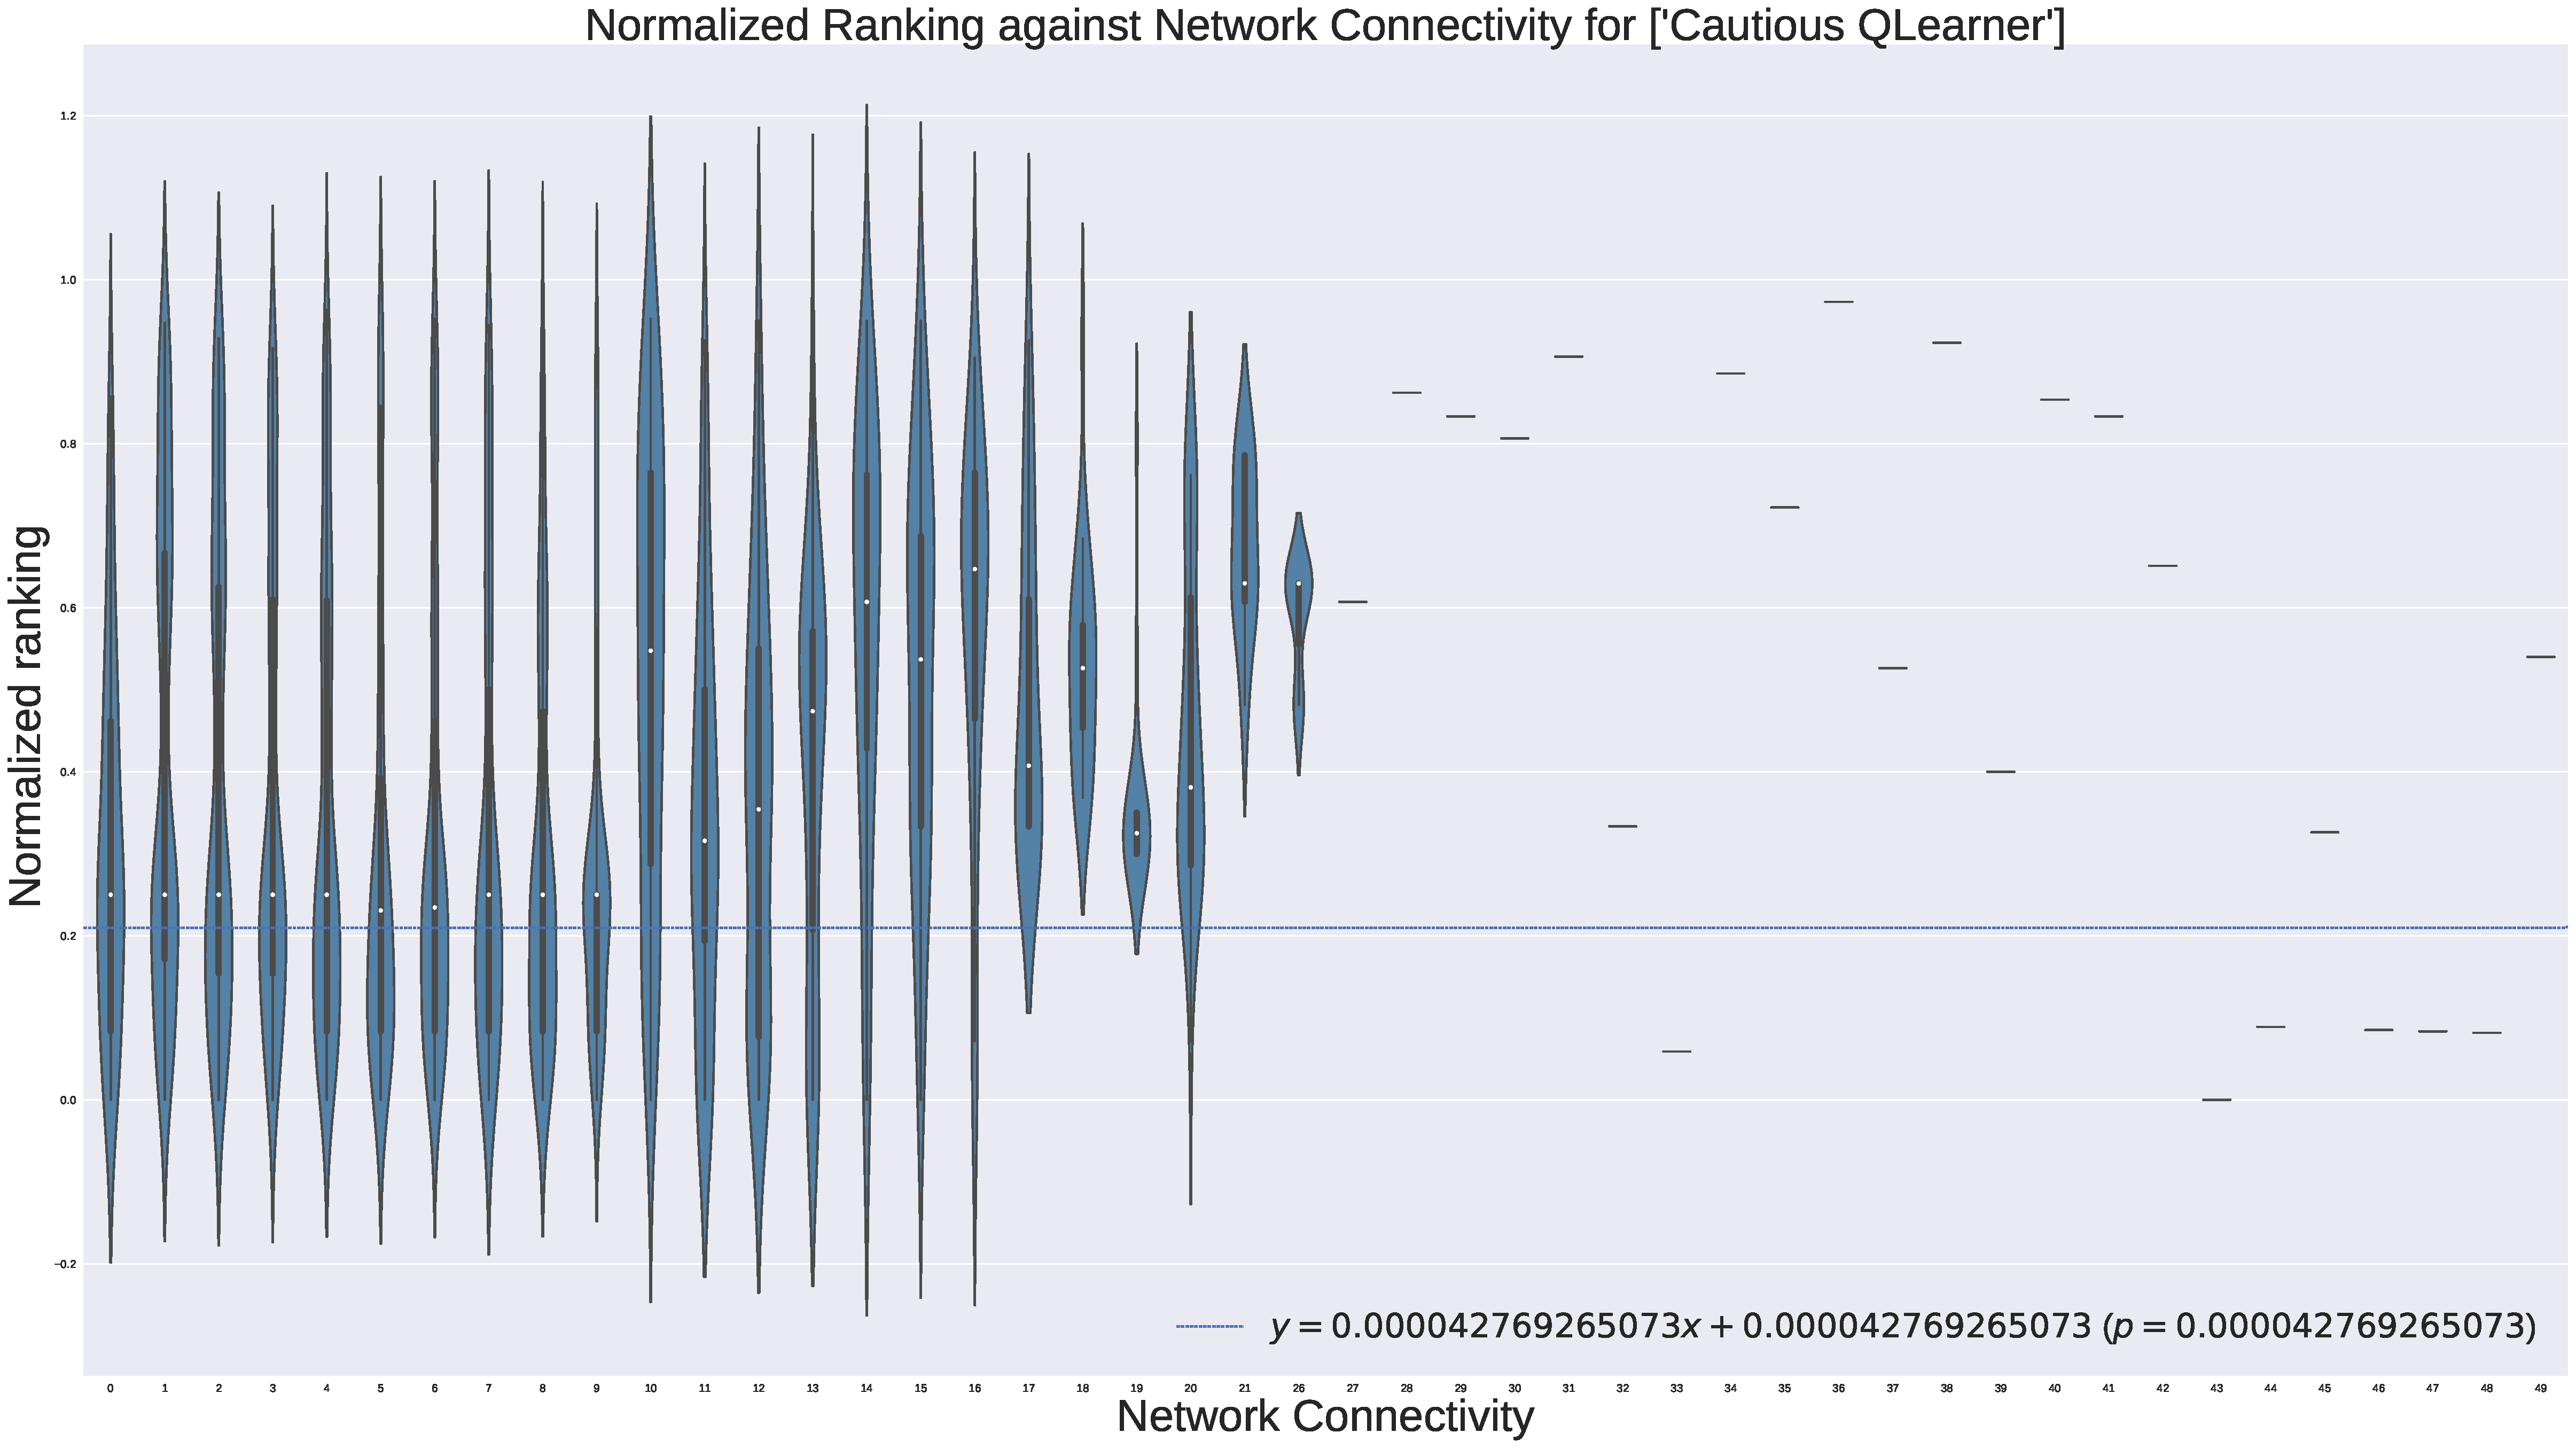
\includegraphics[width=\linewidth]{chapter-four/normalized-rank-['CautiousQLearner']-connectivity.pdf}
		\caption{Normalized Ranking against Network Connectivity}
	\end{subfigure}
	\hfill
	\begin{subfigure}[t]{0.70\textwidth}\centering
		\centering
		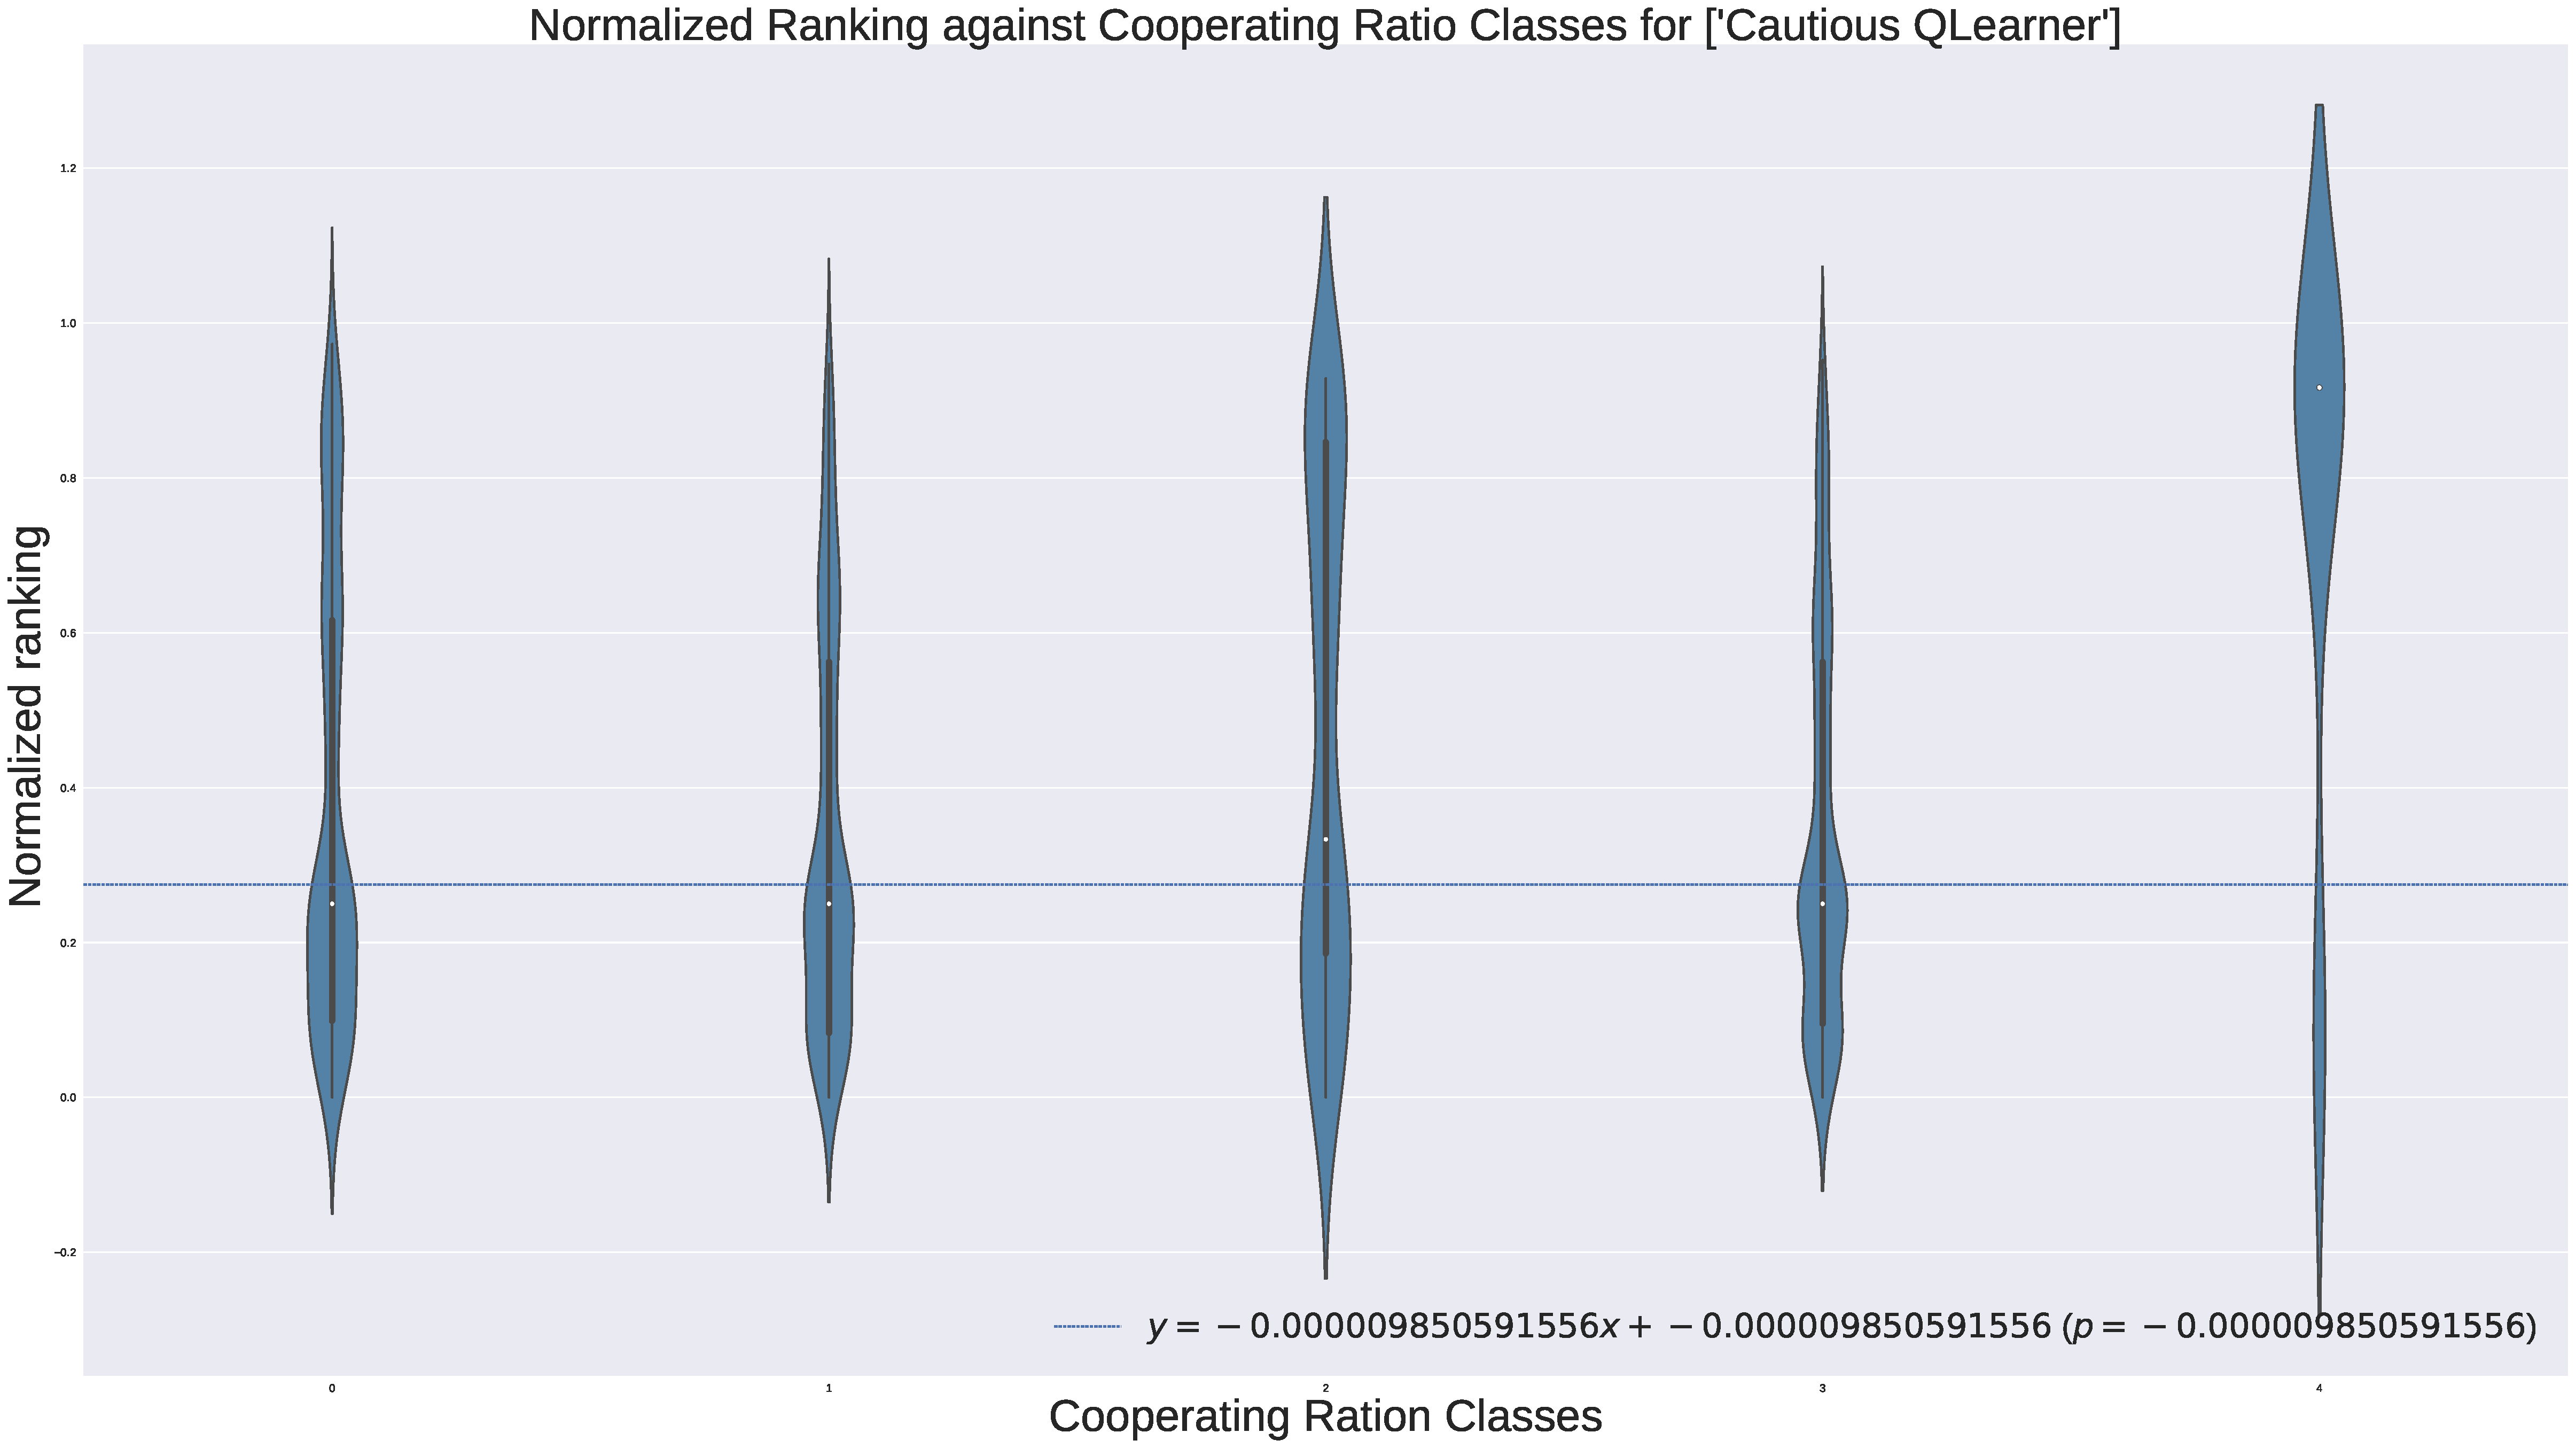
\includegraphics[width=\linewidth]{chapter-four/normalized-rank-['CautiousQLearner']-cooperating.pdf}
		\caption{Normalized Ranking against Cooperating Ratio Classes}
	\end{subfigure}
	\hfill
	\begin{subfigure}[t]{0.70\textwidth}\centering
		\centering
		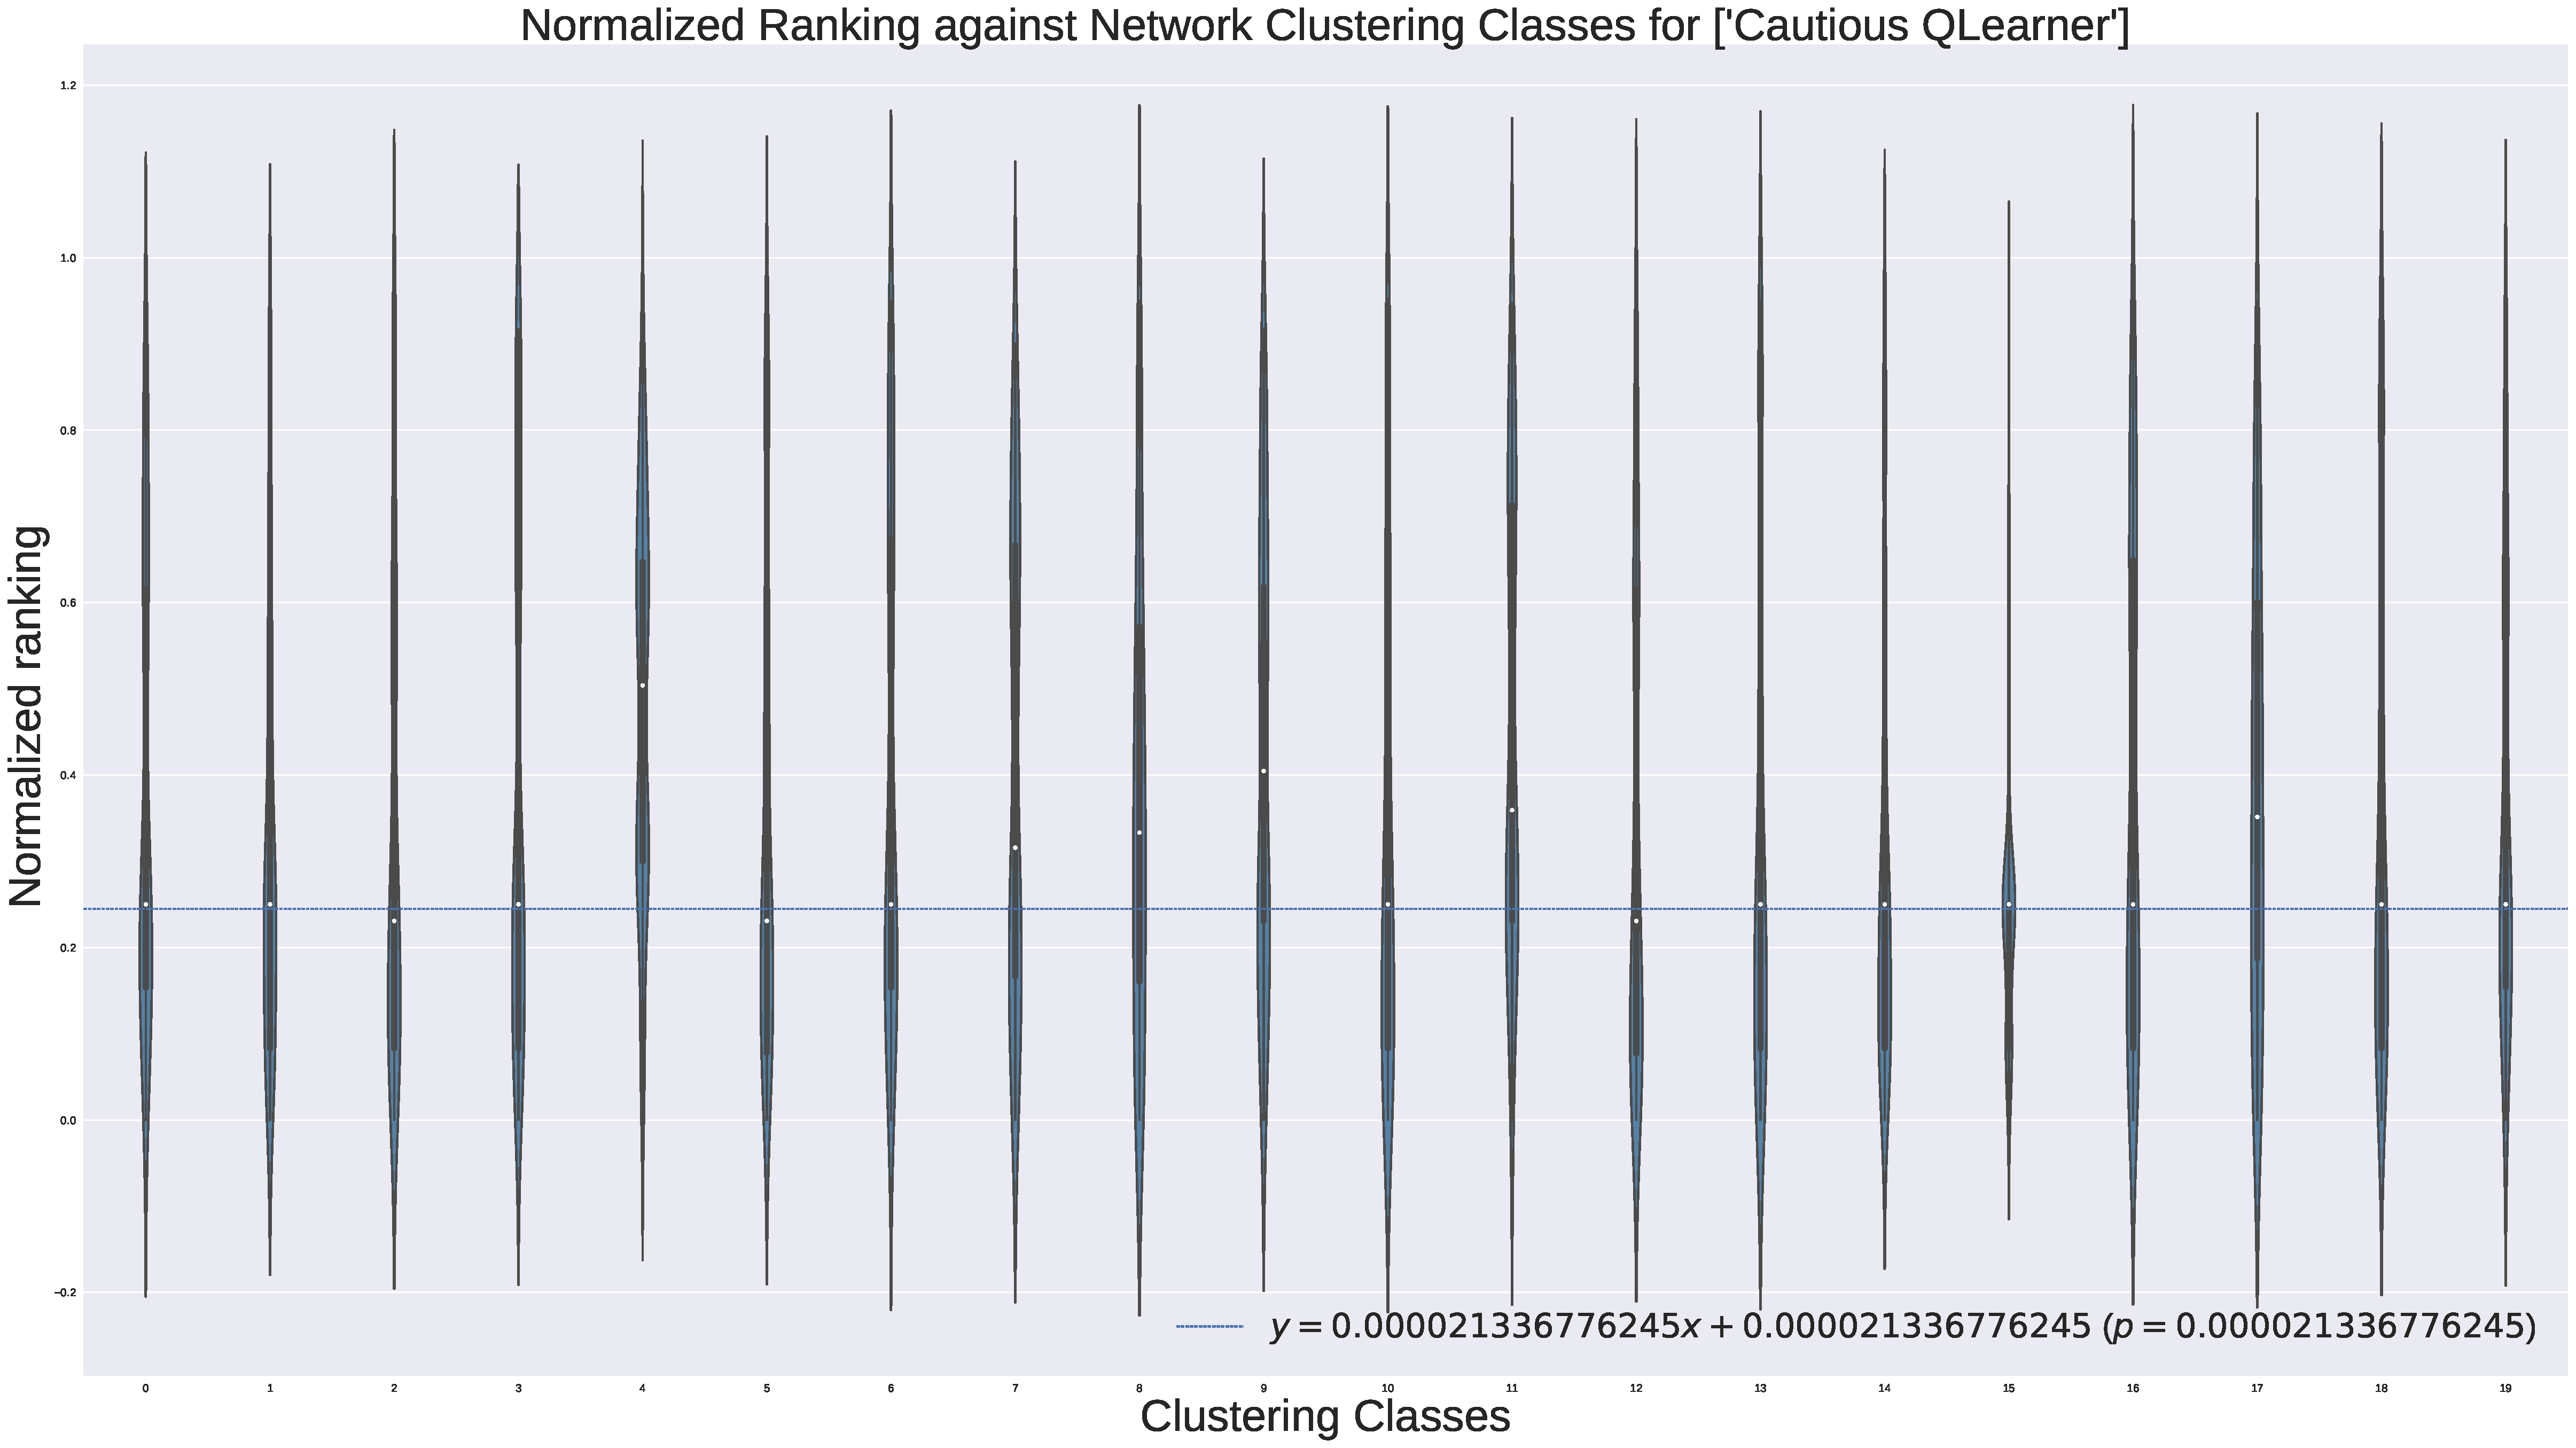
\includegraphics[width=\linewidth]{chapter-four/normalized-rank-['CautiousQLearner']-clustering.pdf}
		\caption{Normalized Ranking against Network Clustering Classes}
	\end{subfigure}
	\caption{Normalized Ranking Violin Plots for Cautious QLearner}
	\label{cautious}
\end{figure}

\begin{figure}[!hbtp]
	\centering
	\begin{subfigure}[t]{0.70\textwidth}
		\centering
		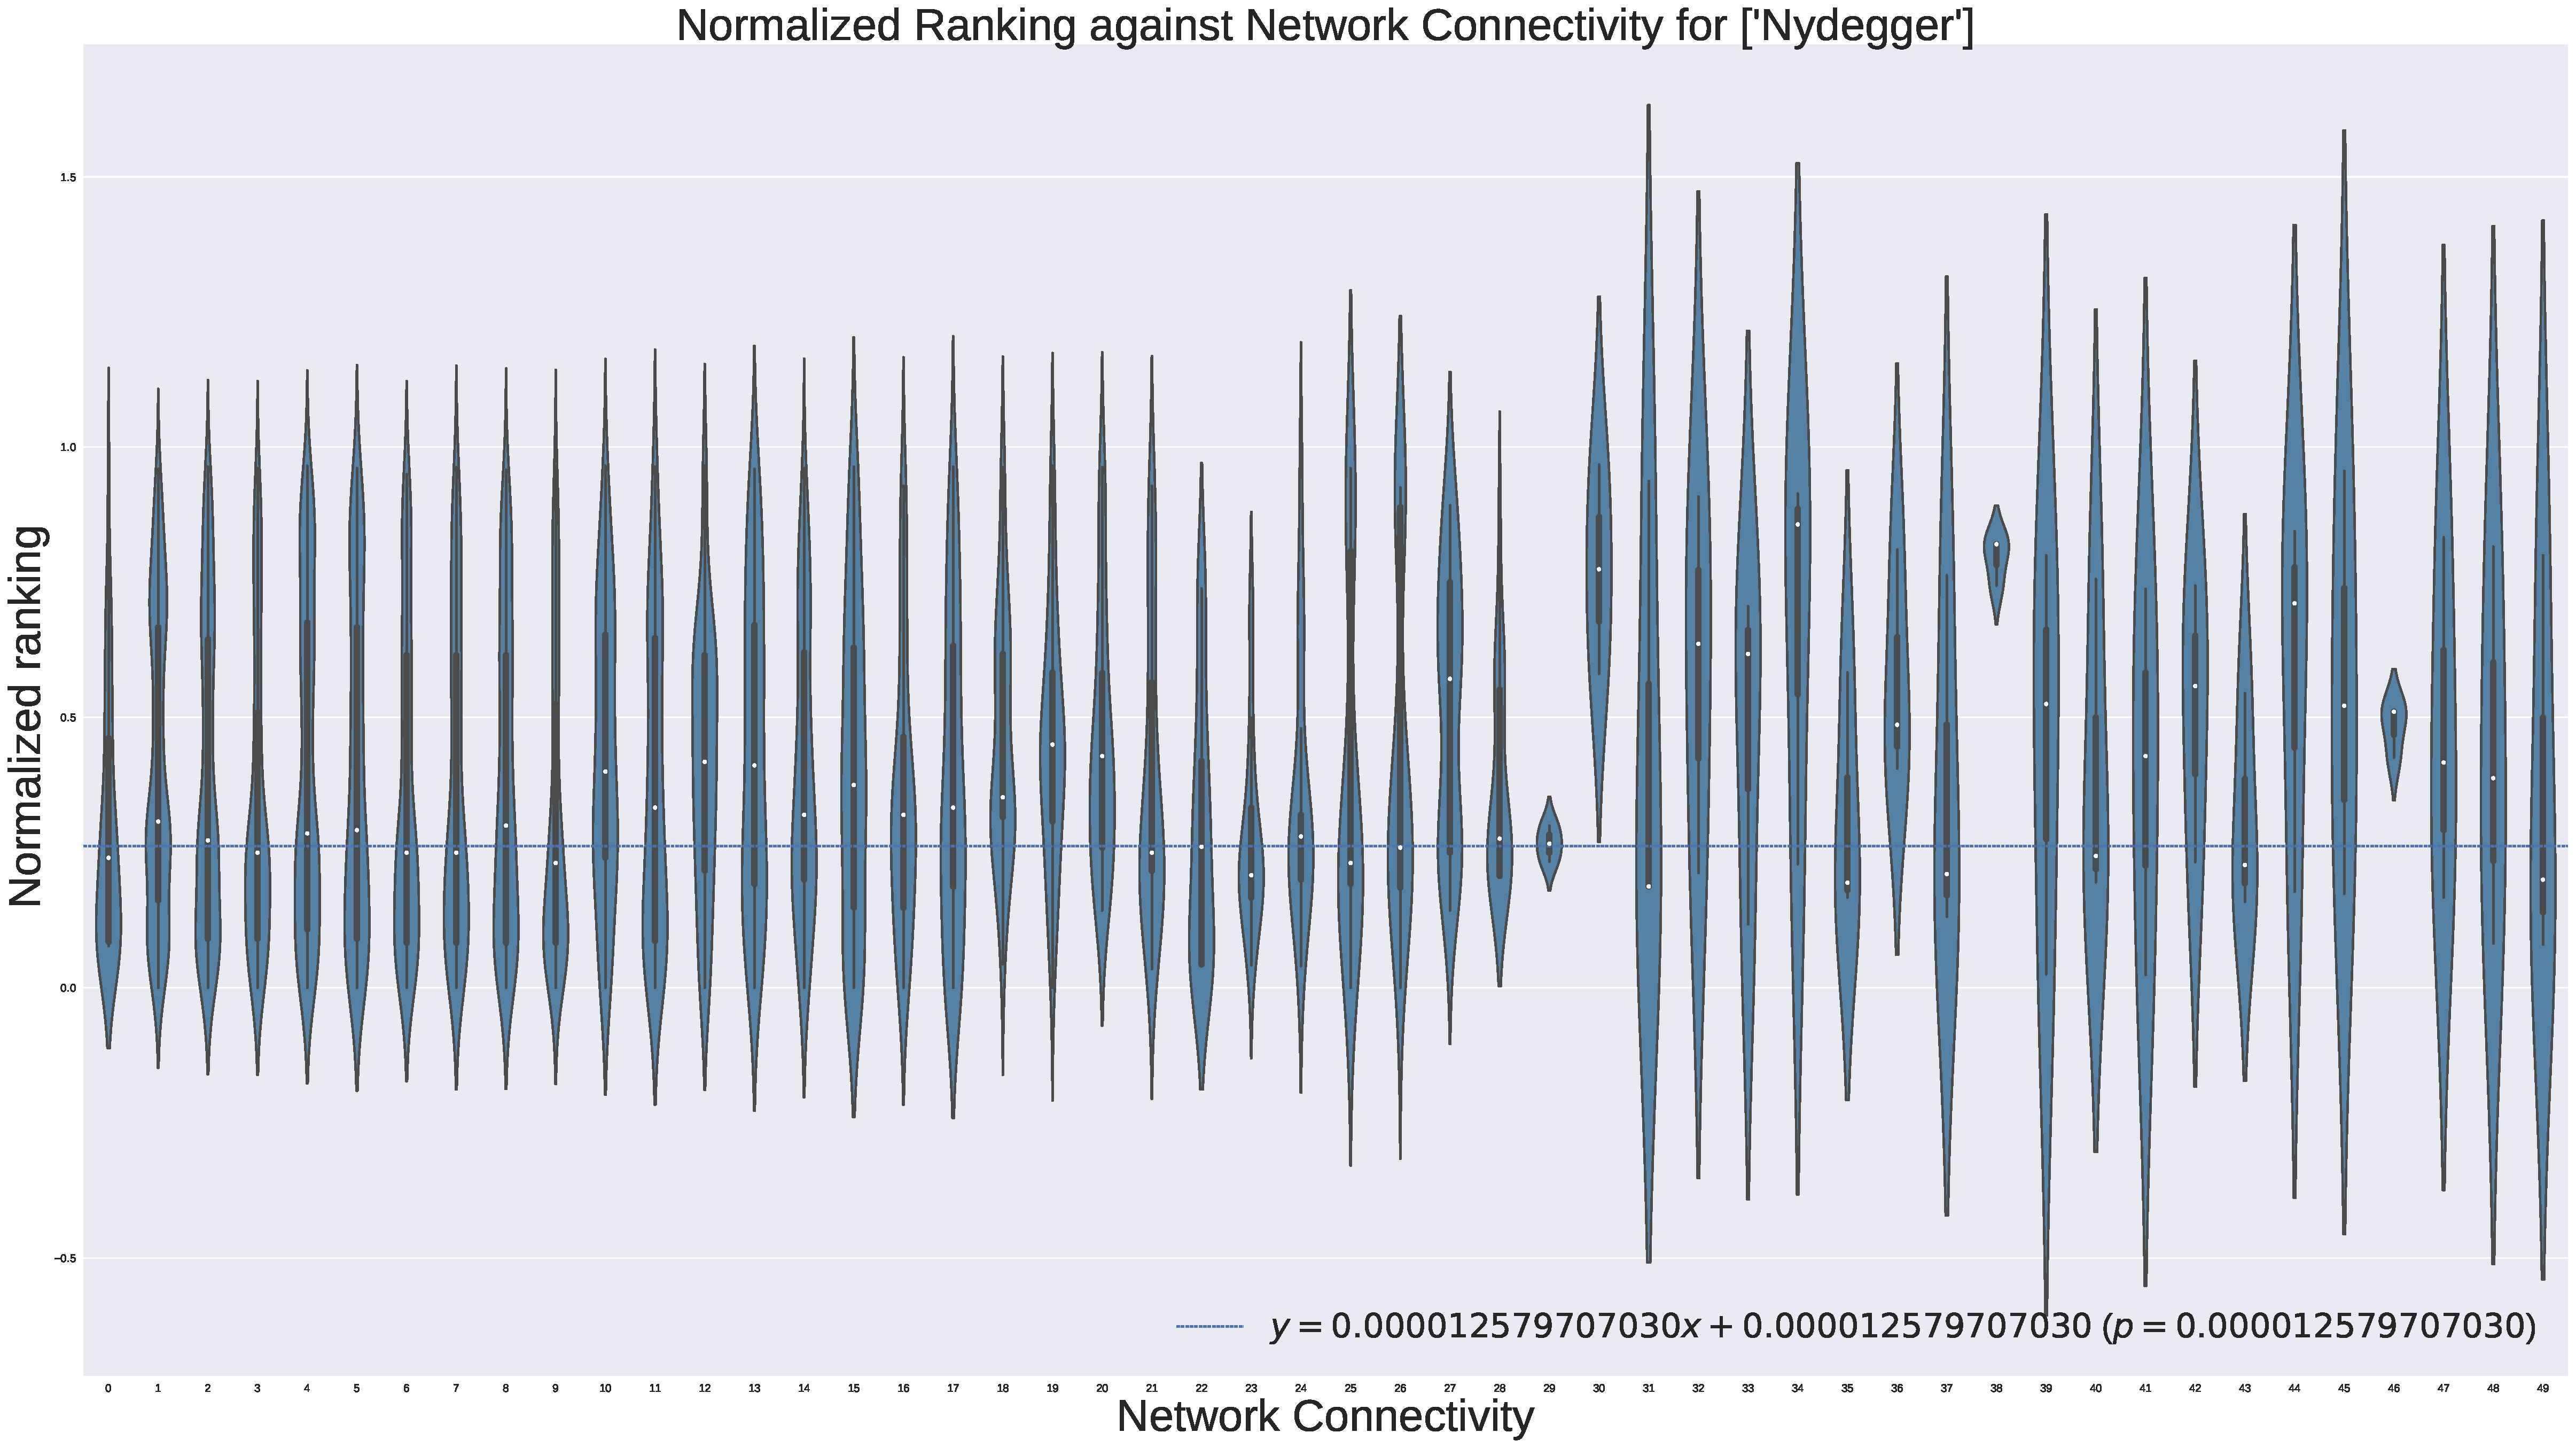
\includegraphics[width=\linewidth]{chapter-four/normalized-rank-['Nydegger']-connectivity.pdf}
		\caption{Normalized Ranking against Network Connectivity}
	\end{subfigure}
	\hfill
	\begin{subfigure}[t]{0.70\textwidth}\centering
		\centering
		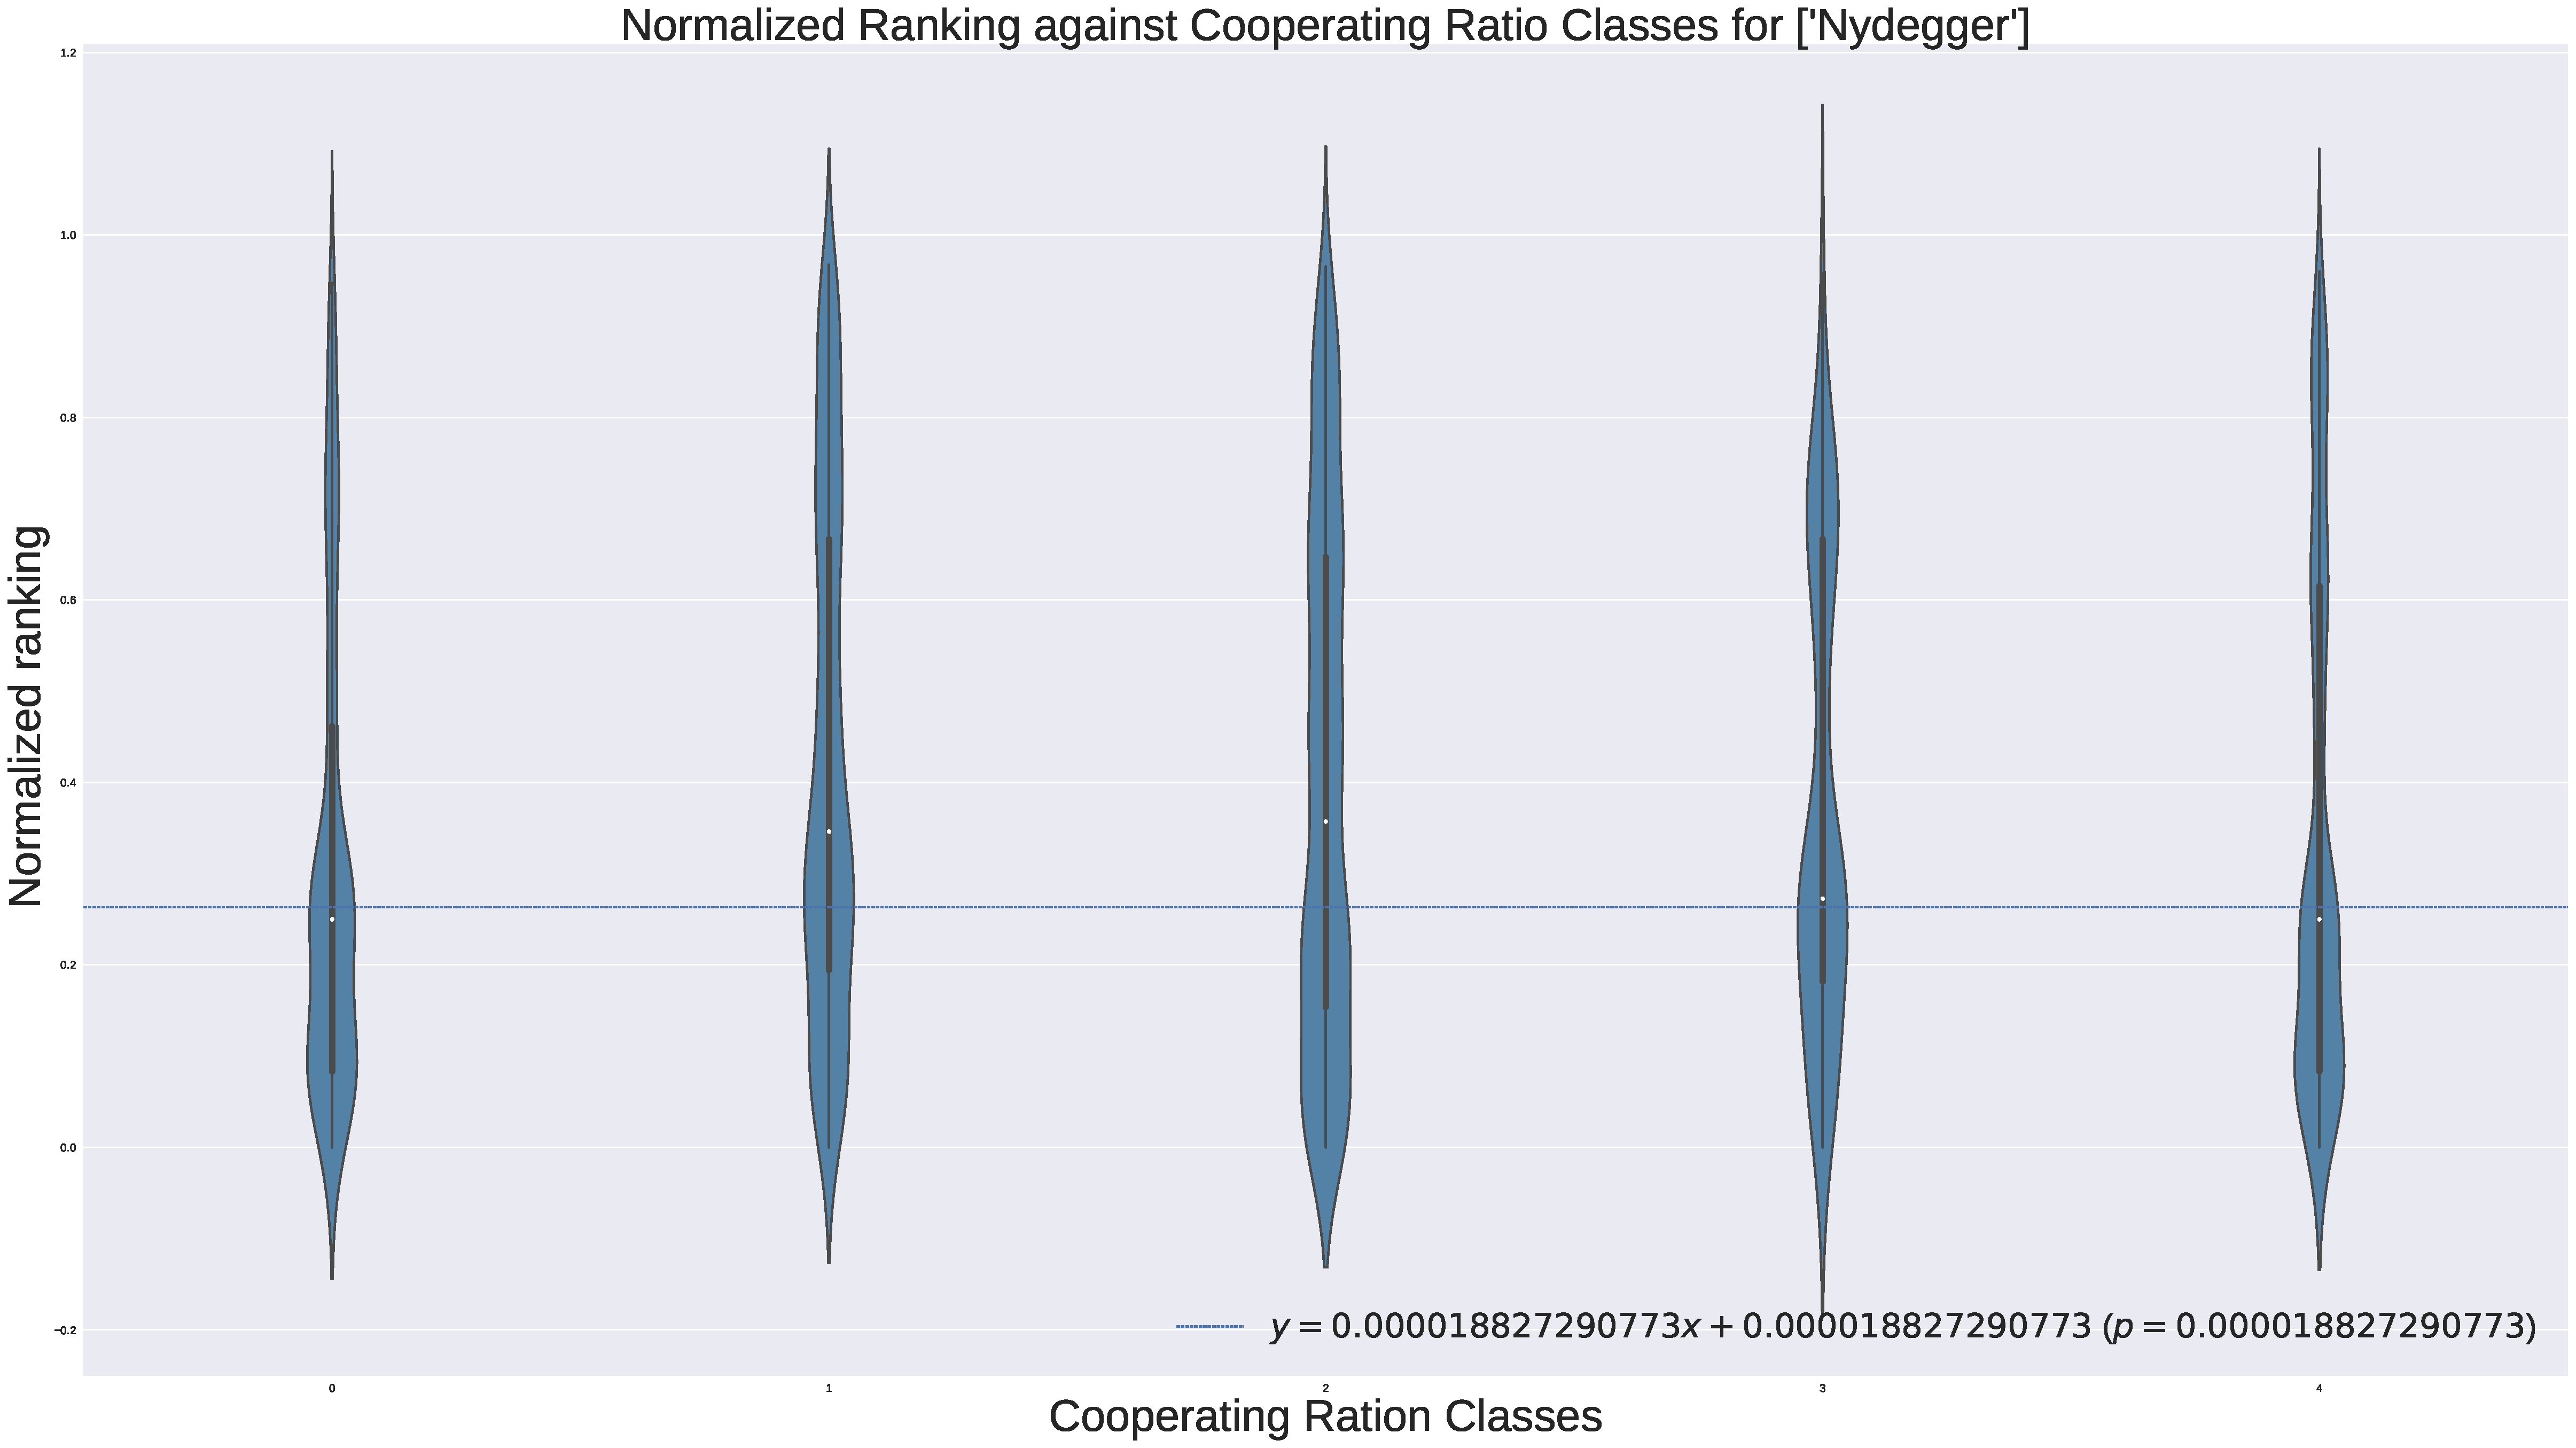
\includegraphics[width=\linewidth]{chapter-four/normalized-rank-['Nydegger']-cooperating.pdf}
		\caption{Normalized Ranking against Cooperating Ratio Classes}
	\end{subfigure}
	\hfill
	\begin{subfigure}[t]{0.70\textwidth}\centering
		\centering
		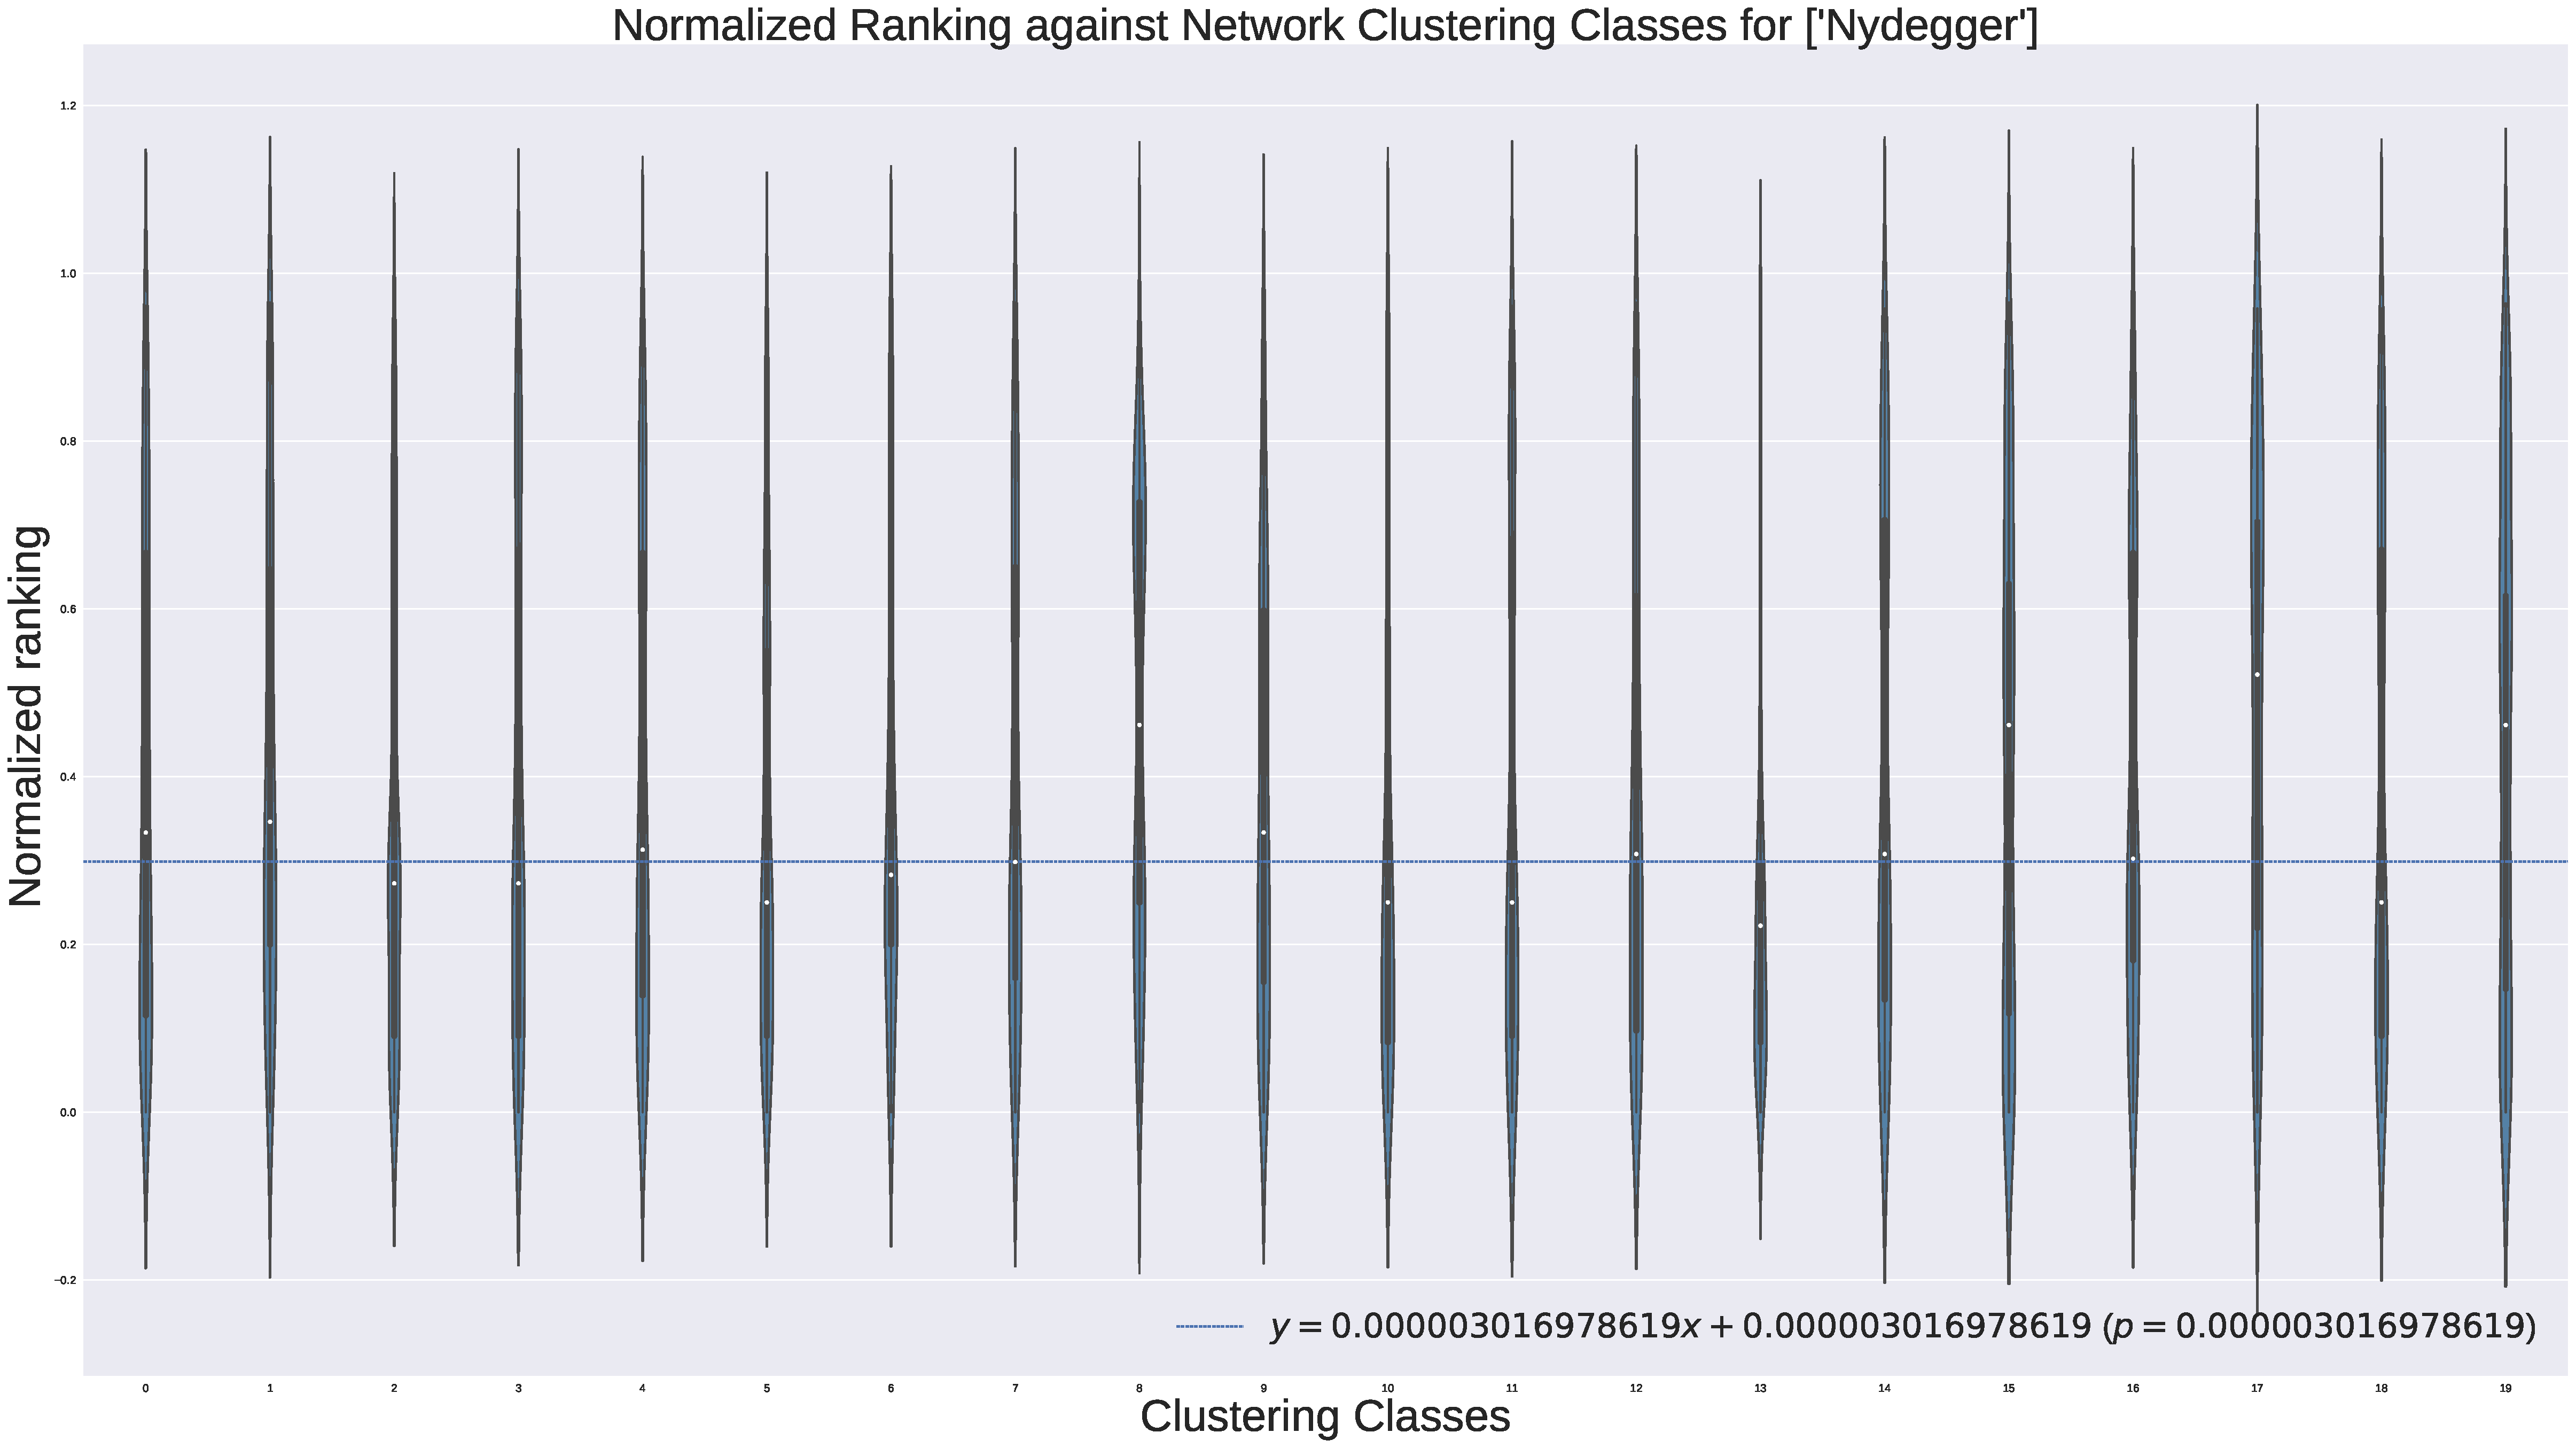
\includegraphics[width=\linewidth]{chapter-four/normalized-rank-['Nydegger']-clustering.pdf}
		\caption{Normalized Ranking against Network Clustering Classes}
	\end{subfigure}
	\caption{Normalized Ranking Violin Plots for Nydegger}
	\label{nydegger}
\end{figure}

\begin{figure}[!hbtp]
	\centering
	\begin{subfigure}[t]{0.70\textwidth}
		\centering
		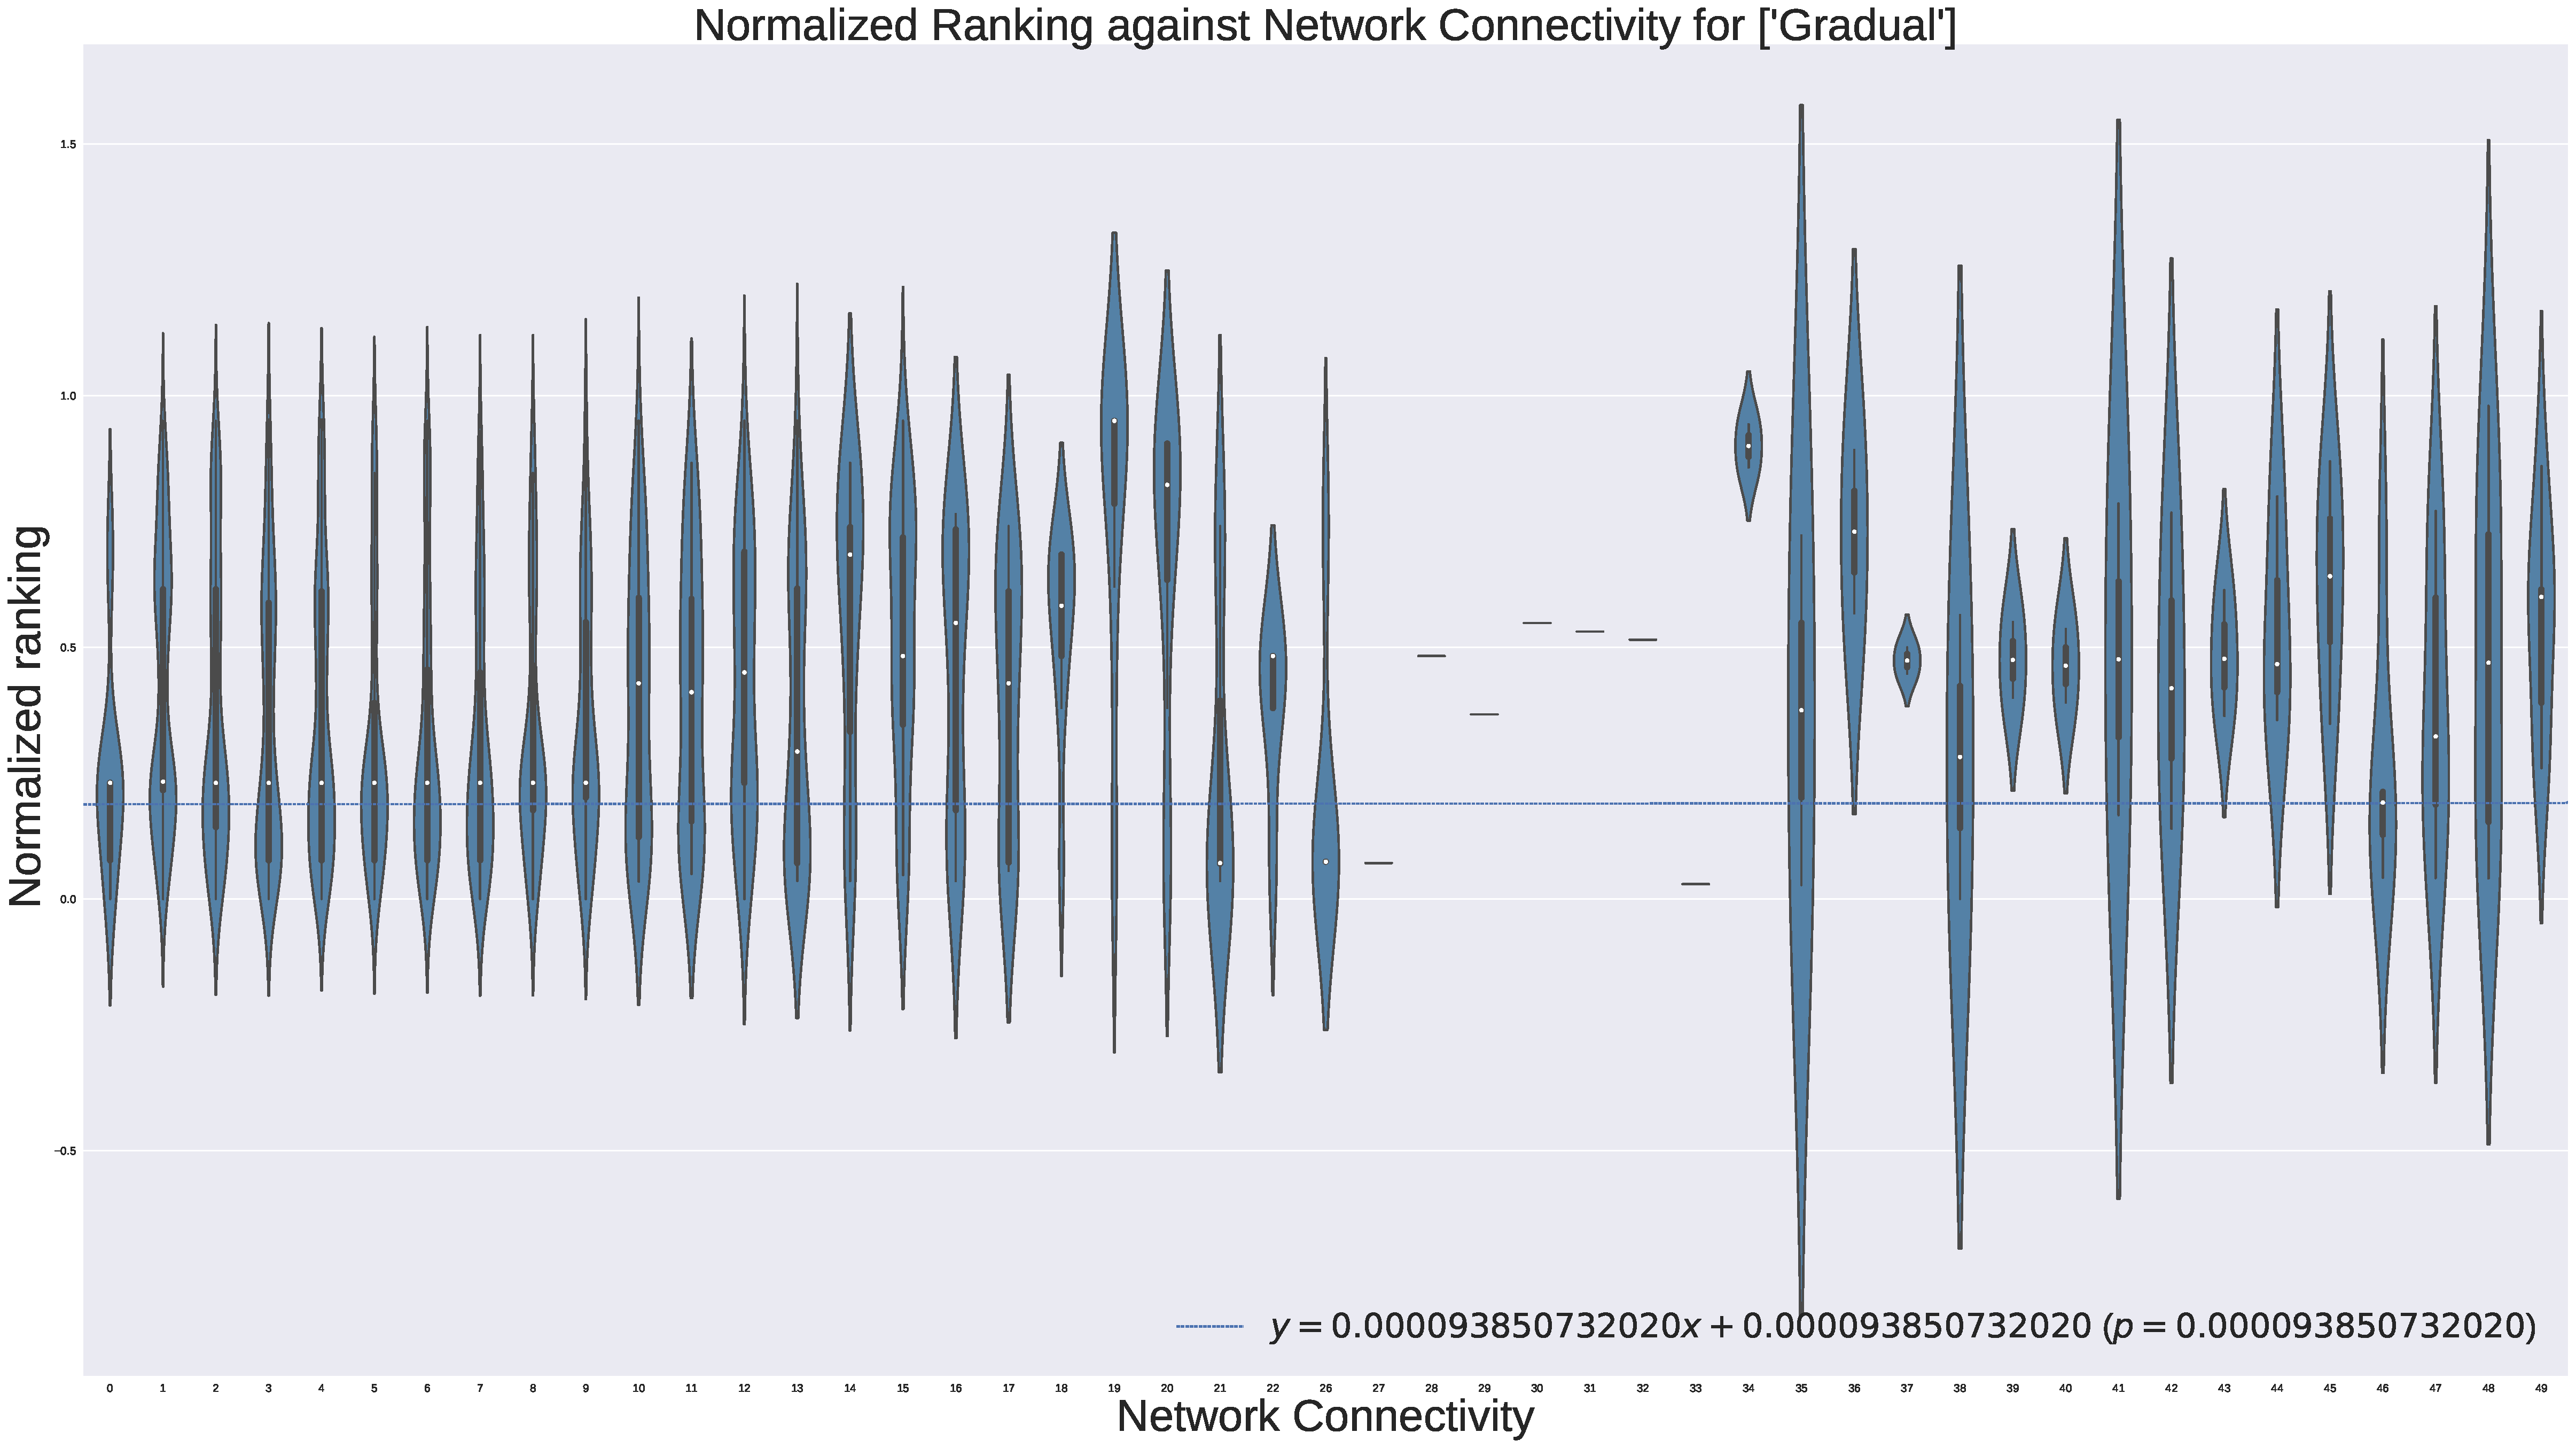
\includegraphics[width=\linewidth]{chapter-four/normalized-rank-['Gradual']-connectivity.pdf}
		\caption{Normalized Ranking against Network Connectivity}
	\end{subfigure}
	\hfill
	\begin{subfigure}[t]{0.70\textwidth}\centering
		\centering
		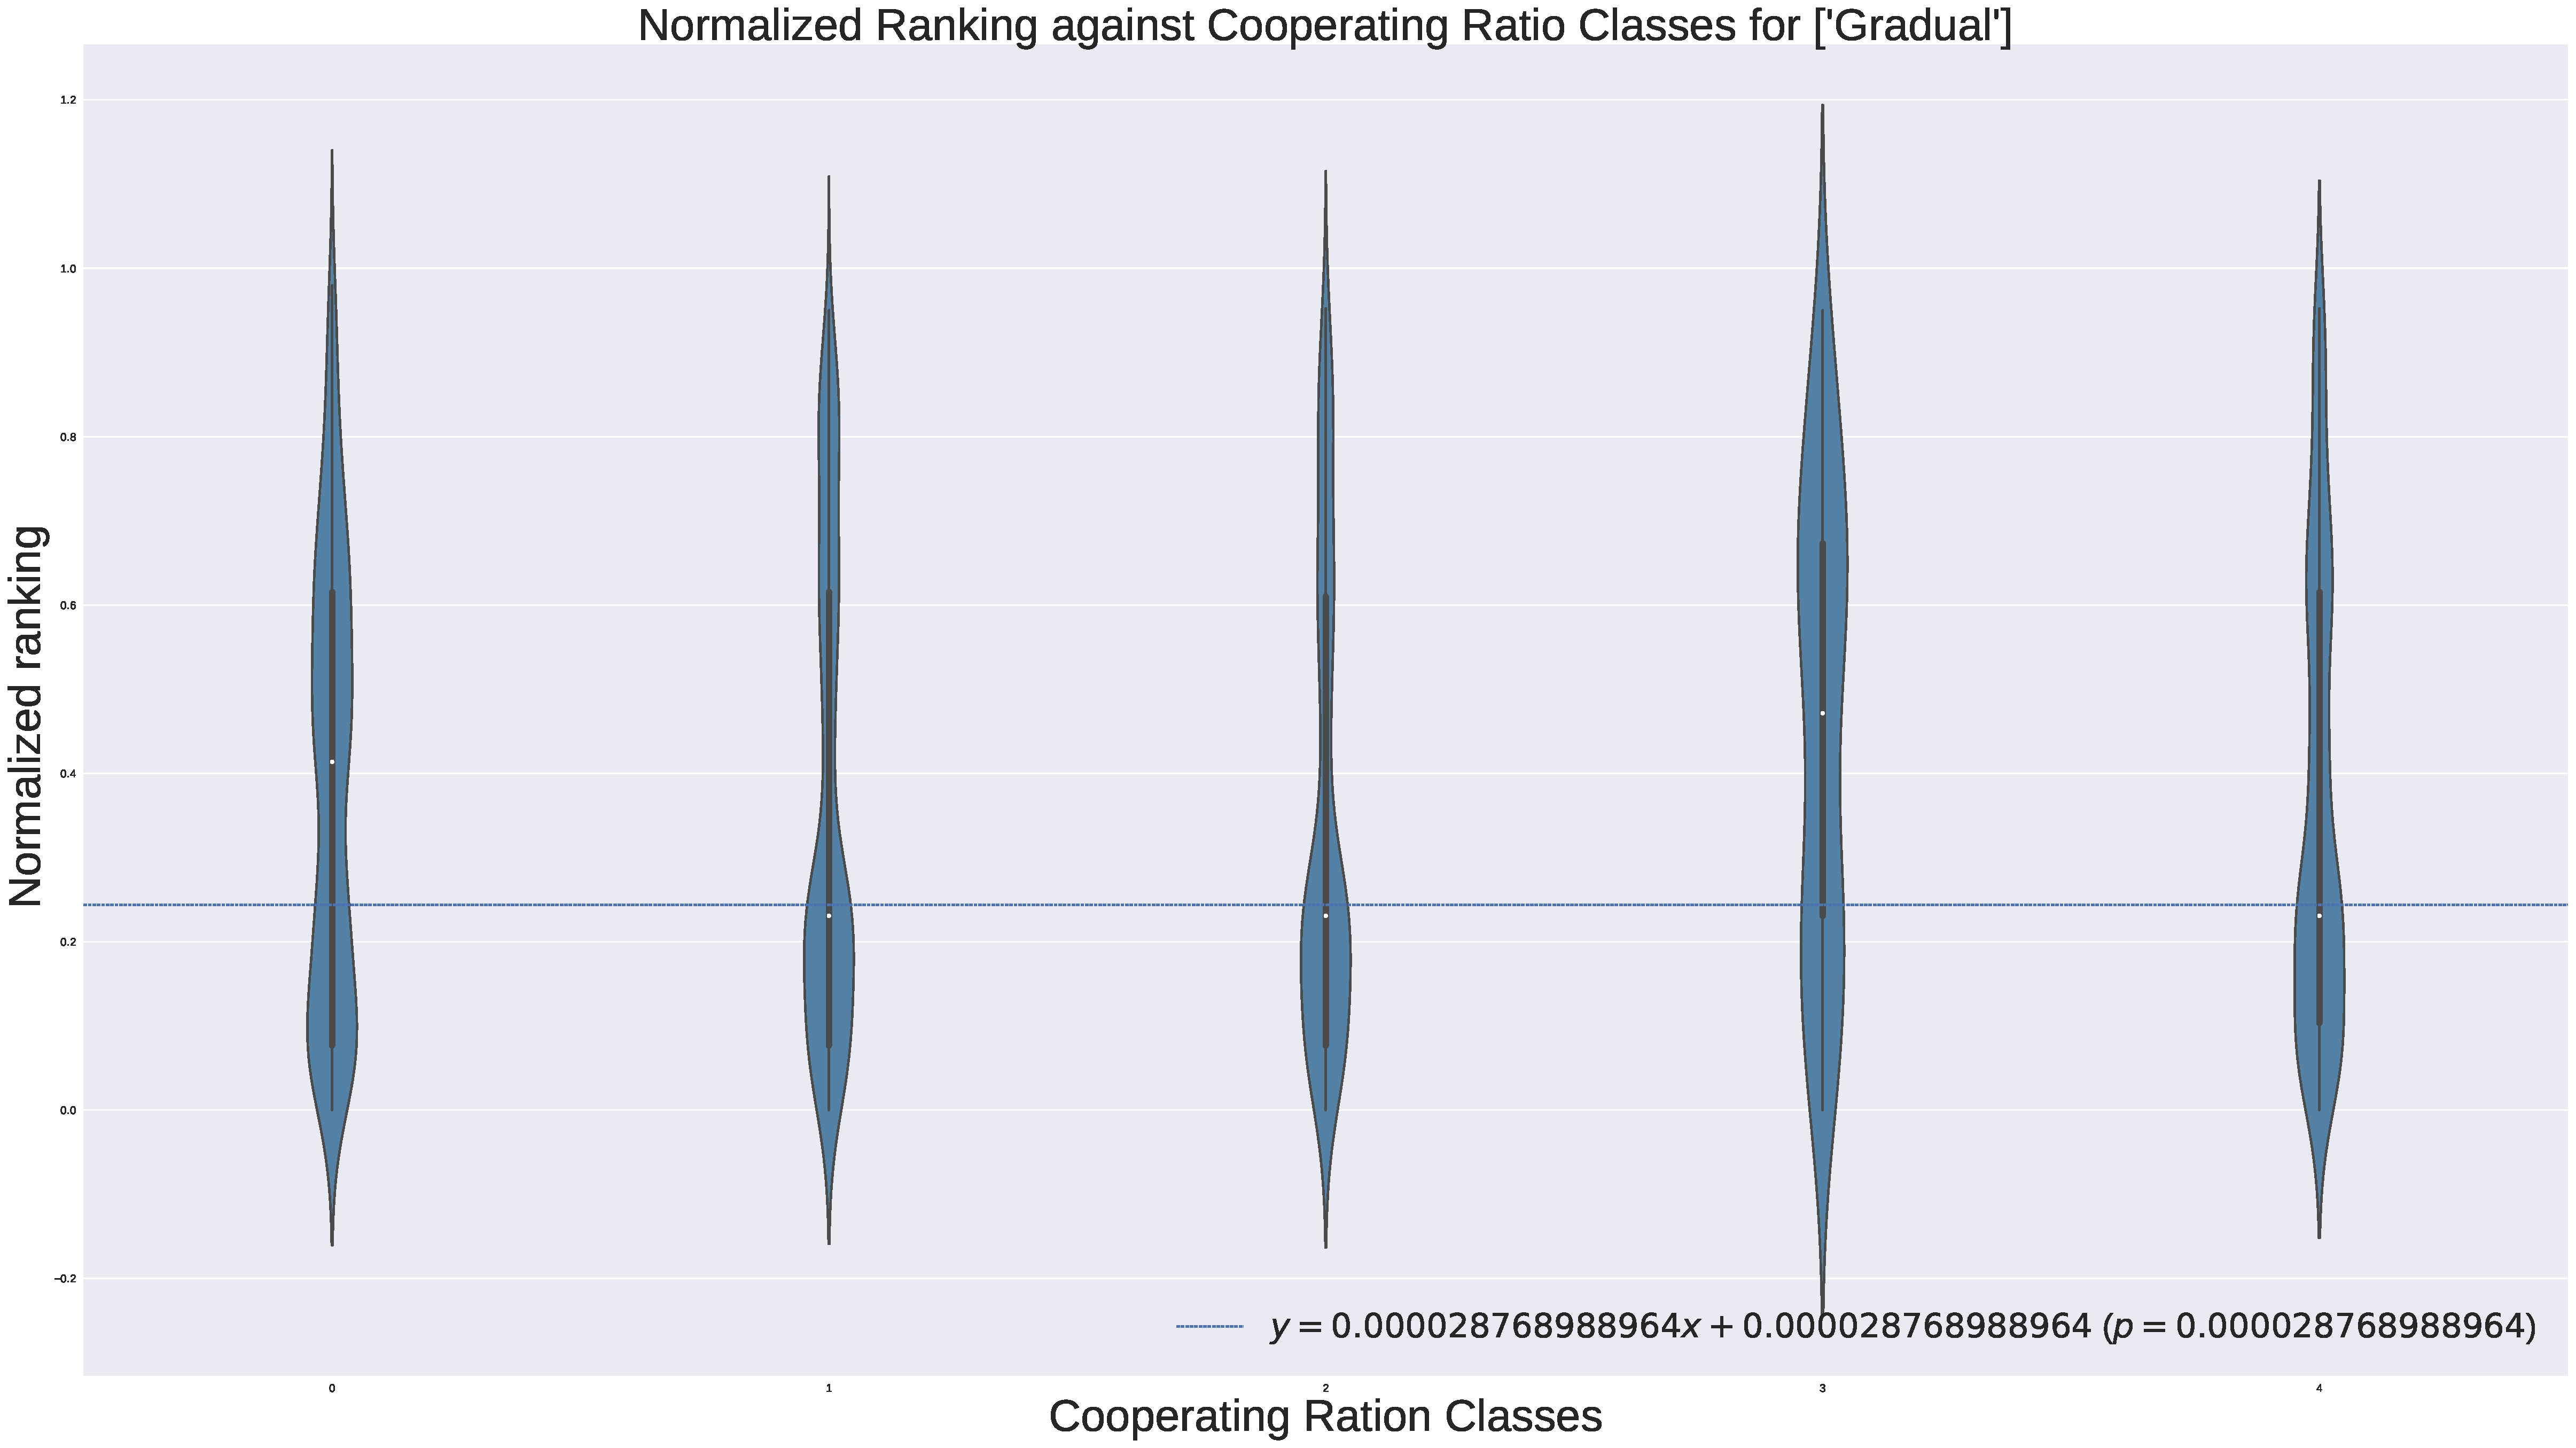
\includegraphics[width=\linewidth]{chapter-four/normalized-rank-['Gradual']-cooperating.pdf}
		\caption{Normalized Ranking against Cooperating Ratio Classes}
	\end{subfigure}
	\hfill
	\begin{subfigure}[t]{0.70\textwidth}\centering
		\centering
		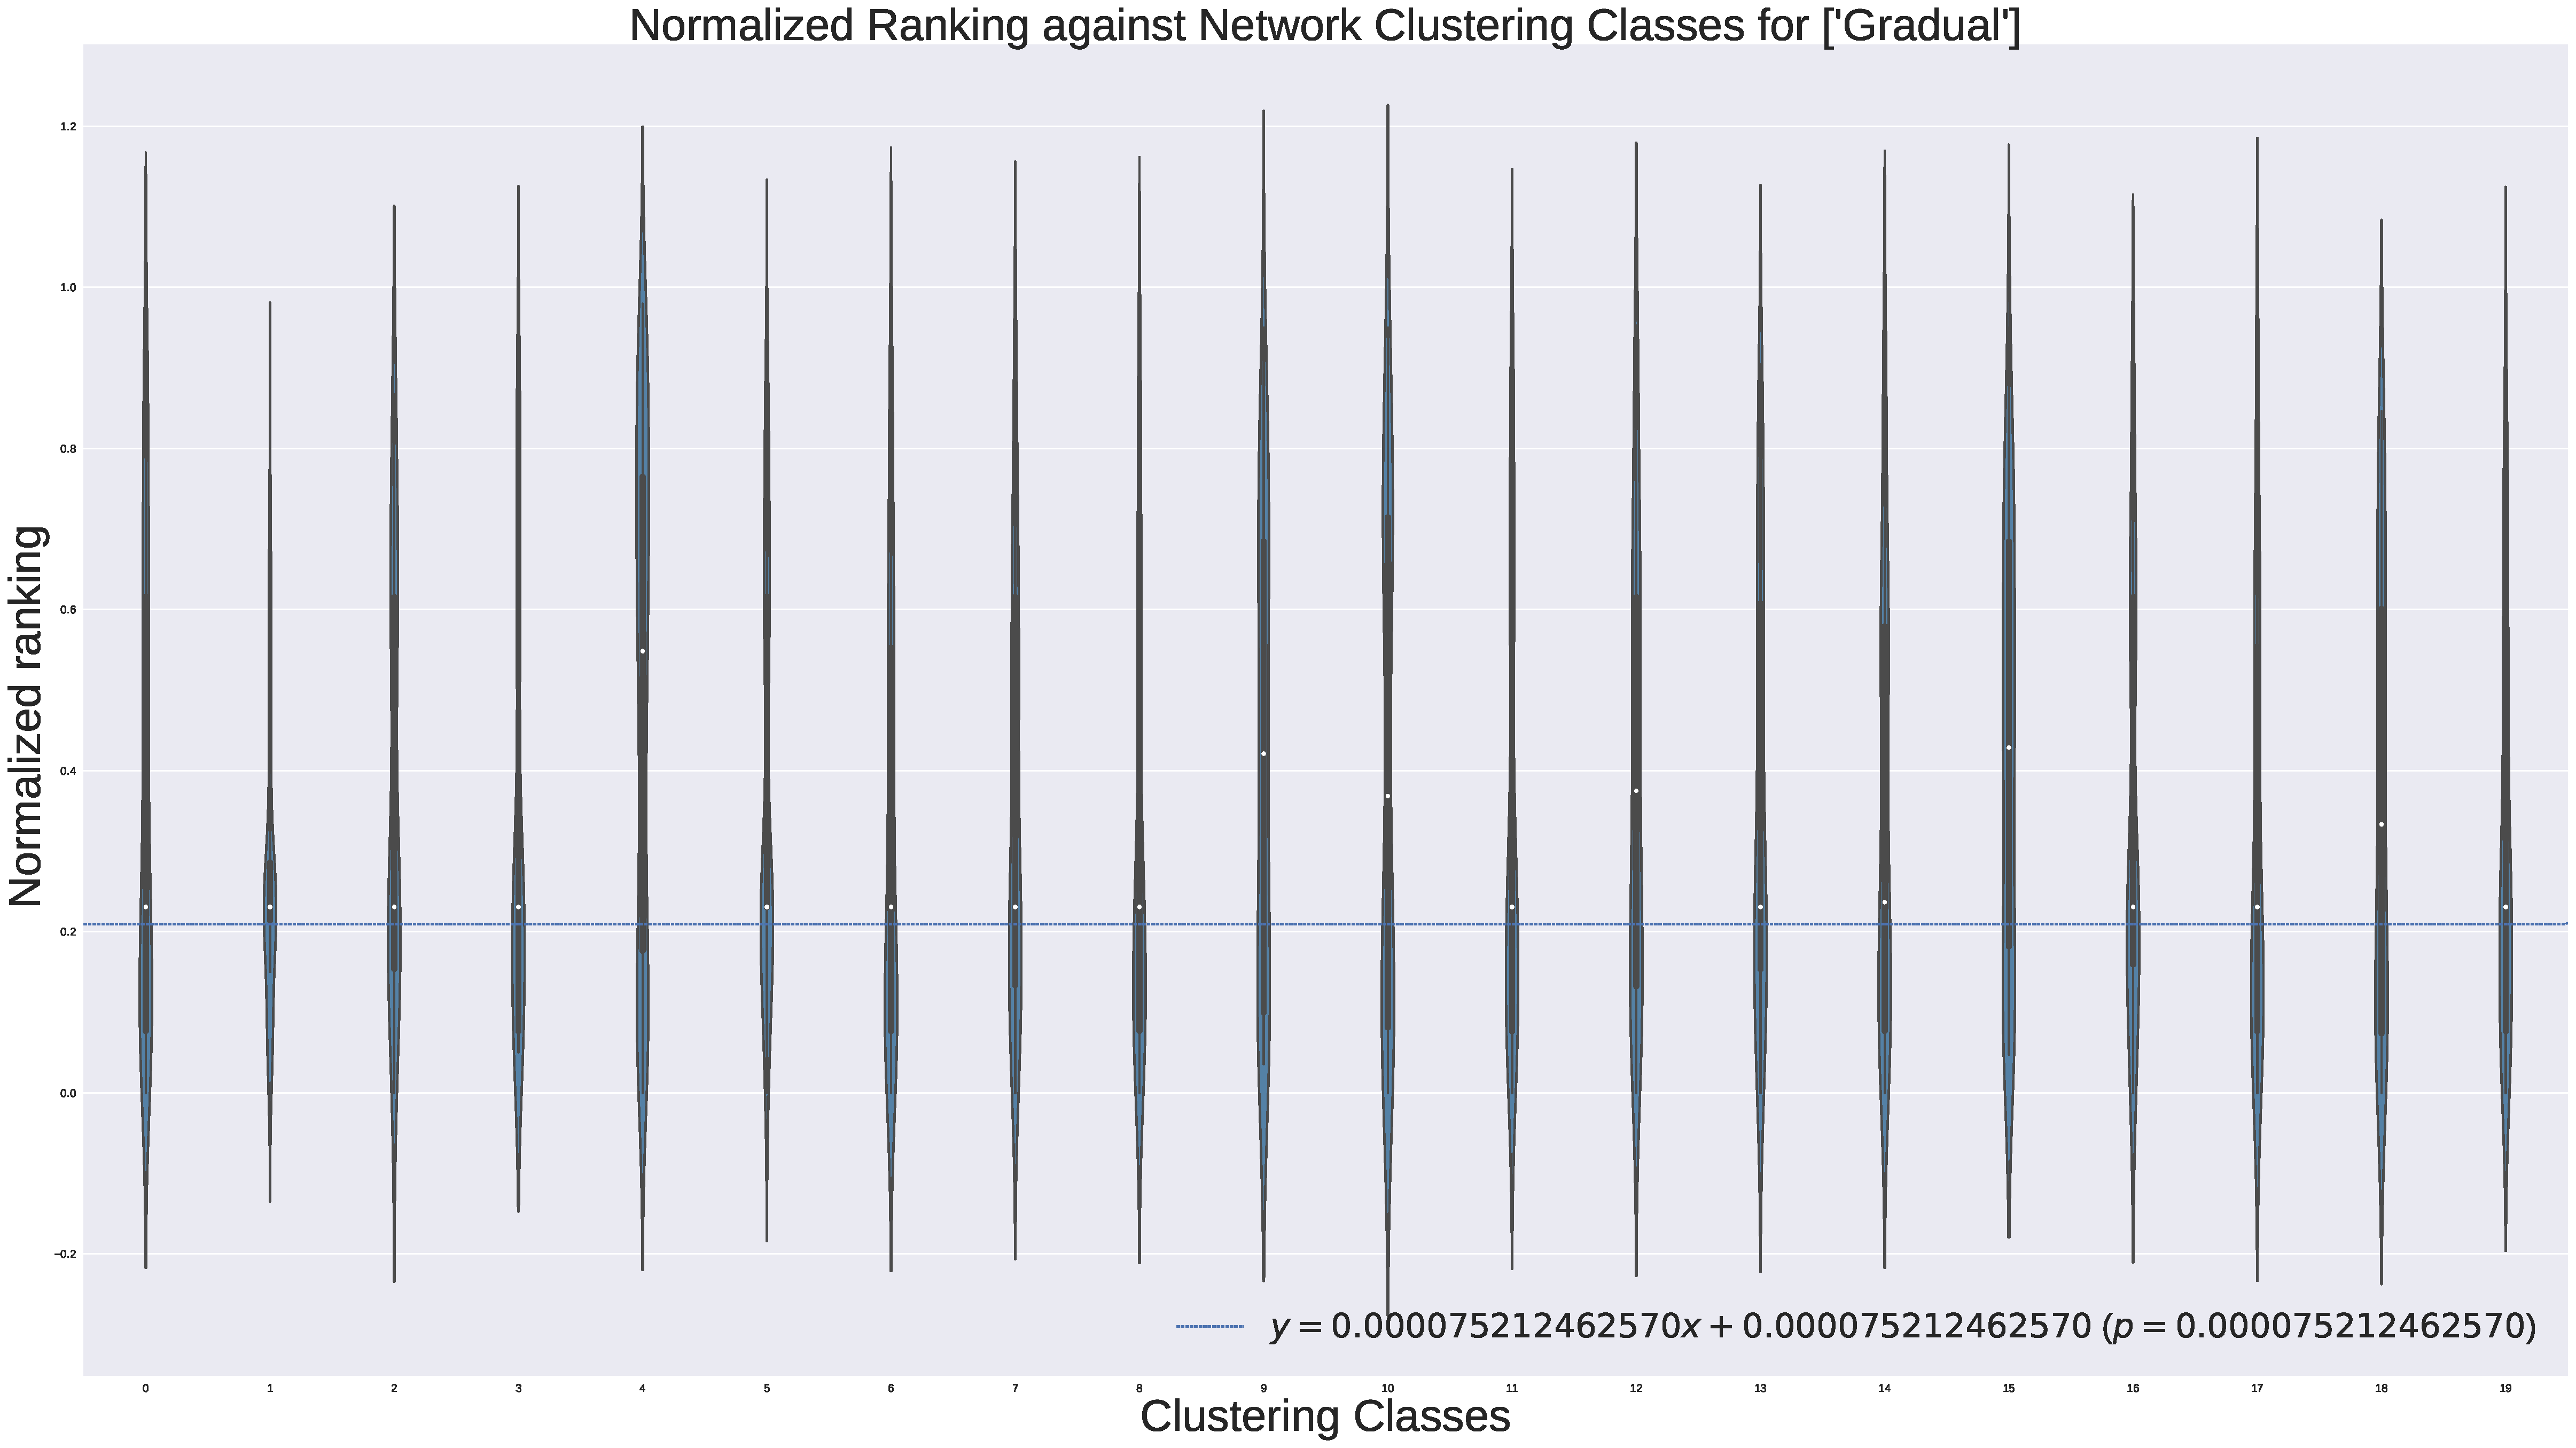
\includegraphics[width=\linewidth]{chapter-four/normalized-rank-['Gradual']-clustering.pdf}
		\caption{Normalized Ranking against Network Clustering Classes}
	\end{subfigure}
	\caption{Normalized Ranking Violin Plots for Gradual}
	\label{gradual}
\end{figure}

In this subsection, the best performed strategies, Nydegger, Cautious QLearner, Gradual,
have been defined based on the median ranking. Furthermore, the difference in
these strategies ranks have been studied, based on groups of network clustering,
connectivity and cooperating ration. The results indicated, statistically significant
difference. The following subsection focal point is building a regression model.

\subsection{Regression}

This subsection concentrates, into build a regression model, for predicting
the normalized ranking of s strategy. This has been done, by identifying any
correlation between the topology measures and the participations of the strategy.
Initially, an analysis was performed for the entire data set, using the following
model.

\begin{align}
	\mathrm{normalised.ranking}_{t} = \alpha
	  & + \beta_{1}  \mathrm{average.neighborhood.score}_{t}          \\
	  & + \beta_{2}  \mathrm{normalized.average.score}_{t}            \\
	  & + \beta_{3}  \mathrm{cooperating.ratio}_{t}                   \\
	  & + \beta_{4}  \mathrm{connectivity}_{t}                        \\
	  & + \beta_{5}  \mathrm{clustering}_{t}                          \\
	  & + \beta_{6}  \mathrm{neighborhood.size}_{t}                   \\
	  & = \beta_{7}  \mathrm{tournament.size}_{t}                     \\
	  & + \beta_{8}  \mathrm{number.of.participations}_{t} + \epsilon
\end{align}

The result of the model have been the following~\ref{regression-complex-networks}.
All the predictors, expect clustering and neighborhood size, are significant.
Due their \(p\) value being less than 0.05.
Apart from normalized average score, connectivity and cooperating ratio, all
variables have a positive correlation with the normalized ranking. Because the
objective function, is to minimize the ranking, normalized average score,
connectivity and cooperating ratio are the only predictors affecting the performance
of a strategy positively. The model itself has a R squared value of 0.014.

\begin{table}[!hbtp]
	\centering
	\begin{adjustbox}{width=0.5\textwidth}
		\small
		\begin{tabular}{|l|l|l|l|}
			\hline
			\multicolumn{4}{|c|}{Regression Results}         \\ \hline
			                           & coefficient & \(p\) value & R-squared \\ \hline
			Intercept                  & 0.3712      & 0.000       & 0.006     \\ \hline
			average.neighborhood.score & 0.0206      & 0.000       & -         \\ \hline
			normalized.average.score   & -0.6150     & 0.001       & -         \\ \hline
			clustering                 & 0.0033      & 0.033       & -         \\ \hline
			connectivity               & -0.0011     & 0.000       & -         \\ \hline
			cooperating.ratio          & -0.0403     & 0.000       & -         \\ \hline
			tournament.size            & 0.0033      & 0.000       & -         \\ \hline
			frequency                  & 1.35e-06    & 0.000       & -         \\ \hline
			neighborhood.size          & 0.0005      & 0.017       & -         \\ \hline

		\end{tabular}
	\end{adjustbox}
	\caption{Regression Results}
	\label{regression-complex-networks}
	explaingn
\end{table}

Furthermore, a model for each of the top ranking strategies has been build.
Using the same model, the individual results are shown in Table~\ref{reg-for-top}.
For Nydegger and Gradual the R square values of the models are low, compared
to Cautious QLeaner. Cuatious QLeaner is the only strategy were more than two
predictors are significant. The findings of these approach are the following,

\begin{itemize}
	\item Nydegger's, performance was significantly affected by clustering of the network
				and the tournament size
	\item Cautious QLearner's, performance was significantly affected by the tournament size
				, the average neighborhood score and the normalized average score
	\item Gradual's, performance can not be anticipated by the model
\end{itemize}

\begin{table}[!hbtp]
	\centering
	\begin{adjustbox}{width=0.7\textwidth}
		\small
		\begin{tabular}{|l|l|l|l|l|l|l|l|l|l|}
			\hline
			\multicolumn{10}{|c|}{Regression Results}                                                                       \\ \hline
			& \multicolumn{3}{l|}{Nydegger} & \multicolumn{3}{l|}{Cautious QLearner} & \multicolumn{3}{l|}{Gradual} \\ \hline
			  & coefficient & \(p\) value & R-squared & coefficient & \(p\) value & R-squared & coefficient & \(p\) value & R-squared    \\ \hline

			Intercept                  &  2.729e-09   & 0.269    & 0.042 		& 1.508e-08  &    0.114   & 0.129		& 8.626e-08   &  0.058 &  0.020       \\ \hline
			average.neighborhood.score &     0.0475   & 0.043    & - 				&    0.1716  &    0.000   & -  			&   -0.0301   &  0.478 &  -					\\ \hline
			normalized.average.score   &   114.0857   & 0.163    & - 				& -653.0862  &    0.000   & - 			&   83.8451   &  0.339 &  -						\\ \hline
			connectivity               &    -0.0019   & 0.316    & - 				&    0.0043  &    0.110   & - 		 	&    0.0006   &  0.838 &  -  					\\ \hline
			clustering                 &    -0.0749   & 0.004    & - 				&   -0.0594  &    0.059   & -  			&   -0.0108   &  0.785 & 	-					\\ \hline
			cooperating.ratio          &     0.0456   & 0.331    & - 				&    0.0673  &    0.497   & - 			&   -0.1310   &  0.082 &  -						\\ \hline
			tournament.size            &     0.0100   & 0.000    & - 				&    0.0176  &    0.000   & - 		  &    0.0037   &  0.080 & 	-						\\ \hline
			frequency                  &  4.884e-06   & 0.758    & -  			& 3.942e-05  &    0.196   & - 			&    0.0002   &  0.054 &  -		 			\\ \hline
			neighborhood.size          &     0.0004   & 0.844    & - 				&   -0.0066  &    0.033   & -  			&    0.0005   &  0.894 &  -						\\ \hline

		\end{tabular}
	\end{adjustbox}
	\caption{Regression results for Nydegger, Cautious QLearner and Gradual}
	\label{reg-for-top}
\end{table}

In this subsection, the performance of the strategies has been tried to be predicted
by a regression model. The results, for running this regression model to the
hole data set returned that cooperating ratio, connectivity and the normalized
average score were significant predictors. Furthermore, the analysis of the model
to each top ranked strategy individual returned, that their performance can not
be accurately predicted by the possible predictors given. In the next section,
a summary of the findings of this chapter have been stated.

\section{Summary}
In this chapter, experiments with more complex networks topologies have been
performed. Networks such as small world, random and complete have been chosen,
and more specifically models, to recreate each of the networks.
Due to the large cpu power and time needed for the experiments, only the complete
experiment, have reached maximum capabilities.
Even so, a data set, created by combining the results retrieved from each experiment,
has been used to carry out the analysis.

Before combining the results, an initial analysis on the networks and their
results has been carried out. For the research on the combined data, a brief
mention on the winning ratio and the normalized average score have been made.
In this chapter, a new measure has been used, the normalized median rank,
and the three top performed strategies of the complex networks experiment have
been named. Nydegger, Cautious QLearner and Gradual.

An analysis on the normalized ranking was then conducted. The findings are the
following. Normalized ranking, for the top strategies have been significantly different
between groups of connectivity, clustering and cooperating. Also cooperating behavior, has been showed to
be affecting the performance. All three strategies have been characterized as highly
cooperators by the analysis in ~\ref{sub:four-classification}. Regression showed that, predicting the
performance of this strategies will not be impossible. Even so, the overall model
did return a few finding compared to~\ref{chap:Three}.

In conclusion, further research with more data and different random topology
is needed. Thought connectivity and cooperating ratio seems to have played a role,
there is not enough validation in the results. The topology does in did affect
the strategies, but a strategy that could outperform any topology has now been
found yet. Whether a strategy like this exist or not in the Axlerod Python Library
is not sure. Thus, in the following chapter an strategy will be trained for
this reason.

% miyagi
